\documentclass[11pt]{article}
\usepackage[margin=1in]{geometry}
\usepackage{amsmath,amsfonts,amssymb,amsthm}
\usepackage[hidelinks]{hyperref}
\usepackage{graphicx}
\usepackage{subcaption}
\usepackage{placeins} % for \FloatBarrier
\usepackage[numbers,sort&compress]{natbib}
\usepackage{comment}

% --- change-marking helpers (compile-safe) ---
% NOTE: ulem/\sout is fragile with \cite and other macros inside long deleted blocks.
% This compile-safe definition keeps deletions visibly marked in red without strikethrough.

% --- small layout helpers to reduce line-overflow warnings ---
\setlength{\emergencystretch}{2em}
\raggedbottom

% --- handy macros ---
\newtheorem{proposition}{Proposition}
% Abbreviations that work in and out of math mode
\makeatletter
\newcommand{\@abbr}[1]{\ifmmode\mathrm{#1}\else\textsc{#1}\fi}
\newcommand{\WEC}{\@abbr{WEC}}
\newcommand{\NEC}{\@abbr{NEC}}
\newcommand{\SEC}{\@abbr{SEC}}
\newcommand{\DEC}{\@abbr{DEC}}
\makeatother

\title{Positive--Energy Seed Constructions for a Restricted Zero--Vorticity Translation Class of Warp--Drive--Like Metrics}
\author{N.~Bol\'ivar$^{a,b}$, G.~Abell\'an$^{a,b}$, I.~Vasilev$^b$ \\
$^a$Departamento de F\'isica, Facultad de Ciencias, Universidad Central de Venezuela \\
Av.~Los Ilustres, Caracas, 1041-A, Venezuela \\
$^b$Astrum Drive Technologies, Dallas Pkwy Unit 120 B, Frisco, 75034, TX, USA}
\date{}

\begin{document}
\maketitle

\begin{abstract}

In this work we analyze a restricted route for constructing warp-drive-like metrics starting from static, spherically symmetric seeds with non-negative energy density. The starting point is a kinematical observation from the zero-vorticity ADM-mass analysis of Santiago, Schuster, and Visser, which we use here as a constructive guide rather than as a no-go statement.

The seeds are piecewise anisotropic-fluid configurations chosen so that $\rho\ge 0$ while the largest tangential stresses are localized in thin shells. Within the class of spatially uniform, time-independent centroid translations, the translated ansatz leaves the seed energy density unchanged in the orthonormal comoving diagnostic frame and transfers the nontrivial response to the spatial stress sector. This does not remove the underlying exoticity problem, but it reorganizes it in a form that can be analyzed explicitly and handled with a simple constrained optimization.

We prove that the energy flux $q_i$ vanishes identically for the uniform-translation ansatz, so the stress-energy tensor is Hawking--Ellis Type~I. This establishes that the principal-stress energy-condition margins are necessary and sufficient for all timelike and null observers, not merely for the comoving diagnostic frame. Using these all-observer diagnostics and differentiable constrained optimization, we examine representative single-shell and double-shell seeds at $v=0.1$ ($c=1$). The sampled configurations still exhibit localized violations of the \NEC, \WEC, and \DEC; however, $\rho$ remains non-negative by construction, the $\DEC$ is typically the tightest residual condition, and the $\SEC$ is less restrictive in aggregate than the $\DEC$ although it is not uniformly positive. The pass/fail threshold used in the numerics ($10^{-9}$) is a floating-point tolerance and should not be interpreted as a physical bound.

Our aim is methodological. The construction presented here provides a restricted but explicit way to generate and optimize families of warp-drive-like metrics whose remaining deficits are stress-dominated and localized, with rigorous all-observer diagnostic status via the Hawking--Ellis classification. In this sense, the present analysis should be understood as a proof of concept for a broader line of model building, with natural extensions to nontrivial lapse functions, spatial conformal factors of Van Den Broeck type, and other ans\"atze beyond the standard Alcubierre/Nat\'ario templates.
\end{abstract}

\section{Introduction}
\label{sec:intro}
The theoretical possibility of warp-drive motion within general relativity has remained one of the most provocative problems in gravitational physics since Alcubierre's original proposal~\cite{Alcubierre:1994tu}. By prescribing a spacetime in which a compact bubble is translated relative to asymptotically flat observers, Alcubierre showed that superluminal \emph{coordinate} motion is not excluded by Einstein's equations even though local causal cones are everywhere respected~\cite{Alcubierre:1994tu,Clark:1999zn,Everett:1995nn}. Subsequent work clarified both the causal interpretation of these geometries and the strong restrictions imposed by their stress--energy content~\cite{Pfenning:1997,Olum:1998mu,Low:1998uy,Lobo:2004wq}.

The main difficulty is also well known: generic warp-drive constructions violate the standard pointwise energy conditions. In particular, physically reasonable warp drives violate the \NEC\ and therefore also the \WEC\ in standard general relativity~\cite{Olum:1998mu,Santiago:2021aup}. At the same time, the literature has shown that the space of possible warp-like ans\"atze is broader than the original Alcubierre form. Nat\'ario reformulated the geometry in terms of a zero-expansion shift vector~\cite{Natario:2001}; Van Den Broeck proposed a conformally modified strategy to reduce integrated energy requirements~\cite{VanDenBroeck:1999}; and more recent work has explored additional constrained subclasses and matter models~\cite{Krasnikov:1998,Bobrick:2021,Lentz:2020euv}. These developments do not remove the no-go results, but they do indicate that there is room for alternative construction strategies.

Motivated by these developments, we follow that direction. In recent work~\cite{Bolivar:2025a}, we constructed static, spherically symmetric seed geometries sourced by piecewise anisotropic fluids with $\rho\ge 0$ by design. These seeds satisfy $p_r=-\rho$, localize large tangential stresses in narrow shells, and provide explicit analytic control over shell amplitude, width, and interface position. Independently, Santiago, Schuster, and Visser showed that for zero-vorticity warp drives with spatially uniform, time-independent centroid motion, the translated ansatz leaves $G_{00}$ unchanged and modifies only the spatial components of the Einstein tensor~\cite{Santiago:2021aup,Schuster:2023ADMmass}. We do not introduce a new mechanism here. Instead, we use that kinematical observation as a restricted construction guide: we start from a positive-energy static seed, embed it into the constant-translation zero-vorticity class singled out in the ADM-mass analysis, and then study the corresponding spatial-stress sector.

The scope of the paper is deliberately limited. We do \emph{not} claim to solve the exotic-matter problem for warp drives, to produce a generic physically viable warp bubble, or to establish the standard energy conditions for all observers. We also do \emph{not} use a physics-informed neural network in the standard sense of Raissi, Perdikaris, and Karniadakis~\cite{Raissi:2019PINN}. Instead, we perform \emph{differentiable constrained optimization} over a low-dimensional analytic ansatz for the seed and for the interface regularization; this term is used throughout the paper in place of ``physics-informed optimization'' to avoid confusion with PINN-based methods. The role of the optimization is therefore modest: once the restricted construction principle is fixed, it helps organize the remaining degrees of freedom in a controlled parameter space.

With that understanding, the paper has three concrete aims. First, we show how the restricted translation-based zero-vorticity construction suggested by~\cite{Santiago:2021aup,Schuster:2023ADMmass} acts on our static piecewise seeds and why it preserves $\rho\ge 0$ under uniform centroid translations. Second, we prove analytically that the energy flux $q_i$ vanishes identically for this ansatz, establishing the Hawking--Ellis Type~I classification of the stress-energy tensor and thereby upgrading the principal-stress diagnostics from preferred-frame checks to all-observer energy-condition tests (Appendix~\ref{app:type1}). Third, we quantify the remaining stress-sector obstruction by means of these all-observer diagnostics and a reproducible differentiable constrained-optimization workflow. For the sampled low-velocity configurations considered here, the resulting hierarchy is empirical rather than universal: the strongest residual obstruction is typically the \DEC, while the \WEC/\NEC\ margins remain substantially constrained and localized rather than disappearing. In this sense, the main contribution of the paper is methodological. The construction developed here provides a restricted but explicit entry point for generating broader families of warp-drive-like metrics, including future extensions with nontrivial lapse functions, spatial conformal factors of Van Den Broeck type, and ans\"atze that need not remain strictly Alcubierre- or Nat\'ario-like.

The remainder of this paper is organized as follows. Section~2 reviews the static seeds, their tetrad formulation, and the piecewise shell constructions. Section~3 describes the restricted translation-based zero-vorticity class and the resulting modification of the Einstein tensor. Section~4 reformulates the numerical section as a reproducible constrained-optimization workflow, clearly defining the diagnostics, trainable variables, sampling procedure, and tolerances. Section~5 discusses the single-shell and double-shell results, emphasizing what is and is not established by the present calculation. Section~6 summarizes the restricted claim of the paper and outlines the most relevant extensions. Appendix~\ref{app:translated-Gab} provides a self-contained derivation of the translated Einstein tensor, and Appendix~\ref{app:type1} establishes the Hawking--Ellis Type~I classification that elevates the principal-stress diagnostics to all-observer energy-condition tests.

\section{Static warp bubbles: metric and seeds}
\label{sec:static}
Our investigation begins with the spherically symmetric warp--bubble configurations that serve as the foundation for the translated zero-vorticity constructions studied here.

\subsection{Static metric and anisotropic stresses}
These static solutions are characterized by the line element
\begin{equation}
\label{eq:static-metric}
ds^2 = -dt^2 + \bigl(dr-\beta(r)dt\bigr)^2 + r^2d\theta^2 + r^2\sin^2\theta\, d\varphi^2,
\end{equation}
whose flat spatial slices are apparent upon $dr^2+r^2d\Omega^2=\delta_{ij}dx^idx^j$ and $dr=\hat r_i dx^i$. The constraint $|\beta(r)| < 1$ keeps $g_{tt}<0$ in this chart and avoids lapse zeros for the present ansatz. Accordingly, no horizon is signalled by this coordinate representation; a separate global causal analysis would be required to make a stronger horizon statement.

To analyse the system and find Einstein's equations directly, we use the local plane frame defined by the following tetrad (Cartan 1-forms)
\begin{eqnarray}\label{eq:tetrad}
    \omega^{0} = dt\,, \quad
    \omega^1 = -\beta dt+dr\,, \quad
    \omega^2 = rd\theta\,, \quad
    \omega^3 = r\sin{\theta}d\varphi\,.
\end{eqnarray}
The dual basis associated with this tetrad is (vector fields)
\begin{eqnarray}
    \partial_{0} = \partial_t + \beta\partial_r\,, \quad
    \partial_1 = \partial_r\,, \quad
    \partial_2 = \frac{1}{r}\partial_\theta\,, \quad
    \partial_3 = \frac{1}{r\sin{\theta}}\partial_\varphi\,, \label{tetrad4}
\end{eqnarray}
with the orthonormal relation $\omega^a(e_b)=\delta^{a}_{\;\,b}$.
The nonzero components of the Einstein tensor are found to be
\begin{eqnarray}
		& & G_{00} = -G_{11} = \frac{\beta}{r^2}\Bigl(2r\,\beta' + \beta\Bigr) \, , \\[2mm]
		& & G_{22} = G_{33} = -\beta\,\beta'' - (\beta')^2 - \frac{2\beta}{r}\,\beta' = 8\pi p_\perp\,.
\end{eqnarray}
Here, primes denote $r$-derivatives. Note the relation $G_{22}=G_{33}$ which is necessary due to the spherical symmetry. From these expressions, the system admits in general the description of anisotropic matter, therefore the energy-momentum tensor is given by
\begin{equation}
T_{ab} = \mathrm{diag}(\rho, p_1, p_2, p_3)\;.
\end{equation}
With the Einstein tensor $G_{ab}$, and the energy momentum tensor $T_{ab}$, we write the independent field equations
\begin{eqnarray}
\label{Gtt-eqn}
& &  \frac{\beta}{r^2}\Bigl(2r\,\beta' + \beta\Bigr) = 8\pi \rho\,, \\[2mm]
\label{Grr-eqn}
& &  -\frac{\beta}{r^2}\Bigl(2r\,\beta' + \beta\Bigr) = 8\pi p_r\,, \\[2mm]
\label{G22-eqn}
 & &  -\beta\,\beta'' - (\beta')^2 - \frac{2\beta}{r}\,\beta' = 8\pi p_\perp\,.
\end{eqnarray}
The Einstein equations yield an anisotropic stress tensor with the hallmark equation of state $p_r=-\rho$.
Because of this equation of state, the radial \NEC/\WEC/\DEC\ inequalities are fulfilled and only the transverse sector is nontrivial. Intuitively, radial null and timelike rays see something like a cosmological constant, so all of the interesting constraint structure is pushed into the tangential stresses.

Finally, the standard pointwise energy conditions for anisotropic fluid then read~\cite{HawkingEllis1973,Barcelo:2000zf}
\begin{align}
\text{NEC}:&\quad \rho + p_i \ge 0\quad (i=1,2,3), \\
\text{WEC}:&\quad \rho \ge 0,\quad \rho + p_i \ge 0\quad (i=1,2,3), \\
\text{DEC}:&\quad \rho \ge |p_i|\quad (i=1,2,3), \\
\text{SEC}:&\quad \rho + p_1 + p_2 + p_3 \ge 0.
\end{align}
In our system, the condition $p_r = -\rho$ means that the radial NEC/WEC/DEC components are exactly saturated, and the nontrivial constraints are carried by the transverse pressure $p_\perp$. Later, in Sec.~\ref{sec:numerics} we recast these conditions in terms of the eigenvalues of the spatial stress tensor $P_{ij}$, which is the form used in our principal-stress diagnostics and optimization.

\subsection{Piecewise seeds and thin shells}
We consider two families of matter distributions. First, a ``single shell'' with vanishing interior and exponentially decaying exterior,
\begin{equation}
\rho(r)=\begin{cases}
 0, & 0\le r<2/b,\\[2pt]
 a\,e^{-br}, & r\ge 2/b,
\end{cases}
\quad\Longrightarrow\quad
\beta(r) = \sqrt{\frac{8\pi a}{b^3 r}\left[10e^{-2} - e^{-br}\bigl(b^2r^2+2br+2\bigr)\right]},
\end{equation}
and second, a ``double shell'' supported on $R\le r\le 2/b$ with tunable inner radius $R$,
\begin{equation}
\rho(r)=\begin{cases}
0, & 0\le r<R,\\[2pt]
\frac{A\,e^{-b(r-R)}}{r^2}, & R\le r \le 2/b,\\[2pt]
0, & r>2/b\,.
\end{cases}
\end{equation}

Both configurations are chosen so that $0<\beta(r)<1$ on their support, again avoiding any lapse zero in the present coordinate representation. For the single-shell profile, a derivative jump can occur at $r=2/b$ if the interface is taken to be sharp; for the double-shell profile, derivative jumps can occur at both $r=R$ and $r=2/b$. In the distributional limit these interfaces are described by the standard Israel--Lanczos junction formalism~\cite{Israel:1966rt,Lanczos:1922,Barrabes:1991ng,Mars:1993gj,Steinbauer:2006qi}. In the numerical optimization, however, we do not evolve truly discontinuous interfaces: we replace the hard support by smooth sigmoid masks so that the sampled stresses remain finite and differentiable.

\section{From static seeds to a restricted translation-based zero-vorticity class}
\label{sec:warp}
To embed the static solutions into the restricted translation-based zero-vorticity class highlighted in~\cite{Santiago:2021aup,Schuster:2023ADMmass}, it is helpful to rewrite the seed metric in Cartesian form. Using $r=\sqrt{x^2+y^2+z^2}$, $\hat r^i=x^i/r$, and $dr=\hat r_i\,dx^i$, the static line element becomes
\begin{equation}
\label{eq:zero-vorticity-line-revised}
\begin{aligned}
ds_0^2
&=-dt^2+\delta_{ij}\,dx^i dx^j-2\beta(r)\hat r_i\,dx^i dt+\beta(r)^2dt^2\\
&=-dt^2+\delta_{ij}\bigl[dx^i-\beta(r)\hat r^i dt\bigr]\bigl[dx^j-\beta(r)\hat r^j dt\bigr].
\end{aligned}
\end{equation}
For spherically symmetric seeds there exists a scalar potential $\Phi(r)$ such that $\nabla^i\Phi=\beta(r)\hat r^i$, so the shift is explicitly of gradient type and the metric belongs to Nat\'ario's zero-vorticity class~\cite{Natario:2001,Schuster:2023ADMmass}. We then translate the profile, $\vec x\mapsto \vec x-\vec x_*(t)$, with centroid velocity $\vec v_*(t)=\dot{\vec x}_*(t)$. In comoving coordinates $\bar x^i=x^i-x_*^i(t)$ one finds
\begin{equation}
\label{eq:comoving-revised}
d\bar s^2=-dt^2+\delta_{ij}\Big[d\bar x^i-(\beta(\bar r)\hat{\bar r}^{\,i}+v_*^i)dt\Big]\Big[d\bar x^j-(\beta(\bar r)\hat{\bar r}^{\,j}+v_*^j)dt\Big].
\end{equation}
Thus the bubble is stationary in the comoving coordinates $\bar x^i$, while asymptotic observers see a centroid moving with velocity $\vec v_*(t)$. In the present paper we work only with spatially uniform, time-independent $\vec v_*$, because that is the regime in which the translation-based zero-vorticity statements are exact.

More generally, as discussed in \cite{Schuster:2023ADMmass}, the line element for a warp drive with zero vorticity takes the generic form
\begin{equation}
\label{eq:zero-vorticity}
ds^2 = -dt^2 + \delta_{ij} (dx^i - \nabla^i\Phi(t,\vec{x})dt)(dx^j - \nabla^j\Phi(t,\vec{x})dt),
\end{equation}
where writing the metric function as a gradient $\nabla^i\Phi$ guarantees by construction the condition of zero vorticity. The most intuitive way to make the metric function time-dependent and ensure centroid displacement is through the substitution $\Phi(t,\vec{x}) \to \Phi(\vec{x} - \vec{x}_*(t))$.
This transformation shows how warp-drive construction can begin from a base spacetime
\begin{equation}
\label{eq:base-space}
ds^2_0 = -dt^2 + \delta_{ij} (dx^i - \nabla^i\Phi(\vec{x})dt)(dx^j - \nabla^j\Phi(\vec{x})dt),
\end{equation}
and then perform a spatial coordinate translation. The asymptotic condition $\Phi(\vec{x}) \to 0$ as $r \to \infty$ ensures that
\begin{equation}
    ds^2_\infty = -dt^2 + \delta_{ij} dx^i dx^j\,.
\end{equation}
That is, the spacetime is asymptotically flat. A particularly useful approach involves transform to comoving coordinates with the warp bubble
\begin{equation}
t = t, \quad \bar{x}^i = x^i - x^i_*(t) \quad \Rightarrow \quad dt = dt, \quad d\bar{x}^i = dx^i - v^i_*(t)dt,
\end{equation}
where $v^i_*(t) = dx^i_*/dt$ represents the bubble's velocity. In these coordinates, the line element becomes
\begin{equation}
\label{eq:comoving-line-element}
d\bar{s}^2 = -dt^2 + \delta_{ij} \left[d\bar{x}^i - (\nabla^i\Phi(\vec{\bar{x}})+v_*^i(t))dt\right]\left[d\bar{x}^j - (\nabla^j\Phi(\vec{\bar{x}})+v_*^j(t))dt\right].
\end{equation}
At spatial infinity, this reduces to
\begin{equation}
d\bar{s}^2_\infty = -dt^2 + \delta_{ij} (d\bar{x}^i - v_*^i(t)dt)(d\bar{x}^j - v_*^j(t)dt),
\end{equation}

showing that the bubble is stationary in comoving coordinates while asymptotic observers measure the centroid velocity $v_*^i(t)$. In this paper we restrict attention to the low-velocity example $v_*=0.1$ and do not make any separate claim based solely on coordinate superluminality.

\subsection{Restricted spatial-stress modification}
In the orthonormal comoving frame adapted to the warp bubble we take the tetrad 1-forms
\begin{align}
e^0 &= dt, \\
e^i &= dx^i - \bigl(\hat{r}^i\beta(r) + v^i_*(t)\bigr)\,dt,
\end{align}
with dual vectors
\begin{align}
e_0 &= \partial_t + \bigl(\hat{r}^i\beta(r) + v^i_*(t)\bigr)\partial_i, \\
e_i &= \partial_i.
\end{align}

We adopt this orthonormal comoving frame as the diagnostic frame for the effective source, so that the energy flux components satisfy $q_i=0$ for the seed configurations and for the uniformly translated warped configurations considered here.

Given that the lapse function is trivial ($\alpha=1$) and using \eqref{eq:zero-vorticity-line-revised}, we move spatial indices up and down with $\delta_{ij}$. So we write $\beta_i(t,\vec x)=\beta(r)\hat r_i+v^*_i(t)$ with \emph{spatially uniform} $v^*_i(t)$. Then the spatial components of extrinsic curvature $K_{ij}=\tfrac12(\partial_i\beta_j+\partial_j\beta_i)$ are unchanged by adding the uniform velocity field $v^*_i(t)$ (see \cite{Schuster:2023ADMmass}). What is useful about this construction, when applied to a static seed spacetime, is that it produces an Einstein tensor with clearly differentiated terms
\begin{equation}
G_{00}=(G_0)_{00}\,,\qquad G_{0i}=(G_0)_{0i}\,, \qquad
G_{ij}= (G_{0})_{ij} + v^{k}_{*}(t)  \partial_{k}[K_{ij}-K\delta_{ij}]
\,.
\end{equation}
Thus, by Einstein's equations, the stress--energy tensor inherits the same structure,
\begin{equation}
T_{00}=(T_0)_{00}\,,\qquad T_{0i}=(T_0)_{0i}\,, \qquad
T_{ij}= (T_{0})_{ij} + v^{k}_{*}(t)  \partial_{k}[K_{ij}-K\delta_{ij}]\,,
\end{equation}
so only spatial stresses $T_{ij}$ are affected by motion through gradients of the shift
\cite{Santiago:2021aup,Schuster:2023ADMmass}.

Comparing with our material sector for the seed solution, we see that only modifications are introduced in the pressures (radial and tangential). Since there is no heat flow in the seed solution, there will be none in the translated configuration either. Finally, the energy density in the orthonormal comoving diagnostic frame is equal to that of the seed solution. What is remarkable here is therefore limited but useful: if we start with a seed with positive energy density, this restricted translation-based construction preserves that positivity in the same diagnostic frame. Moreover, as shown in Appendix~\ref{app:type1}, the vanishing of the energy flux $q_i$ for this ansatz implies that $T^a{}_b$ is Hawking--Ellis Type~I, so the principal-stress diagnostics computed in the comoving frame are in fact all-observer energy-condition tests (Proposition~\ref{prop:type1-ec}). This does not solve the exotic-matter problem---the sampled configurations still exhibit localized \NEC/\WEC/\DEC\ violations---but it provides a construction angle in which the residual obstruction is shifted into the stress sector and can be studied and optimized with rigorous diagnostic status.

\subsection{Linear-shift similarity and the \texorpdfstring{$vt$}{vt} degeneracy}
\label{sec:vt-similarity}
For the zero-vorticity (Nat\'ario) class with a \emph{linear} constant centroid motion we have
\begin{equation}
    \Phi(t,\mathbf x)=\Phi\big(\mathbf x-\mathbf x_*(t)\big),\qquad \mathbf x_*(t)=\mathbf v_*\,t,\qquad \mathbf v_* = \text{const}\;.
\end{equation}
The translated metric is obtained from the static seed by a rigid spatial translation of the bubble centroid. The shift vector naturally decomposes into
\begin{equation}
    \beta_i(t,\bar{\mathbf x})=\beta(\bar r)\,\hat{\bar r}_i + v^*_{i},\qquad \bar{\mathbf x}=\mathbf x-\mathbf v_* t\,,
\end{equation}
where the first term encodes the bubble profile and the second represents the constant boost. Since the extrinsic curvature $K_{ij}=\tfrac12(\partial_i\beta_j+\partial_j\beta_i)$ involves only spatial derivatives, the constant velocity $v^*_i$ does not contribute with any gradients. Consequently, $K_{ij}$ and the ADM constraints coincide exactly with those of the static seed ~\cite{Arnowitt:1962hi,Wald1984ucp,Alcub2008itnr}. Moreover, for flat spatial slices, the stress--energy tensor in the orthonormal fluid frame equals its static counterpart evaluated at $\bar r=\|\mathbf x-\mathbf v_* t\|$ (see \cite{Santiago:2021aup,Schuster:2023ADMmass} for more details).

This observation leads to a useful degeneracy. The diffeomorphism $\mathbf x\mapsto\mathbf x-\mathbf v_* t$ maps the static seed to the line element
\[
ds^2=-dt^2+\delta_{ij}\big[dx^i-(\nabla^i\Phi(\bar{\mathbf x})+v_*^i)dt\big]\big[dx^j-(\nabla^j\Phi(\bar{\mathbf x})+v_*^j)dt\big],
\]
but the Einstein tensor and all scalar invariants depend only on $K_{ij}$, which is independent of the uniform boost. Therefore, for any two pairs $(v_1,t_1)$ and $(v_2,t_2)$ satisfying $v_1 t_1=v_2 t_2$, the equal-time slices of all physical quantities---energy density $\rho$, pressure trace $\mathrm{tr}\,P$, energy-condition margins---coincide up to a rigid spatial translation $\Delta\mathbf x=\mathbf v_2 t_2-\mathbf v_1 t_1$. In bubble-centered (comoving) coordinates, where $\bar{\mathbf x}$ is held fixed, the configurations are completely identical.

This $vt$ degeneracy has immediate practical consequences: all our slice diagnostics of energy conditions (\WEC/\NEC/\DEC/\SEC) computed at fixed $v_*=0.1$ represent the entire similarity class with the same displacement $d=\|\mathbf v_* t\|$. Within this constant-velocity, zero-vorticity class, bubble-centered diagnostics depend on the displacement and not independently on $v_*$ and $t$. A slow bubble over a long time and a fast bubble over a short time therefore produce identical bubble-centered diagnostics. The degeneracy is broken when the centroid motion becomes non-uniform ($\dot{\mathbf v}_*\neq0$), introducing Lie-derivative corrections $\mathcal{L}_\beta K_{ij}$~\cite{Santiago:2021aup}, or when additional sources, fields, nontrivial lapse functions, conformal spatial factors, or boundary conditions break translational invariance.


\section{Numerical diagnostics and differentiable constrained optimization}
\label{sec:numerics}

This section states the computational problem explicitly. The input is a low-dimensional analytic seed ansatz---single shell: amplitude $a$ and inverse length scale $b$; double shell: $(A,b,R_0)$---together with smooth interface-mask parameters. The output is a sampled stress tensor for the translated zero-vorticity geometry at fixed $(v_*,t)$. The numerical task is therefore a differentiable constrained-optimization problem over a finite set of seed and regularization parameters. It is not a PINN-based PDE solve.

We now describe the diagnostics used to evaluate the stress tensor and the optimization scheme that tunes the shell parameters and interface profiles.  Because energy conditions are observer-dependent statements, we work in the orthonormal comoving frame defined in Sec.~\ref{sec:warp}. In that frame the spatial stress tensor is denoted by $P_{ij}$, while $q_i$ denotes the energy flux. For the seed solutions and for the uniformly translated warped configurations considered here, $q_i=0$ in the chosen frame by construction.

The diagnostics reported below are principal-stress diagnostics computed in the orthonormal comoving frame. As shown in Appendix~\ref{app:type1}, the energy flux $q_i$ vanishes identically for the translated zero-vorticity ansatz with uniform centroid velocity, so the stress-energy tensor $T^{a}{}_{b}$ is block-diagonal and therefore Hawking--Ellis Type~I at every regular grid point~\cite{HawkingEllis1973,Maeda:2022vld,MartinMoruno:2017exc}. For Type~I tensors, the principal-stress margins are \emph{necessary and sufficient} for the pointwise energy conditions to hold for \emph{all} timelike and null observers (Proposition~\ref{prop:type1-ec}). The diagnostics are therefore not restricted to a single preferred frame.

Specifically, our diagnostics implement $\rho+\lambda_i\ge 0$ (\NEC/\WEC, $i=1,2,3$), $\rho\ge |\lambda_i|$ (\DEC, $i=1,2,3$), and $\rho+\lambda_1+\lambda_2+\lambda_3\ge 0$ (\SEC), where $\lambda_i$ are the eigenvalues of the spatial pressure tensor $P_{ij}$. As emphasized in Ref.~\cite{Santiago:2021aup}, positivity of $\rho$ for one preferred observer family is not, by itself, a \WEC\ result; the Type~I classification established in Appendix~\ref{app:type1} is what allows the principal-stress margins to serve as all-observer tests.

\subsection{Computation: seeds, sampling, and optimization}
\label{sec:comp}
For reproducibility, each optimization run is specified by: (i) the shell topology (single or double); (ii) the initial seed parameters; (iii) the sampling grid and masking prescription; (iv) the fixed kinematic parameters $(v_*,t)$; and (v) the loss weights. Input parameter histories are stored in comma-separated-value (CSV) files, which provide the initial seeds and also record the training histories exported by the code.

We import the piecewise parameters $(a,b)$ (single shell) or $(A,b,R)$ (double shell) from comma-separated-value (CSV) files and construct $\beta(r)$ exactly in each domain. For the static, purely radial analysis we use analytic derivatives piecewise. For the fully dynamic runs we evaluate $\beta$ and its spatial derivatives on a Cartesian grid. Space is sampled on meridional and equatorial slices with masking near $r=0$ and at the shell interfaces. Unless otherwise stated, the results shown below correspond to a single snapshot with fixed $v_*=0.1$ and fixed displacement parameter $d=\|\mathbf v_* t\|$. Plots use a zero-centered diverging blue$\to$white$\to$red colormap: \emph{blue} marks regions where the plotted quantity is negative (energy-condition violation or negative margin), \emph{white} corresponds to values near zero (saturation), and \emph{red} indicates positive values (condition satisfied). The field maps are intended as qualitative spatial diagnostics---they show \emph{where} violations are localized and how the morphology depends on topology---rather than as precision measurements of the margin amplitudes. Quantitative success fractions and representative extrema are reported in Table~\ref{tab:summary}. Color bars are omitted to keep the figures at journal page scale; the relevant numerical values are in the table and in the text.

The optimization reported here does not vary the centroid velocity profile. The trainable variables are only the seed parameters and the interface regularization parameters. For the single-shell topology these are $(a,b)$ plus the mask width; for the double-shell topology they are $(A,b,R)$ plus the mask width. The single shell is simulated on $0\le r\le r_{\text{cap}}$, where $r_{\text{cap}}$ is chosen so the exponential tail is negligible; the double shell uses $R\le r\le 2/b$.

\subsubsection{Differentiable constrained optimization}
Our optimization is ``physics-informed'' only in the mild sense that the loss function is built from geometrically and physically motivated diagnostics of the stress tensor, and gradients are obtained by automatic differentiation through the numerical pipeline. No neural network is trained to represent the spacetime fields. To avoid confusion with PINN-based methods, we refer to this procedure as \emph{differentiable constrained optimization} throughout.
We co-optimize the seed parameters and interface gradients under a composite objective
\[
\mathcal{L}_\text{tot} = \mathcal{L}_\text{phys} + \mathcal{L}_\text{smooth} + \mathcal{L}_{\kappa} + \mathcal{L}_\text{shear},
\]
where the last term is set to zero in the runs shown here but is available as an optional regularizer. The trainable parameters are the seed amplitudes and length scales $(a,b)$ (single shell) or $(A,b,R_0)$ (double shell), together with the smoothing scale $\kappa_{\rm mask}$ that controls the steepness of the sigmoid mask. All of them are represented by unconstrained variables mapped through softplus transformations and (for $b$ and $R_0$) bounded intervals, as summarized in the next subsection.

The physics term $\mathcal{L}_\text{phys}$ penalizes violations of the principal-stress energy-condition margins defined in Sec.~\ref{sec:numerics}. At each grid point we diagonalize $P_{ij}$ to obtain eigenvalues $\lambda_i$ and form the \NEC, \WEC, and \DEC\ margins
\begin{equation}
m_\text{NEC} = \rho + \lambda_{\min},\qquad
m_\text{WEC} = \rho + \min(\lambda_{\min},0),\qquad
m_\text{DEC} = \rho - \max(|\lambda_1|,|\lambda_2|,|\lambda_3|),
\end{equation}
with $\lambda_{\min}=\min_i\lambda_i$. Here $m_\text{WEC}$ is
\[
m_\text{WEC} = \min(\rho,\rho+\lambda_{\min}),
\]
implemented as $\rho + \min(\lambda_{\min},0)$; this packages the usual $\rho\ge0$ and $\rho+p_i\ge0$ requirements into a single scalar margin. Margins are considered acceptable if $m\ge -\delta$ with a small tolerance $\delta\simeq10^{-9}$. Deficits below this threshold are penalized by a smooth one-sided function that grows approximately linearly for small violations and quadratically for larger ones. The physics loss is the soft-mask–weighted average of these penalties,
\begin{equation}
\mathcal{L}_\text{phys} = \kappa_\text{phys}\,\Bigl\langle
\Phi(m_\text{NEC}) + \Phi(m_\text{WEC}) + w_\text{DEC}\,\Phi(m_\text{DEC})
\Bigr\rangle_w,
\end{equation}
where $\langle\cdot\rangle_w$ denotes averaging with weights given by the smooth domain mask $w(r)$, $\kappa_\text{phys}$ is a scaling factor, and $w_\text{DEC}=0.25$ downweights the \DEC\ relative to the null and weak conditions. In this way we treat the energy conditions as soft constraints: violations are allowed but strongly disfavoured.

Operationally, the physics loss provides an integral measure of the energy-condition deficits across the warp bubble. At each grid point we compute the NEC, WEC, and DEC margins from the principal stresses; points that satisfy the conditions within the numerical tolerance contribute nothing, while points that violate them contribute a penalty that increases with the size of the deficit. The physics loss is then the mask-weighted average of these local penalties. Minimizing it drives the optimization toward reduced and localized energy-condition violations, while preserving $\rho\ge 0$ by construction of the static seed. The absolute scale of $\mathcal{L}_\text{phys}$ is fixed by $\kappa_\text{phys}$ and carries no direct physical meaning; the relevant information is the relative decrease and eventual plateau of the loss.

The interface term $\mathcal{L}_\text{smooth}$ measures how well the sigmoid mask $w(r)$ reproduces the intended hard support of the shell. We estimate a false-negative rate (points inside the hard domain where $w$ is close to zero) and two false-positive rates on the vacuum side (points in the interior or exterior vacua where $w$ is non-negligible). These are combined into a single mismatch metric $E_\text{tot}$, and a quadratic penalty is applied only if this mismatch exceeds a target tolerance $E_\text{target}$ (here $E_\text{target}=1\%$):
\begin{equation}
\mathcal{L}_\text{smooth} = \lambda_\text{smooth}\,\max(E_\text{tot} - E_\text{target},0)^2.
\end{equation}
This encourages the soft mask to approximate the sharp domain boundaries without forcing an exactly discontinuous profile.

Finally, the inverse-$\kappa_{\rm mask}$ regularizer
\begin{equation}
\mathcal{L}_{\kappa} = \lambda_{\kappa}/\kappa_{\rm mask}
\end{equation}
discourages arbitrarily steep masks. Combined with the epoch-dependent floor $\kappa_{\rm floor}(\text{epoch})$ described below, this yields sigmoids that are sharp enough to localize the shell while remaining numerically stable in finite-difference derivatives.

In the training logs and in Figs.~\ref{fig:d1-opt}--\ref{fig:d2-opt}, the individual contributions to $\mathcal{L}_\text{tot}$ are recorded as \emph{physics\_loss} ($=\mathcal{L}_\text{phys}$), \emph{reg\_breach} (the interface-mismatch penalty $\mathcal{L}_\text{smooth}$), and \emph{inv\_alpha} (the inverse-width regularizer, denoted analytically here by $\mathcal{L}_{\kappa}$). The curve labelled \emph{total\_loss} tracks their sum $\mathcal{L}_\text{tot}$. All four are normalized by their initial values so that their relative evolution can be compared on a single vertical scale.

To avoid poor local minima, we use a short Monte--Carlo pre-training stage: for each shell topology (single or double) we draw several random initial seeds $(a,b)$ or $(A,b,R_0)$ from broad priors, run a few dozen optimization epochs, and retain the snapshot with the lowest $\mathcal{L}_\text{tot}$ as the starting point for the main run. The main optimization then uses the Adam optimizer with learning rate $3\times10^{-3}$, gradient clipping, and $\mathcal{O}(10^3)$--$10^4$ gradient steps on a $48^3$ Cartesian grid for each snapshot.

Representative training curves are shown in Figs.~\ref{fig:d1-opt} and~\ref{fig:d2-opt}. Panels~\ref{fig:d1-loss-components} and~\ref{fig:d2-loss-components} display the normalized loss components. In the regenerated runs, the total loss decreases and then stabilizes as the interface-mismatch term is driven to zero and the inverse-$\kappa_{\rm mask}$ regularizer controls the late-time balance, while the exported physics term remains numerically small throughout. Panels~\ref{fig:d1-success} and~\ref{fig:d2-success} show the corresponding fraction of grid points that satisfy the NEC, WEC, DEC, and SEC at each epoch. These fractions settle into topology-dependent plateaus in which SEC is the easiest condition to satisfy, DEC is the tightest, and NEC/WEC remain intermediate but still substantially constrained. Finally, the parameter trajectories in panels~\ref{fig:d1-params-epoch} and~\ref{fig:d2-params-epoch} illustrate that the visible main runs stay in narrow parameter bands after Monte--Carlo pretraining has already selected favorable starting snapshots. We take the combination of loss stabilization, reproducible success-fraction plateaus, and parameter stationarity as our practical convergence criterion for a given topology and $(v_*,t)$.

\subsubsection{Parameter representation}
The warp-bubble configuration is represented through optimizable TensorFlow variables with positivity enforced by softplus transformations. In the single-shell case these variables correspond to the analytic parameters $(a,b)$ of Sec.~\ref{sec:static}, and in the double-shell case to $(A,b,R_0)$.

\paragraph{Notation convention.}
Throughout Sec.~\ref{sec:static}, the seed parameters for the single shell are denoted $(a,b)$ and for the double shell $(A,b,R)$. In the optimizer logs and in Figs.~\ref{fig:d1-opt}--\ref{fig:d2-opt}, the code labels these as $(A,B)$ (single shell) and $(A,B,R_0)$ (double shell), with $B\equiv b$ in both cases. We retain both notations in their respective contexts to avoid discrepancies between the figures and the source code, but emphasize that the underlying parameters are the same: $A$ or $a$ is the amplitude, $B$ or $b$ is the inverse length scale, and $R_0$ is the inner shell radius (double shell only). Table~\ref{tab:summary} uses the analytic notation $(a,b)$ and $(A,b,R_0)$.
\begin{align}
A &= \mathrm{softplus}(A_{\text{raw}}) + \epsilon, \\
b_{\mathrm{opt}} &= B_{\min} + \mathrm{softplus}(b_{\mathrm{opt,raw}}) + \epsilon \quad \text{(single shell, with } B_{\min} = 2 / (r_{\text{cap}} - \epsilon_{\text{cap}})\text{)}, \\
b &= \mathrm{softplus}(B_{\text{raw}}) + \epsilon \quad \text{(double shell)},
\end{align}
where $\epsilon = 10^{-6}$ provides numerical stability. For the double shell, $R_0$ is mapped via
\[
R_0 = R_{\min} + \sigma(R_{0,\text{raw}}) \cdot (2/b - 2R_{\min}),
\]
with $\sigma$ the sigmoid and $R_{\min} = 0.02$ a margin. The smoothing parameter $\kappa_{\rm mask}$ is either fixed, scheduled, or trainable with a linearly increasing floor:
\[
\kappa_{\text{floor}}(\text{epoch}) = \kappa_{\text{start}} + t \cdot (\kappa_{\text{end}} - \kappa_{\text{start}}),
\]
where $t = \min(\text{epoch} / (\eta N_{\text{epochs}}), 1)$ and $\eta$ is the warmup fraction (typically $1.0$). For trainable $\kappa_{\rm mask}$,
\[
\kappa_{\rm mask} = \mathrm{softplus}(\kappa_{\text{raw}}) + \kappa_{\text{floor}}.
\]

\subsubsection{Energy-condition evaluation}
The Einstein tensor for the translated metric is evaluated numerically on a discretized mesh covering $(x,y,z)\in[\min,\max]^3$ and $t\in[t_{\min},t_{\max}]$. For computational efficiency we use a reduced snapshot with $N_{xyz}=48$ and $N_t=1$. On this grid we compute $\beta(r)$ and its derivatives using finite differences with step $h=10^{-4}$:
\begin{align}
\beta'(r) &= \frac{\beta(r+h) - \beta(r-h)}{2h}, \\
\beta''(r) &= \frac{\beta(r+h) - 2\beta(r) + \beta(r-h)}{h^2},
\end{align}
with safeguards to ensure finiteness. The dynamic components yield $\rho$ and the spatial stresses $P_x,P_y,P_z,T_{xy},T_{xz},T_{yz}$. We evaluate principal-stress margins using the eigenvalues $\lambda_1\le\lambda_2\le\lambda_3$:
\begin{align}
\text{NEC}_{\min} &= \rho + \lambda_{\min}, \\
\text{WEC}_{\min} &= \rho + \min(\lambda_{\min}, 0), \\
\text{DEC}_{\text{margin}} &= \rho - \max(|\lambda_1|, |\lambda_2|, |\lambda_3|),
\end{align}
where $\lambda_{\min}=\min(\lambda_1,\lambda_2,\lambda_3)$. 
The pass/fail threshold $10^{-9}$ is used only as a floating-point tolerance in the code units of the numerical implementation. It should not be interpreted as a phenomenological bound on physical stress scales. In the text, a margin is counted as numerically passing when it is non-negative up to this tolerance.

\paragraph{Implementation.}

The optimization is implemented in TensorFlow~2.x and executed in a Jupyter environment on commodity cloud hardware. For each shell geometry and each fixed $(v_*,t)$ we run an independent optimization that exports (i) the initial seed parameters, (ii) the full epoch-by-epoch loss history, (iii) the epoch-by-epoch parameter history, and (iv) the final sampled diagnostics used in the figures. The cleaned optimization, diagnostics, plotting, and verification workflow used in this study is publicly archived in the Zenodo software release~\citep{Bolivar_Abellan_Vasilev_2026_warp_optimization}. The archive includes the source code, the regenerated single-shell and double-shell golden bundles used for the manuscript-level claims, and direct evaluations of the manuscript target parameters under the same diagnostics. These materials are sufficient to reproduce the reported bundle summaries and field-map figures.

For readability, the heat maps shown in Figs.~\ref{fig:d1-xy-energy-A}--\ref{fig:d2-xz-energy-B} use a display-only manuscript rendering preset that applies mild zero-centered whitening and local smoothing. For the signed margin maps (WEC, NEC, DEC, SEC), we also show a tighter plotting window around the shell so that the localized residual structure remains visible at journal page scale. This post-processing is used only for visualization. All reported success fractions, principal-stress margins, and optimization diagnostics are computed from the unsmoothed fields exported by the pipeline and are not recalculated from the display-processed images.

\paragraph{Scope of the numerics.}
The numerical results reported here are slice-based and grid-based. They do not constitute a proof of global regularity or a proof that the same hierarchy persists outside the sampled parameter ranges. However, as established in Appendix~\ref{app:type1}, the Hawking--Ellis Type~I classification of $T^a{}_b$ for the present ansatz guarantees that the principal-stress margins are all-observer energy-condition tests, not merely preferred-frame diagnostics. The role of the numerics is therefore to demonstrate that within the zero-vorticity, constant-translation class, positive-energy seeds embedded in the translated ansatz can be optimized so that the residual deficits are stress-dominated and sharply localized, with diagnostic status that extends to all timelike and null observers.

\subsection{Quantitative summary and convergence}
\label{sec:quantitative}

Table~\ref{tab:summary} collects the final optimized parameters and all-observer energy-condition success fractions for the two shell topologies at the manuscript configuration $(v_*=0.1, t=30)$, evaluated at three grid resolutions ($N_{xyz}\in\{48,64,96\}$). The Hawking--Ellis Type~I classification is confirmed numerically at every masked grid point across all six runs, with a maximum energy flux $\|q\|_\infty < 10^{-6}$ (consistent with the analytic proof $q_i\equiv 0$ in Appendix~\ref{app:type1}).

\begin{table}[htbp]
\centering
\caption{All-observer energy-condition success fractions and Hawking--Ellis Type~I verification for optimized single-shell ($a=0.970$, $b=1.321$) and double-shell ($A=1.848$, $b=1.135$, $R_0=1.292$) configurations at $v_*=0.1$, $t=30$. Type~I\% refers to the masked-shell fraction. The ordering $\DEC < \NEC \approx \WEC < \SEC$ is stable across all resolutions, confirming that the hierarchy is geometric rather than a grid artifact.}
\label{tab:summary}
\vspace{0.5ex}
\begin{tabular}{l c c c c c c c}
\hline\hline
Topology & $N_{xyz}$ & Type~I\% & \NEC\% & \WEC\% & \DEC\% & \SEC\% & $\|q\|_\infty$ \\
\hline
Single shell & 48 & 100.0 & 28.7 & 28.5 & \phantom{0}0.9 & 53.8 & $3.8\times10^{-8}$ \\
             & 64 & 100.0 & 28.8 & 28.6 & \phantom{0}0.9 & 53.6 & $1.5\times10^{-7}$ \\
             & 96 & 100.0 & 29.3 & 29.3 & \phantom{0}0.7 & 54.8 & $1.5\times10^{-7}$ \\
\hline
Double shell & 48 & 100.0 & 16.5 & 16.5 & \phantom{0}4.4 & 32.5 & $7.6\times10^{-8}$ \\
             & 64 & 100.0 & 26.2 & 26.2 & \phantom{0}2.3 & 52.4 & $3.0\times10^{-7}$ \\
             & 96 & 100.0 & 24.8 & 24.8 & \phantom{0}3.4 & 53.7 & $6.1\times10^{-7}$ \\
\hline\hline
\end{tabular}
\end{table}

The key observations from Table~\ref{tab:summary} are as follows. (i)~The \DEC\ remains the tightest constraint across all resolutions and both topologies, with success fractions below 5\%. (ii)~The \NEC/\WEC\ margins are intermediate and the \SEC\ is the least restrictive. (iii)~The \emph{qualitative ordering} $\DEC < \NEC \approx \WEC < \SEC$ is robust under grid refinement from $48^3$ to $96^3$ for both topologies. (iv)~The absolute success fractions are resolution-stable for the single shell (varying by $\lesssim 1$~percentage point), but show more noticeable resolution dependence for the double shell: the double-shell \NEC/\WEC\ fractions increase from $\sim$17\% at $N_{xyz}=48$ to $\sim$25\% at 64 and 96, and the \SEC\ fraction rises from $\sim$33\% to $\sim$53\%. This indicates that the $48^3$ grid resolves the single-shell interface adequately, while the thinner double-shell interfaces benefit from higher resolution to stabilize the absolute fractions; the qualitative hierarchy and morphology, however, are already established at $48^3$.

The minimum energy-condition margins provide a complementary severity measure. For the single shell at $N_{xyz}=48$, the most negative margins are $m_\NEC^{\min}\approx -5.9$, $m_\WEC^{\min}\approx -5.9$, $m_\DEC^{\min}\approx -12.4$, and $m_\SEC^{\min}\approx -11.9$ (in code units of $8\pi G=1$). For the double shell at $N_{xyz}=48$, the corresponding values are $m_\NEC^{\min}\approx -10.1$, $m_\WEC^{\min}\approx -10.1$, $m_\DEC^{\min}\approx -16.0$, and $m_\SEC^{\min}\approx -21.8$. In both cases the \DEC\ minimum is the most negative, consistent with the success-fraction ordering.

The \DEC-dominance observed in these configurations is an intrinsic geometric property of the seed-plus-translation construction, driven by the fact that the tangential stresses exceed $\rho$ in magnitude within the shell. This conclusion follows from the resolution study (the ordering is unchanged from $48^3$ to $96^3$) and from the algebraic structure of the margins; however, we have not performed a separate sensitivity study varying the loss weight $w_\DEC$ away from the value $0.25$ used in the optimization, so we cannot rule out that a different weighting would shift the optimized parameters into a regime with a different hierarchy. Note that the $10^{-9}$ pass/fail threshold used throughout is a floating-point tolerance in code units and should not be interpreted as a physical bound.

\section{Discussion}
\label{sec:implications}
For spatially uniform, time-independent centroid motion as used here, the translated ansatz preserves $G_{00}$, so our positive-energy seeds remain positive in the orthonormal comoving diagnostic frame even with centroid translation ($\rho > 0$ everywhere on the sampled slices). The residual obstruction is instead carried by spatial stresses, which our diagnostics reveal to be predominantly tangential and confined to shell interfaces.

The correct interpretation is therefore restricted but now placed on firmer diagnostic ground. The present construction does not evade the generic results that physically reasonable warp drives violate the \NEC\ and hence the \WEC\ in standard general relativity~\cite{Olum:1998mu,Santiago:2021aup}. What it does show is that, within the zero-vorticity, constant-translation class, one can begin from static seeds with $\rho\ge 0$, preserve that positivity under translation, and then optimize the remaining stress-sector deficits so that they are strongly localized. Crucially, the Hawking--Ellis Type~I classification proved in Appendix~\ref{app:type1} establishes that the principal-stress margins reported here are all-observer energy-condition diagnostics, not merely preferred-frame checks. This is a statement about redistribution and control of the obstruction---not its disappearance---but with rigorous diagnostic status for all timelike and null observers.

A close inspection of the optimized solutions for $v=0.1$ reveals a non-trivial hierarchy: the residual obstruction is usually \DEC-dominated, whereas the \WEC/\NEC\ margins remain intermediate and localized rather than disappearing. This pattern also highlights the role of the seed geometry. Single-shell seeds are simpler and tend to confine the non-trivial margins to one interface. Double-shell seeds provide additional geometric freedom, but the extra interface can also enhance stress compounding near the inner boundary.

For the single-shell configuration, the energy density $\rho$ forms a well-defined annular structure on the sampled slices (Fig.~\ref{fig:d1-xy-rho}). The regenerated principal-stress diagnostics do not place the \WEC\ or \NEC\ in a near-saturated regime across those slices; instead, they show localized negative sectors and broad intermediate success fractions. The \SEC\ trace is mixed rather than uniformly positive. The primary failure mode nevertheless remains the \DEC, visible as the strongest negative structure in the margin diagnostics (Fig.~\ref{fig:d1-xy-decmargin}), indicating that the tangential stress exceeds the energy density in magnitude within the shell.

The double-shell configuration presents a more complex geometry. It maintains $\rho>0$ on the sampled slices (Fig.~\ref{fig:d2-xy-rho}), but localized \WEC/\NEC\ deficits emerge near the geometric center or the inner vacuum interface (Figs.~\ref{fig:d2-xy-wecmin} and~\ref{fig:d2-xy-necmin}). The regenerated \SEC\ diagnostics are mixed rather than uniformly positive, although they remain less restrictive in aggregate than the \DEC. This behavior suggests that while double shells can redistribute curvature, the added interface can channel negative margins into the inner region under warping. As in the single shell, the \DEC\ remains the tightest constraint (Fig.~\ref{fig:d2-xy-decmargin}).

Interface layers ultimately control convergence, and very thin shells demand high resolution. In practice, convergence is assessed empirically through the stabilization of the composite loss, the energy-condition success fractions, and the trainable parameters, rather than through any convexity property of $\mathcal{L}_\text{tot}$; the plateau behaviour of the loss and success curves together with the parameter plateaus in Figs.~\ref{fig:d1-opt} and~\ref{fig:d2-opt} is representative. This empirical convergence is further confirmed by the grid-resolution study in Table~\ref{tab:summary}: the qualitative ordering $\DEC < \NEC \approx \WEC < \SEC$ is identical at all three resolutions for both topologies. The absolute success fractions are resolution-stable for the single shell and show more spread for the double shell (see Sec.~\ref{sec:quantitative} for details), but the hierarchy and morphology are already established at $48^3$. Because the metric is stationary in comoving coordinates for constant $v_*$, we monitor optimizer-epoch stability and interface-regularity diagnostics on a single time slice; at the resolutions reported here, $N_{xyz}=48$ provides stable qualitative diagnostics for the shells employed. Within the linear-shift class with constant $v_*$, bubble-centered diagnostics are independent of $v_*$ (see the discussion in Sec.~\ref{sec:vt-similarity}); the relevant quantity for lab-frame snapshots is the displacement $d=\|\mathbf v_* t\|$. Degradation of the margins with increasing ``speed'' arises only beyond this class, for example when $\dot{\mathbf v}_* \neq 0$, the shift is non-uniform, the lapse is nontrivial, conformal spatial factors are included, or additional fields are introduced.

\section{Final Summary}
\label{sec:conclusions}

In this work we do not solve the exotic-matter problem for warp drives. Rather, we identify a restricted construction route: start from static seed bubbles with $\rho\ge 0$, embed them into the constant-translation zero-vorticity class highlighted by the ADM-mass analysis of Santiago, Schuster, and Visser~\cite{Santiago:2021aup,Schuster:2023ADMmass}, evaluate the resulting stress sector by principal-stress diagnostics, and use a light differentiable constrained optimization to manage the remaining degrees of freedom.

Within that restricted class, the seed energy density remains non-negative by construction while the residual obstruction appears predominantly in spatial stresses. A key analytic result of the present revision is the proof (Appendix~\ref{app:type1}) that the energy flux $q_i$ vanishes identically for the uniform-translation ansatz, so that $T^a{}_b$ is Hawking--Ellis Type~I. This upgrades the principal-stress margins from preferred-frame diagnostics to all-observer energy-condition tests (Proposition~\ref{prop:type1-ec}). For the sampled low-velocity case $v=0.1$, the regenerated configurations preserve that positive-energy seed character while leaving a localized, stress-dominated residual deficit that is now characterized with rigorous all-observer diagnostic status. Across both topologies, the $\DEC$ is typically the tightest residual condition, the $\SEC$ is less restrictive in aggregate than the $\DEC$ but is not uniformly positive on the sampled slices, and the $\WEC/\NEC$ margins remain substantially constrained.

The main value of the present work is therefore methodological, with a stronger analytic foundation than previously available. The analysis shows that a kinematical observation originally used in the ADM-mass discussion to clarify the status of warped translations can also be used as a restricted construction principle for warp-drive-like metrics, and that the resulting stress-energy tensor admits a complete Hawking--Ellis classification. Combined with analytically controlled positive-energy seeds and a simple constrained optimization, this yields a concrete proof of concept for building families of metrics that need not be exactly of Alcubierre or Nat\'ario type, even though the illustrative examples studied here still violate energy conditions on sampled slices.

Natural next directions include nontrivial lapse functions, spatial conformal factors of Van Den Broeck type~\cite{VanDenBroeck:1999}, and other generalized ans\"atze in which additional geometric degrees of freedom can be balanced against the stress sector. Beyond the zero-vorticity, constant-translation class, however, the restricted modification argument used here no longer applies unchanged, and a genuinely new analysis would be required.

%=================== FIGURES ===================

%-----------------------------------------------------
% Single shell: Energy conditions, XY slice (3 panels)
%-----------------------------------------------------
\begin{figure}[htbp]
  \centering
  \begin{subfigure}[b]{0.46\textwidth}
    \centering
    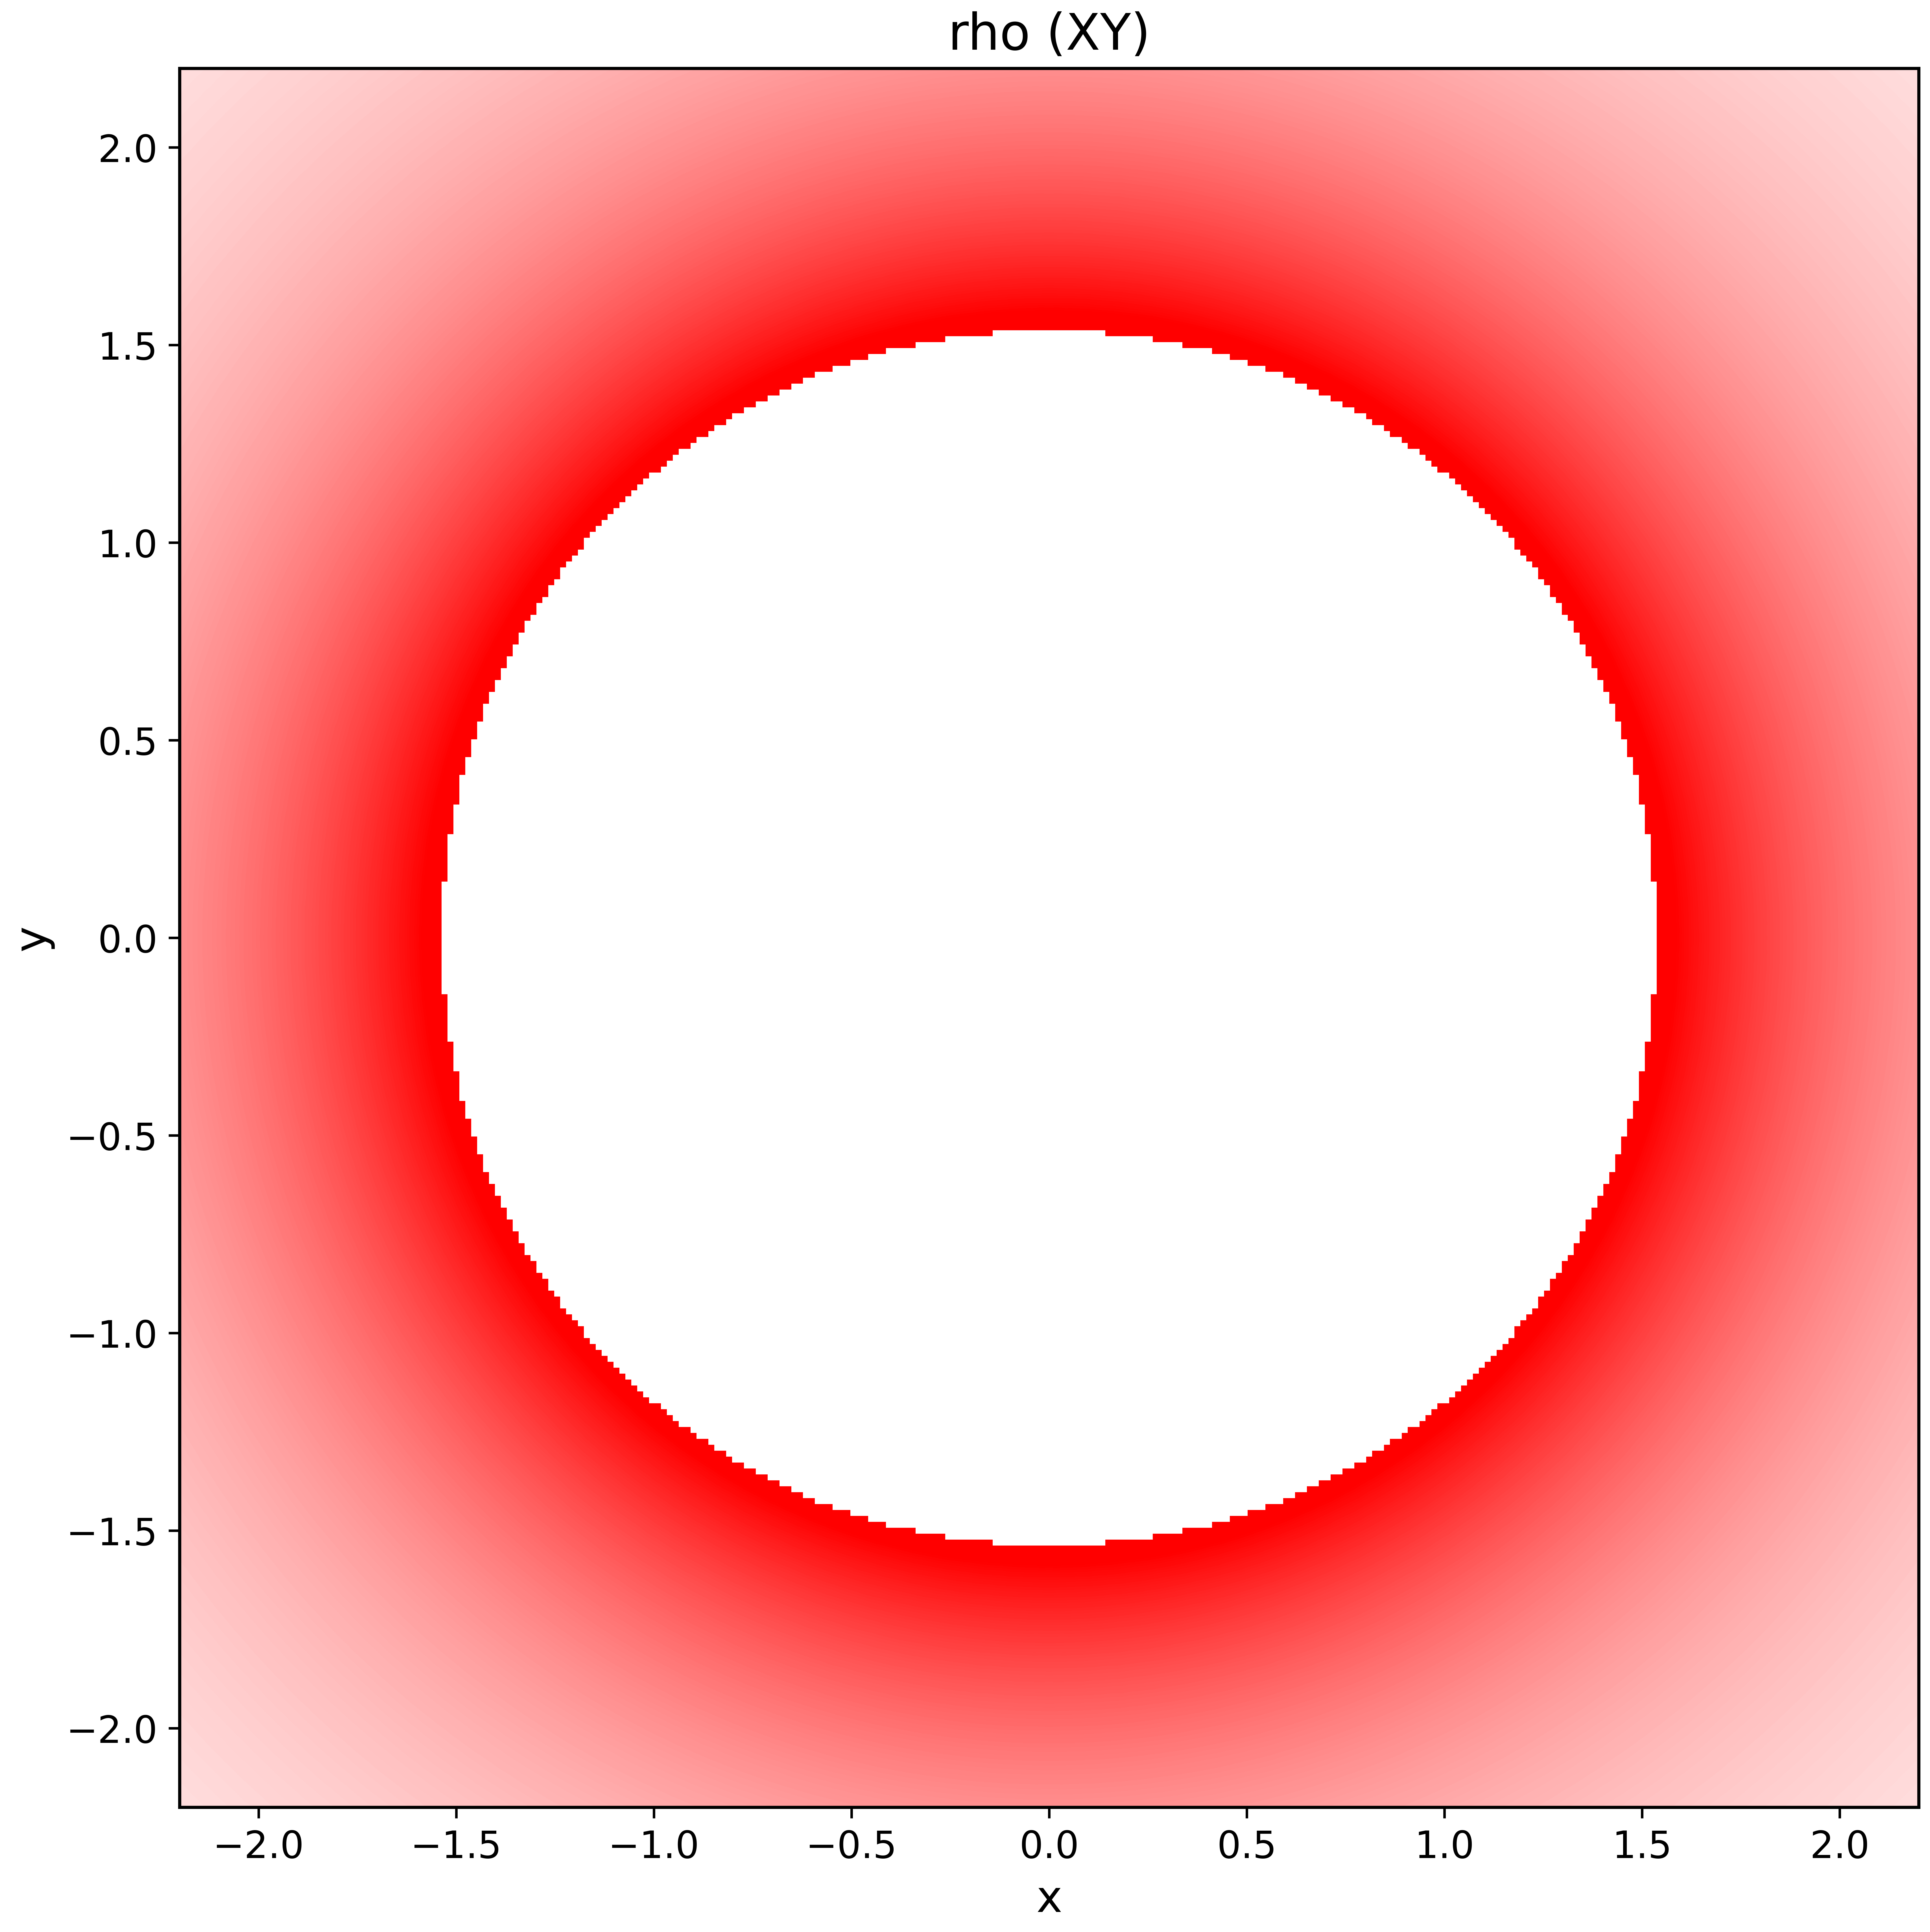
\includegraphics[width=\linewidth]{figures/domain_1_v_0p1_t_30p0_a0p970_b1p321_R00p000_XY_rho.png}
    \caption{Energy density \(\rho\) on the equatorial slice; the red annulus marks the positive-energy shell separating interior and exterior vacua.}
    \label{fig:d1-xy-rho}
  \end{subfigure}\hfill
  \begin{subfigure}[b]{0.46\textwidth}
    \centering
    \includegraphics[width=\linewidth]{figures/domain_1_v_0p1_t_30p0_a0p970_b1p321_R00p000_XY_WECmin.png}
    \caption{Minimum weak-energy--condition margin \(\mathrm{WEC}_{\min}\); the regenerated slice contains localized negative sectors rather than remaining everywhere non-negative, but the strongest residual obstruction still appears in the DEC diagnostic.}
    \label{fig:d1-xy-wecmin}
  \end{subfigure}

  \vspace{1ex}

  \begin{subfigure}[b]{0.46\textwidth}
    \centering
    \includegraphics[width=\linewidth]{figures/domain_1_v_0p1_t_30p0_a0p970_b1p321_R00p000_XY_NECmin.png}
    \caption{Minimum null-energy--condition margin \(\mathrm{NEC}_{\min}\), showing a localized deficit structure similar to the WEC diagnostic rather than a fully near-saturated shell.}
    \label{fig:d1-xy-necmin}
  \end{subfigure}

  \caption{Single-shell configuration, equatorial \(x\mbox{--}y\) slice at \(v=0.1\), \(t=30\).
  Throughout the field maps: \emph{blue} = negative (violation), \emph{white} = near zero (saturation), \emph{red} = positive (satisfied). See Table~\ref{tab:summary} for quantitative success fractions.}
  \label{fig:d1-xy-energy-A}
\end{figure}

%-----------------------------------------------------
% Single shell: Energy conditions, XY slice (2 panels)
%-----------------------------------------------------
\begin{figure}[htbp]
  \centering
  \begin{subfigure}[b]{0.46\textwidth}
    \centering
    \includegraphics[width=\linewidth]{figures/domain_1_v_0p1_t_30p0_a0p970_b1p321_R00p000_XY_DECmargin.png}
    \caption{DEC margin, highlighting a narrow blue ring where tangential stresses exceed \(\rho\) in magnitude while the density itself remains positive.}
    \label{fig:d1-xy-decmargin}
  \end{subfigure}\hfill
  \begin{subfigure}[b]{0.46\textwidth}
    \centering
    \includegraphics[width=\linewidth]{figures/domain_1_v_0p1_t_30p0_a0p970_b1p321_R00p000_XY_SEC.png}
    \caption{Strong-energy--condition \(\SEC=\rho+p_1+p_2+p_3\) on the equatorial slice; the regenerated trace is sign-changing, although it remains less restrictive in aggregate than the DEC margin.}
    \label{fig:d1-xy-sec}
  \end{subfigure}
  \caption{Single-shell configuration, equatorial slice:
  diagnostics that identify the dominant residual constraint as the \DEC\ rather than the \WEC/\NEC. Quantitative success fractions and minimum margins are reported in Table~\ref{tab:summary} and Sec.~\ref{sec:quantitative}.}
  \label{fig:d1-xy-energy-B}
\end{figure}

%-----------------------------------------------------
% Single shell: Energy conditions, XZ slice (3 panels)
%-----------------------------------------------------
\begin{figure}[htbp]
  \centering
  \begin{subfigure}[b]{0.46\textwidth}
    \centering
    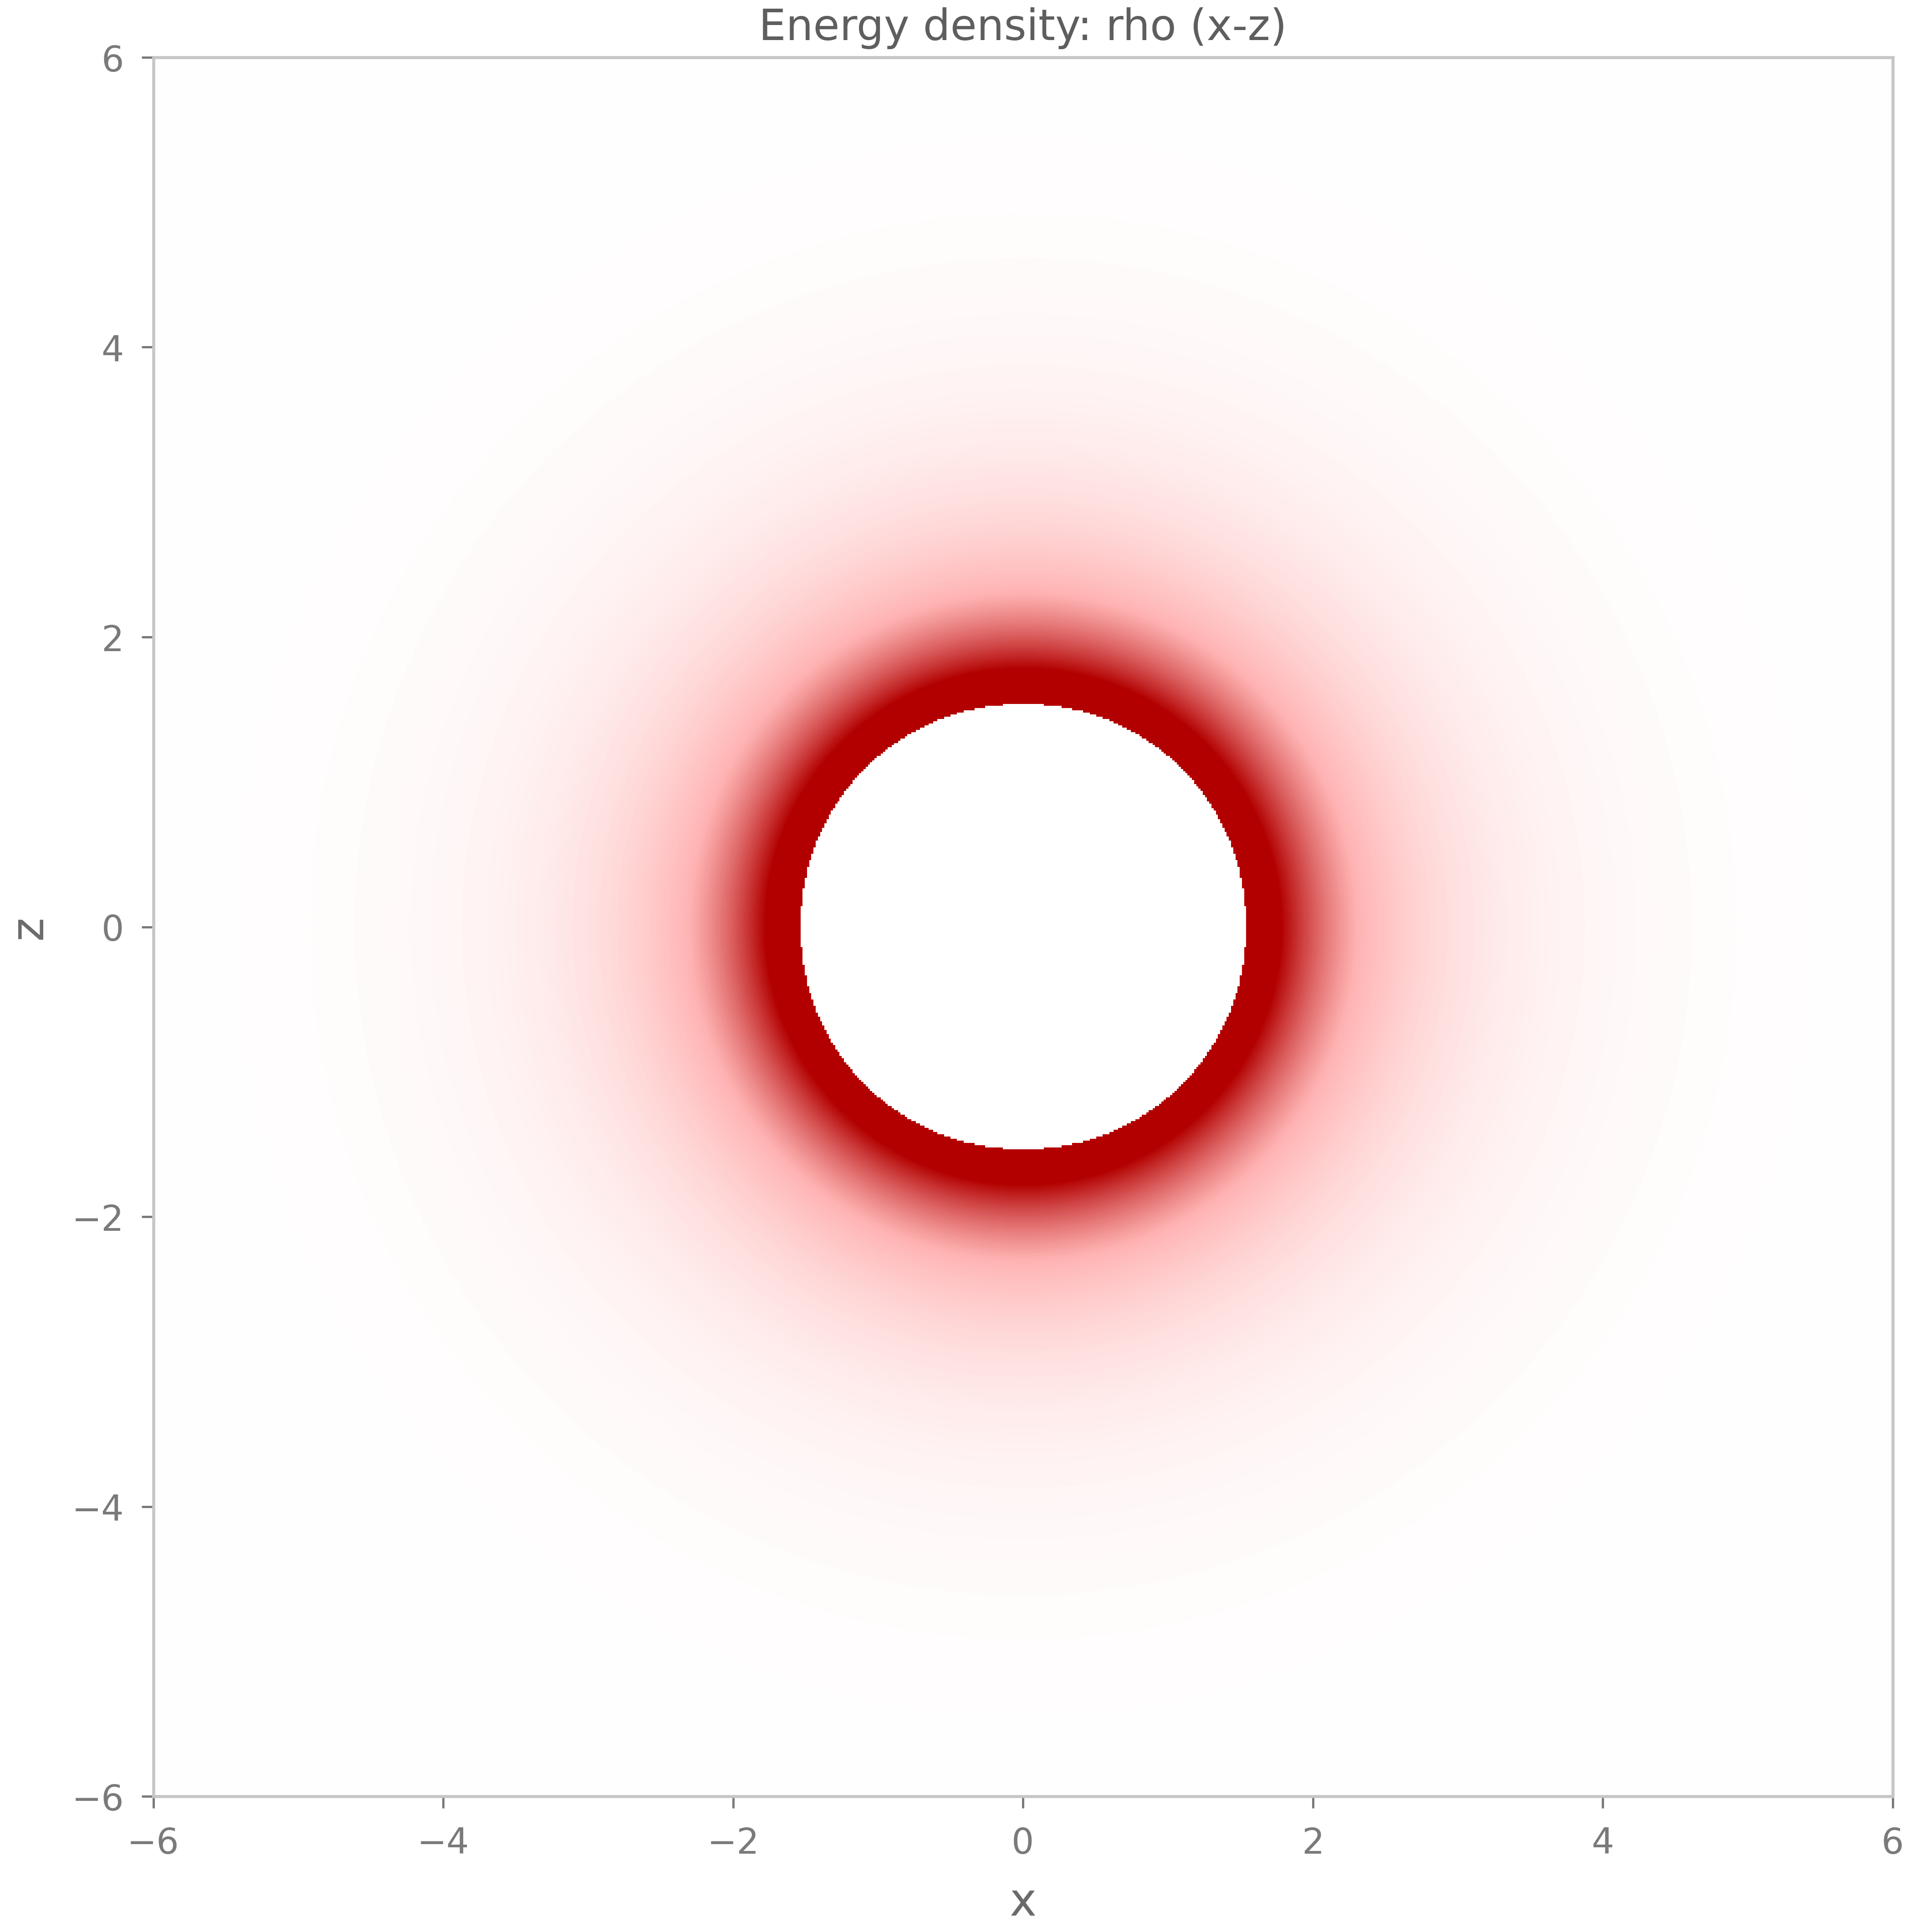
\includegraphics[width=\linewidth]{figures/domain_1_v_0p1_t_30p0_a0p970_b1p321_R00p000_XZ_rho.png}
    \caption{Energy density \(\rho\) on the meridional \(x\mbox{--}z\) slice; the thin red annulus shows the same single-shell structure in cross-section.}
    \label{fig:d1-xz-rho}
  \end{subfigure}\hfill
  \begin{subfigure}[b]{0.46\textwidth}
    \centering
    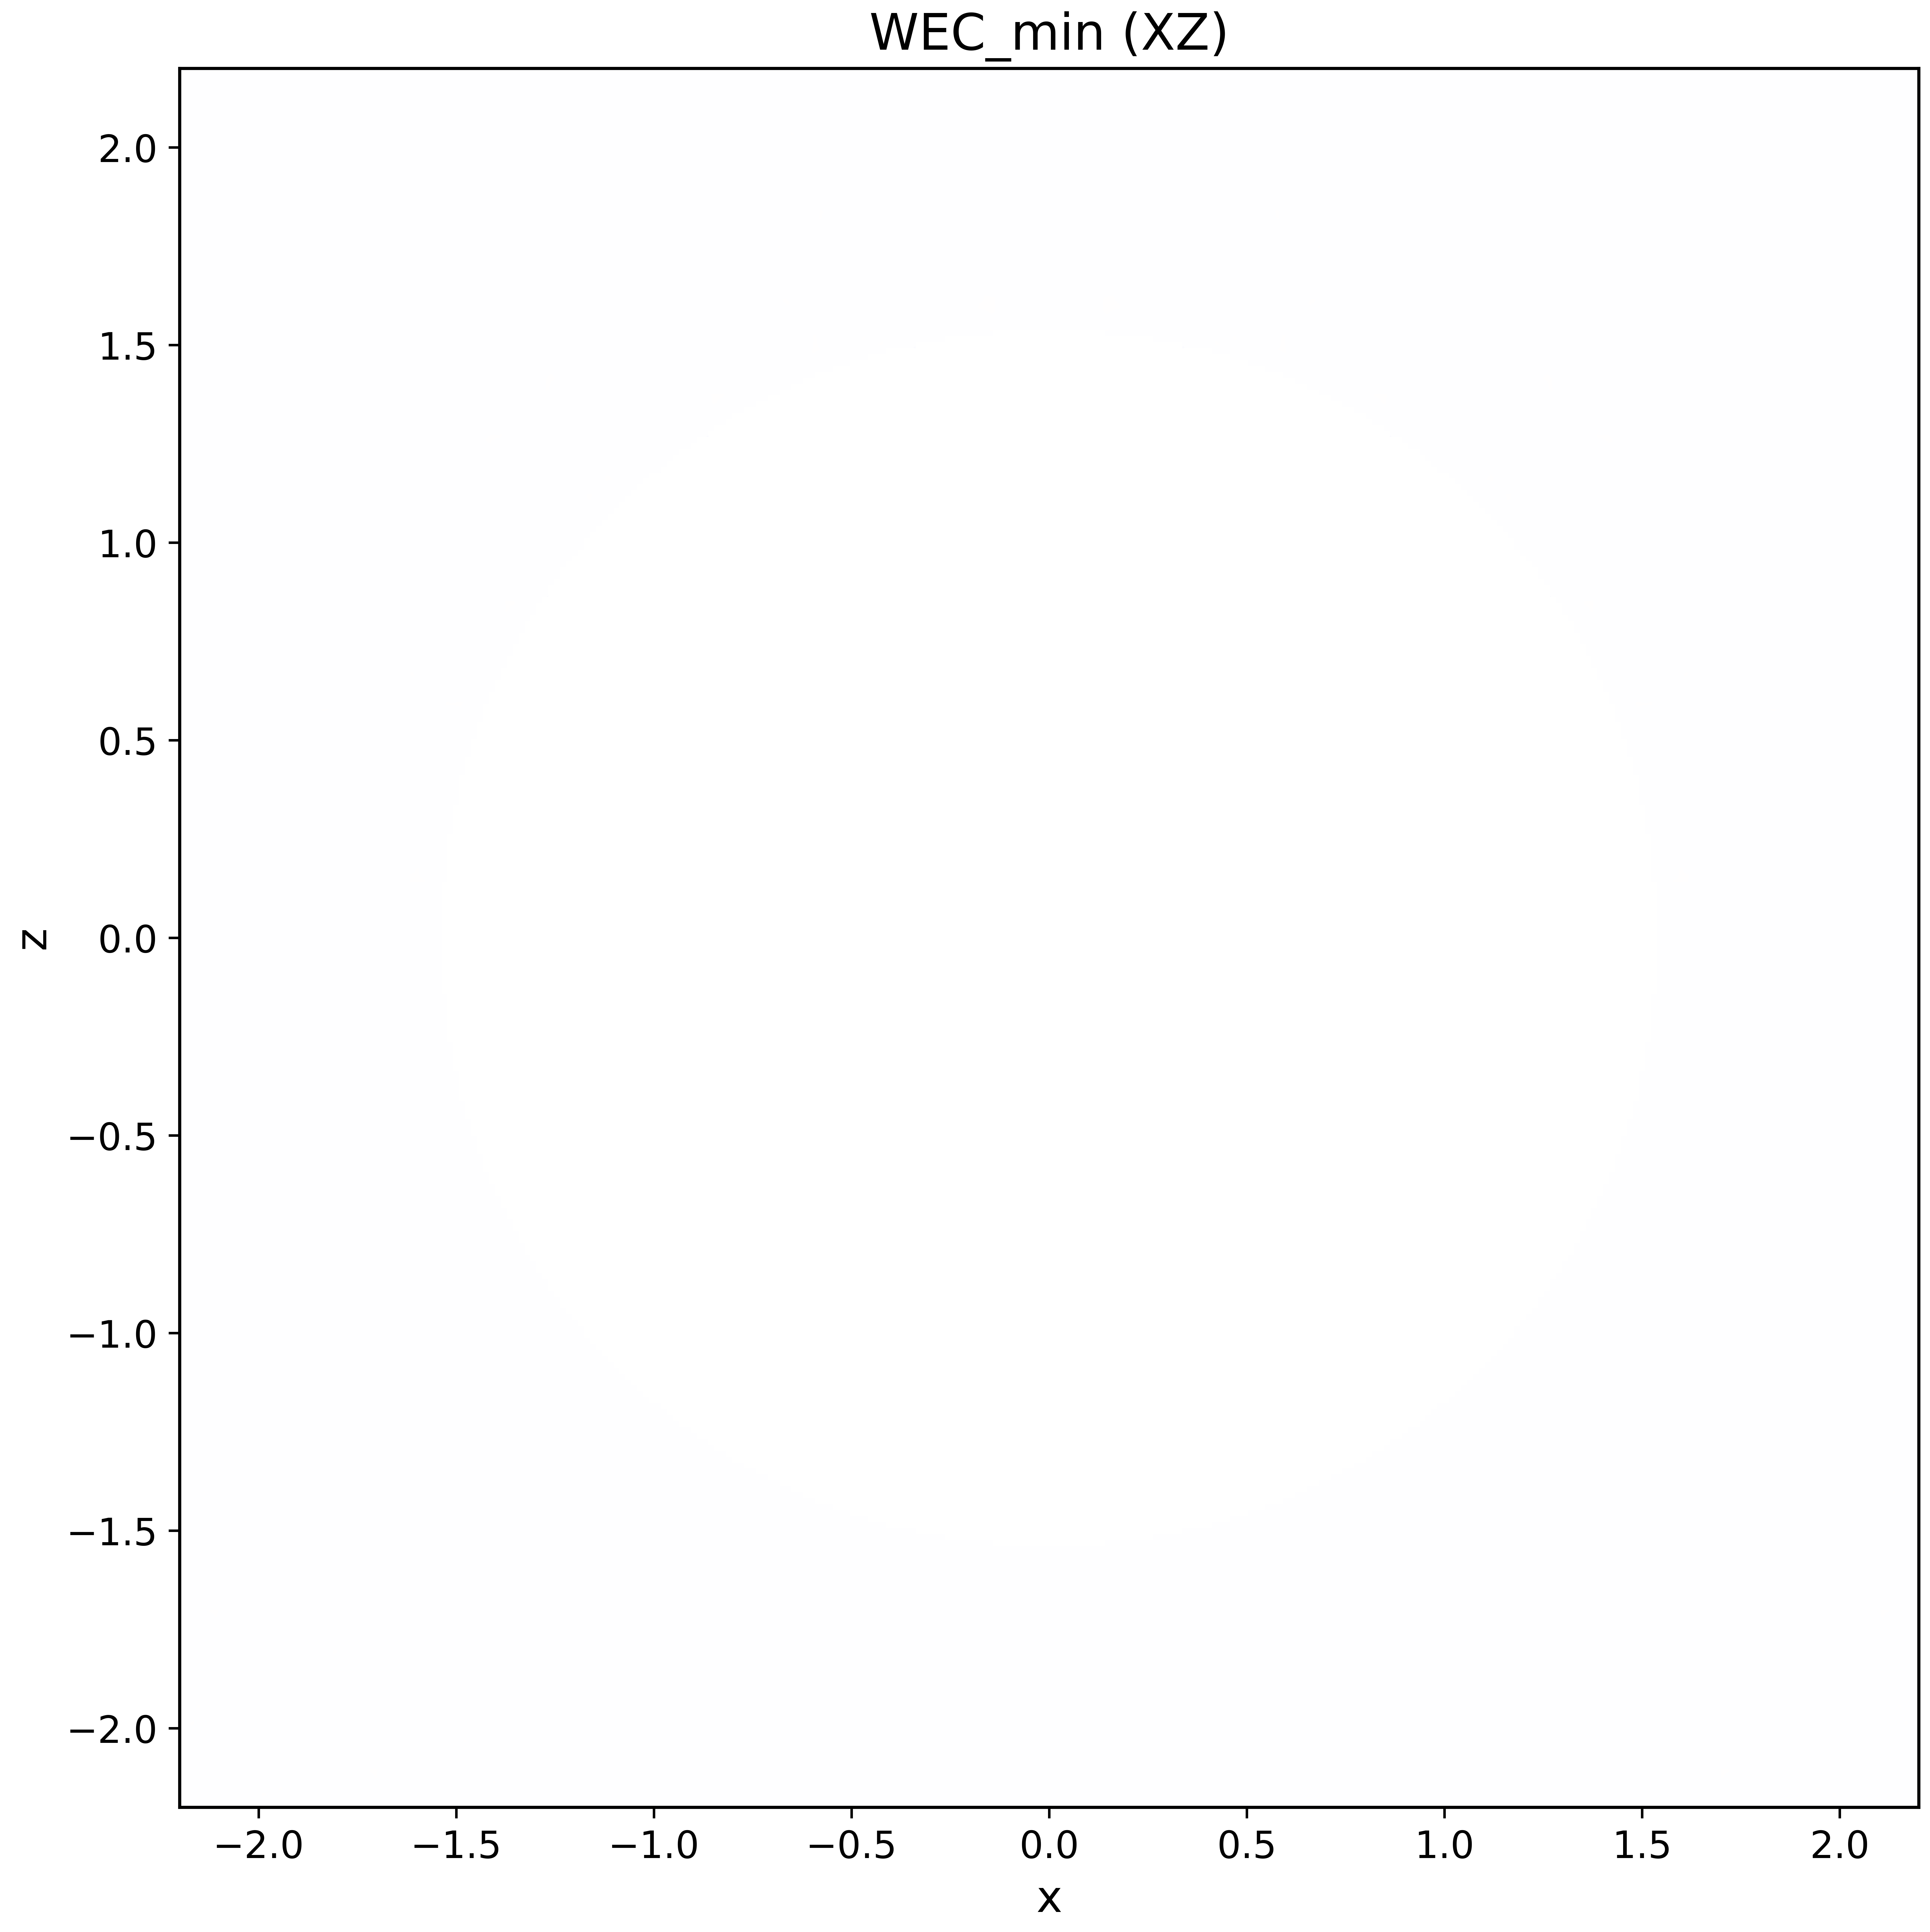
\includegraphics[width=\linewidth]{figures/domain_1_v_0p1_t_30p0_a0p970_b1p321_R00p000_XZ_WECmin.png}
    \caption{\(\mathrm{WEC}_{\min}\) on the meridional slice; the regenerated map shows localized negative sectors rather than a uniformly near-zero shell.}
    \label{fig:d1-xz-wecmin}
  \end{subfigure}

  \vspace{1ex}

  \begin{subfigure}[b]{0.46\textwidth}
    \centering
    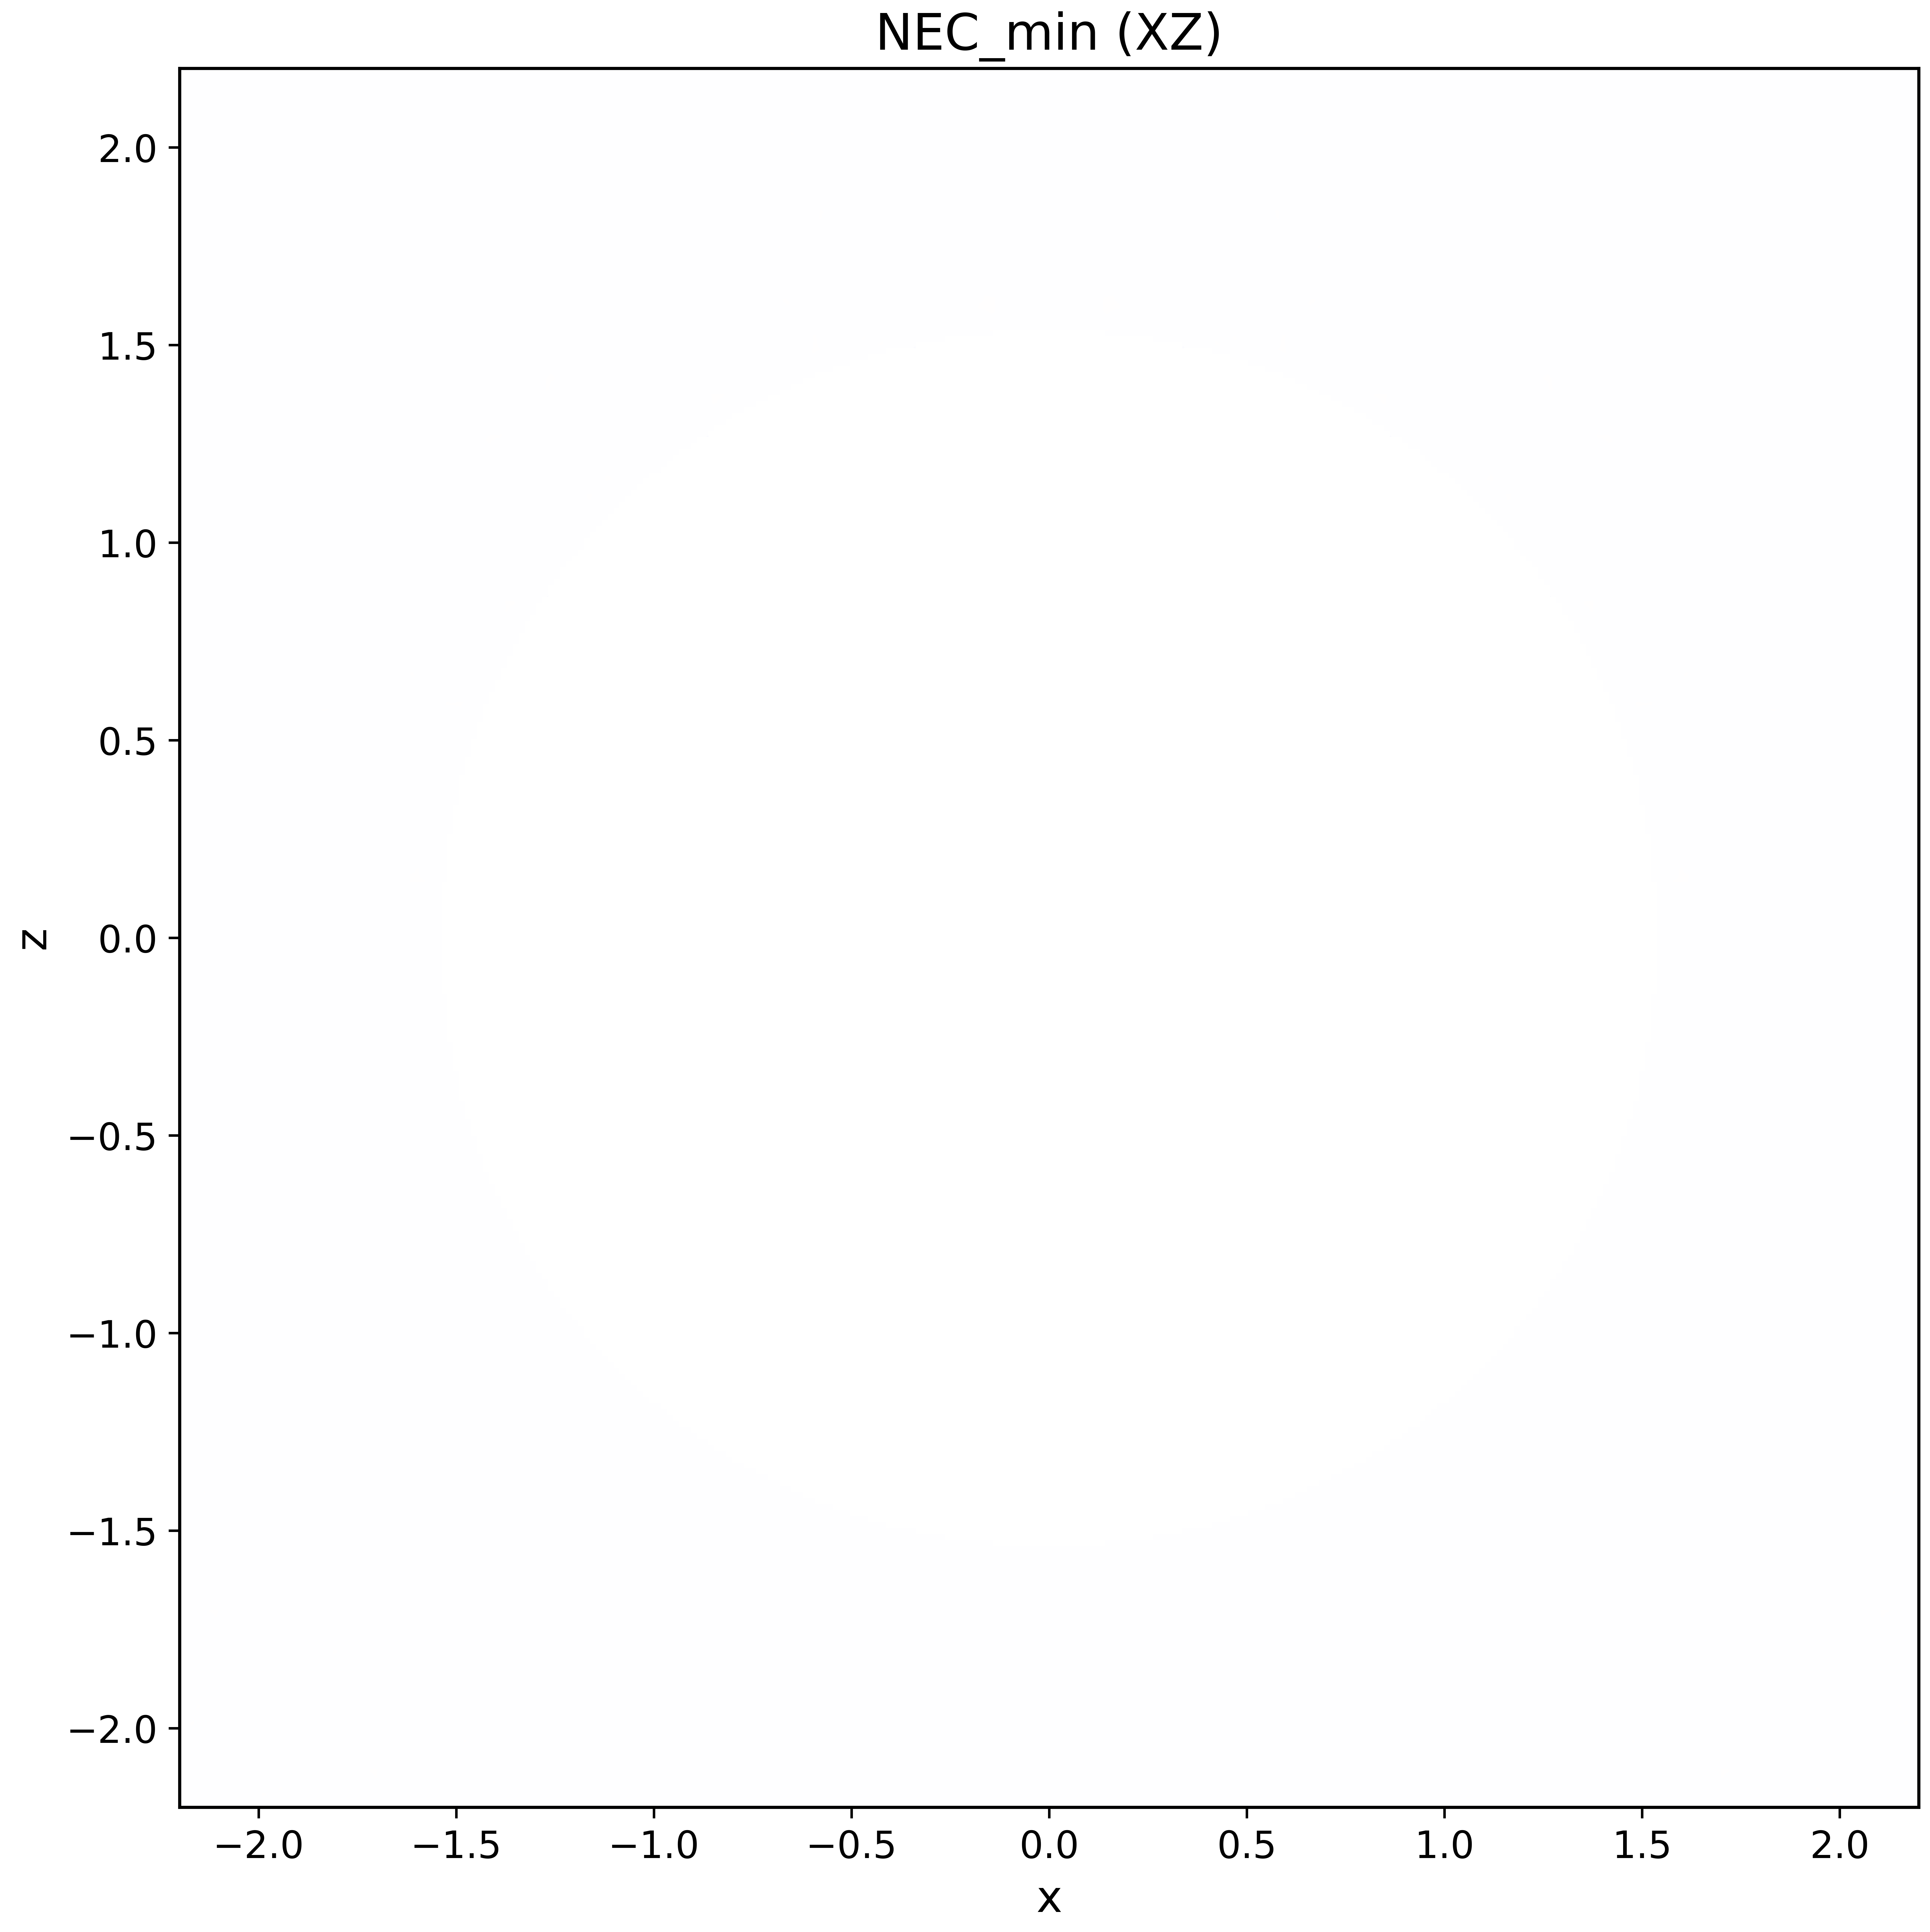
\includegraphics[width=\linewidth]{figures/domain_1_v_0p1_t_30p0_a0p970_b1p321_R00p000_XZ_NECmin.png}
    \caption{\(\mathrm{NEC}_{\min}\), showing the same localized deficit structure as the WEC diagnostic on the meridional slice.}
    \label{fig:d1-xz-necmin}
  \end{subfigure}

  \caption{Single-shell configuration, meridional \(x\mbox{--}z\) slice:
  density and minimum \WEC/\NEC\ margins, complementary to the equatorial view in Fig.~\ref{fig:d1-xy-energy-A}. See Table~\ref{tab:summary} for quantitative values.}
  \label{fig:d1-xz-energy-A}
\end{figure}

%-----------------------------------------------------
% Single shell: Energy conditions, XZ slice (2 panels)
%-----------------------------------------------------
\begin{figure}[htbp]
  \centering
  \begin{subfigure}[b]{0.46\textwidth}
    \centering
    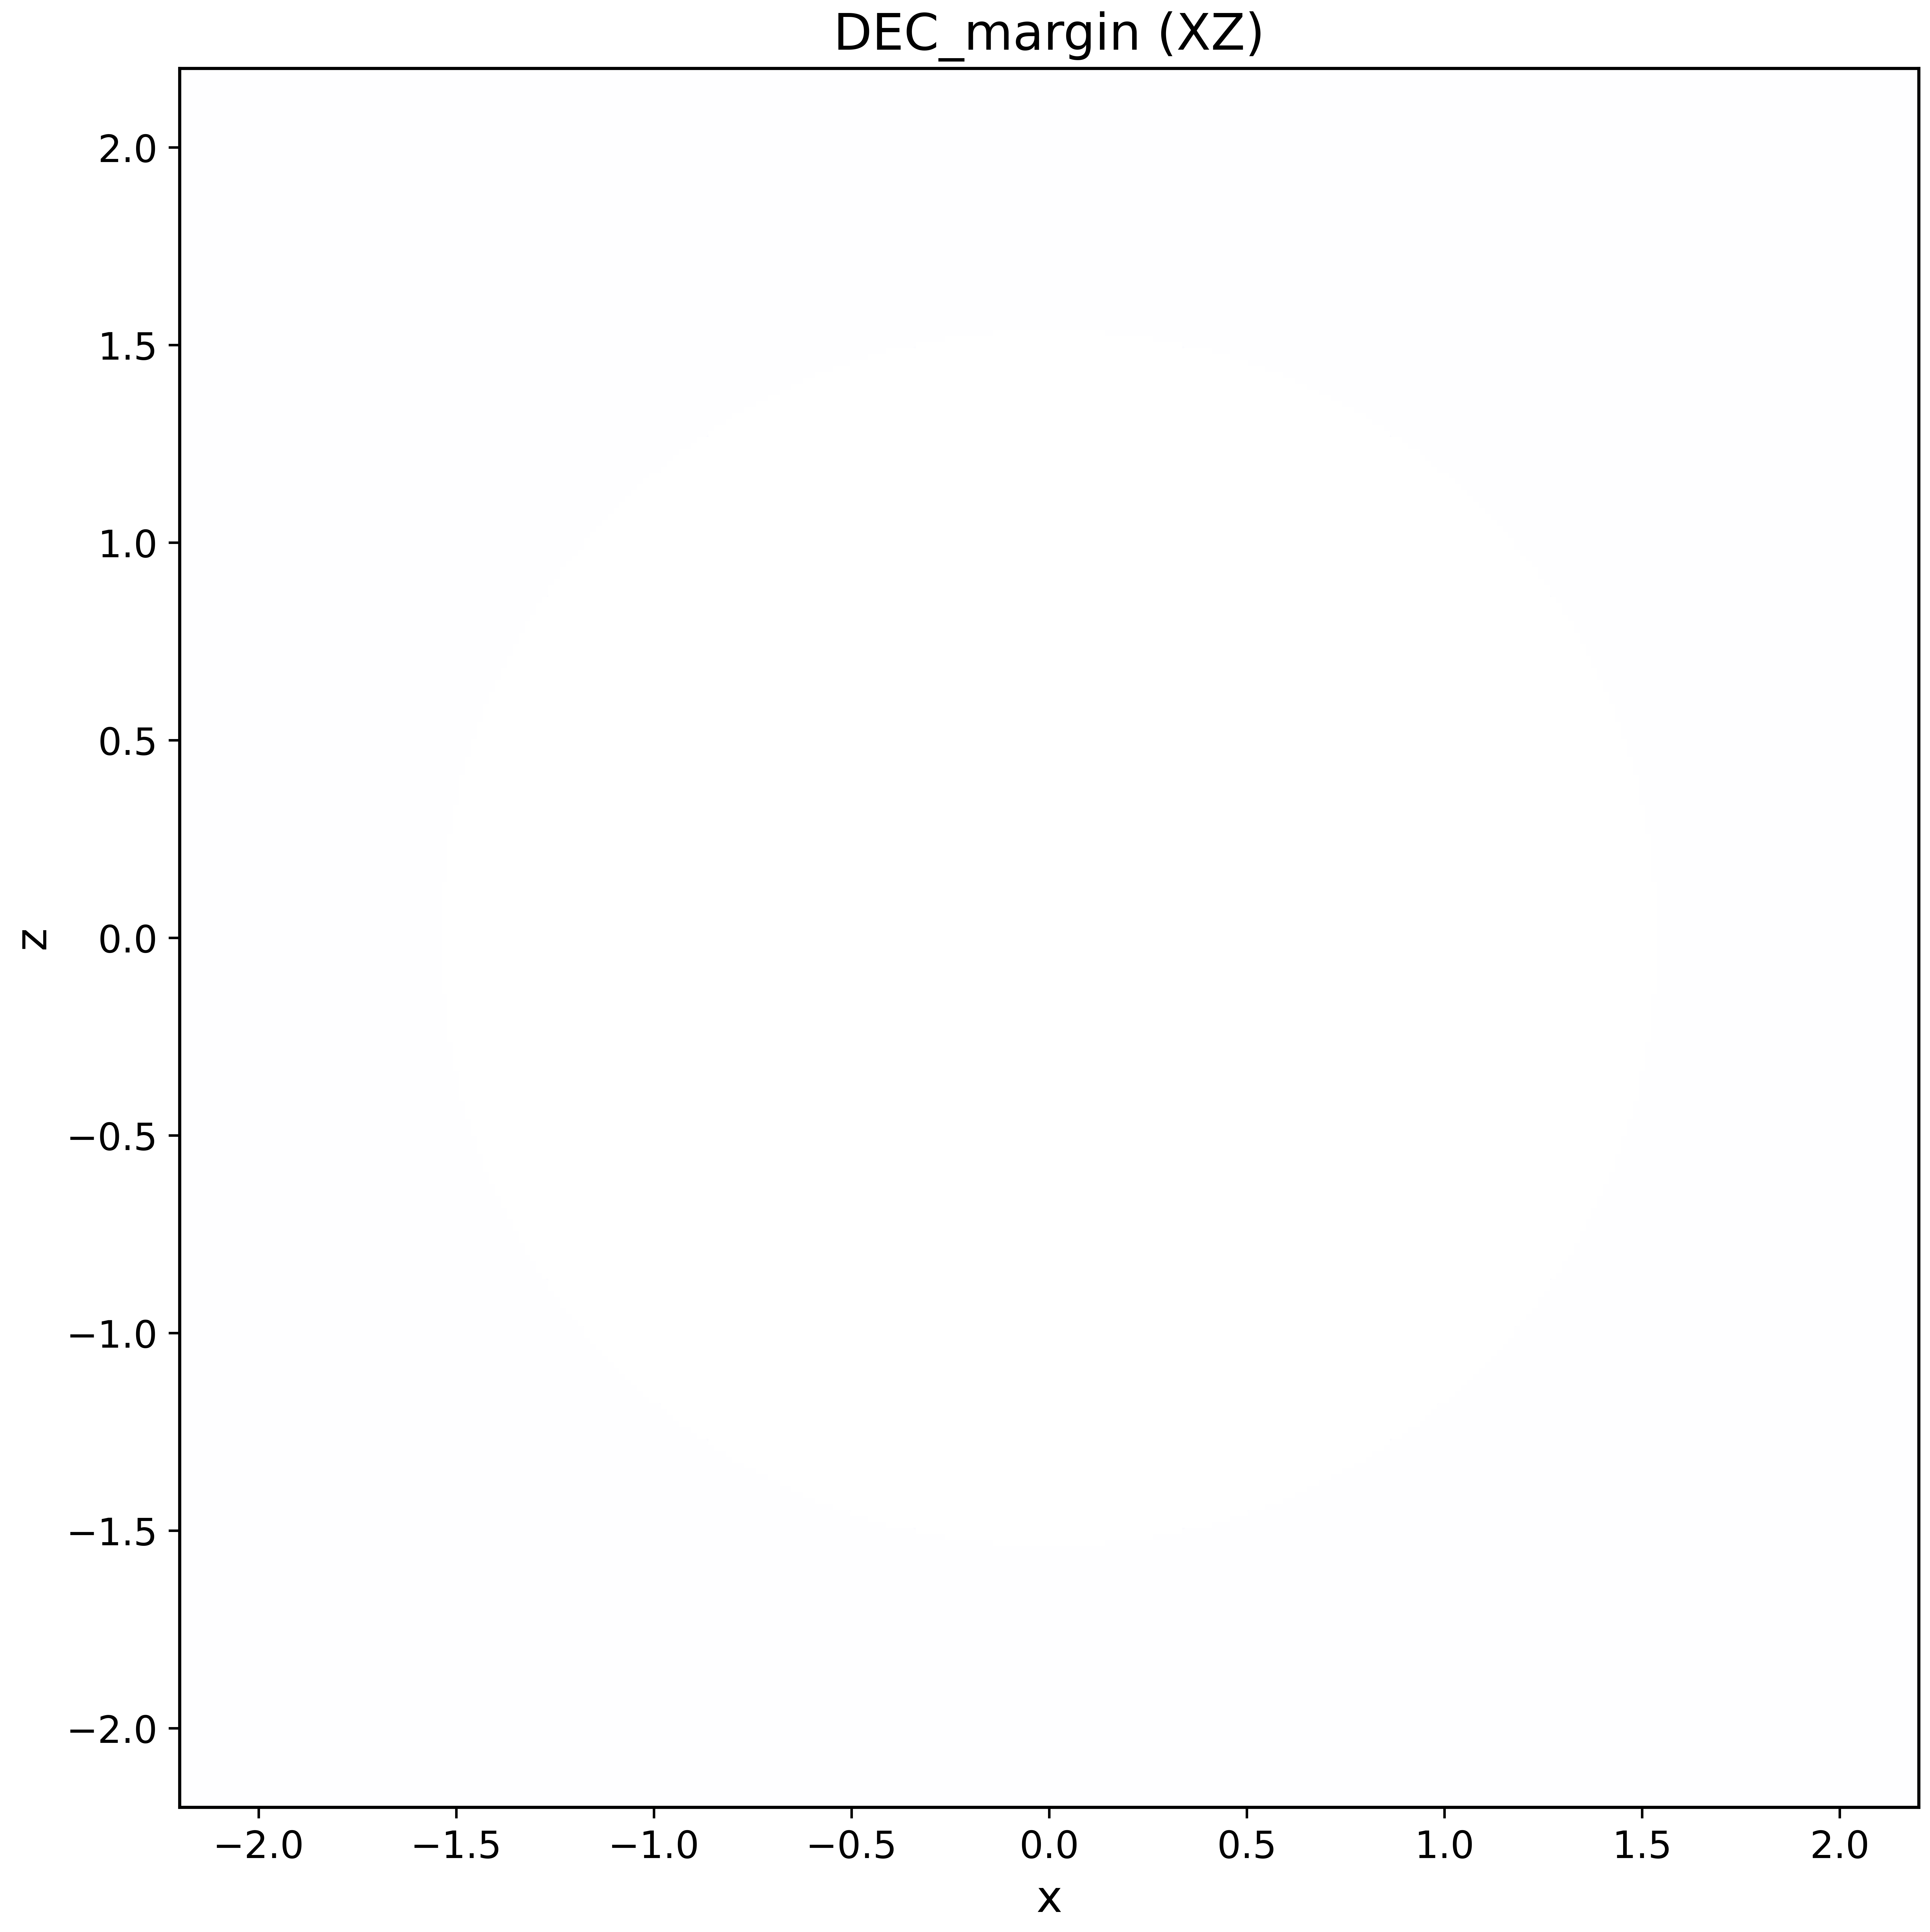
\includegraphics[width=\linewidth]{figures/domain_1_v_0p1_t_30p0_a0p970_b1p321_R00p000_XZ_DECmargin.png}
    \caption{DEC margin, again exhibiting a thin ring of violation closely aligned with the shell interfaces.}
    \label{fig:d1-xz-decmargin}
  \end{subfigure}\hfill
  \begin{subfigure}[b]{0.46\textwidth}
    \centering
    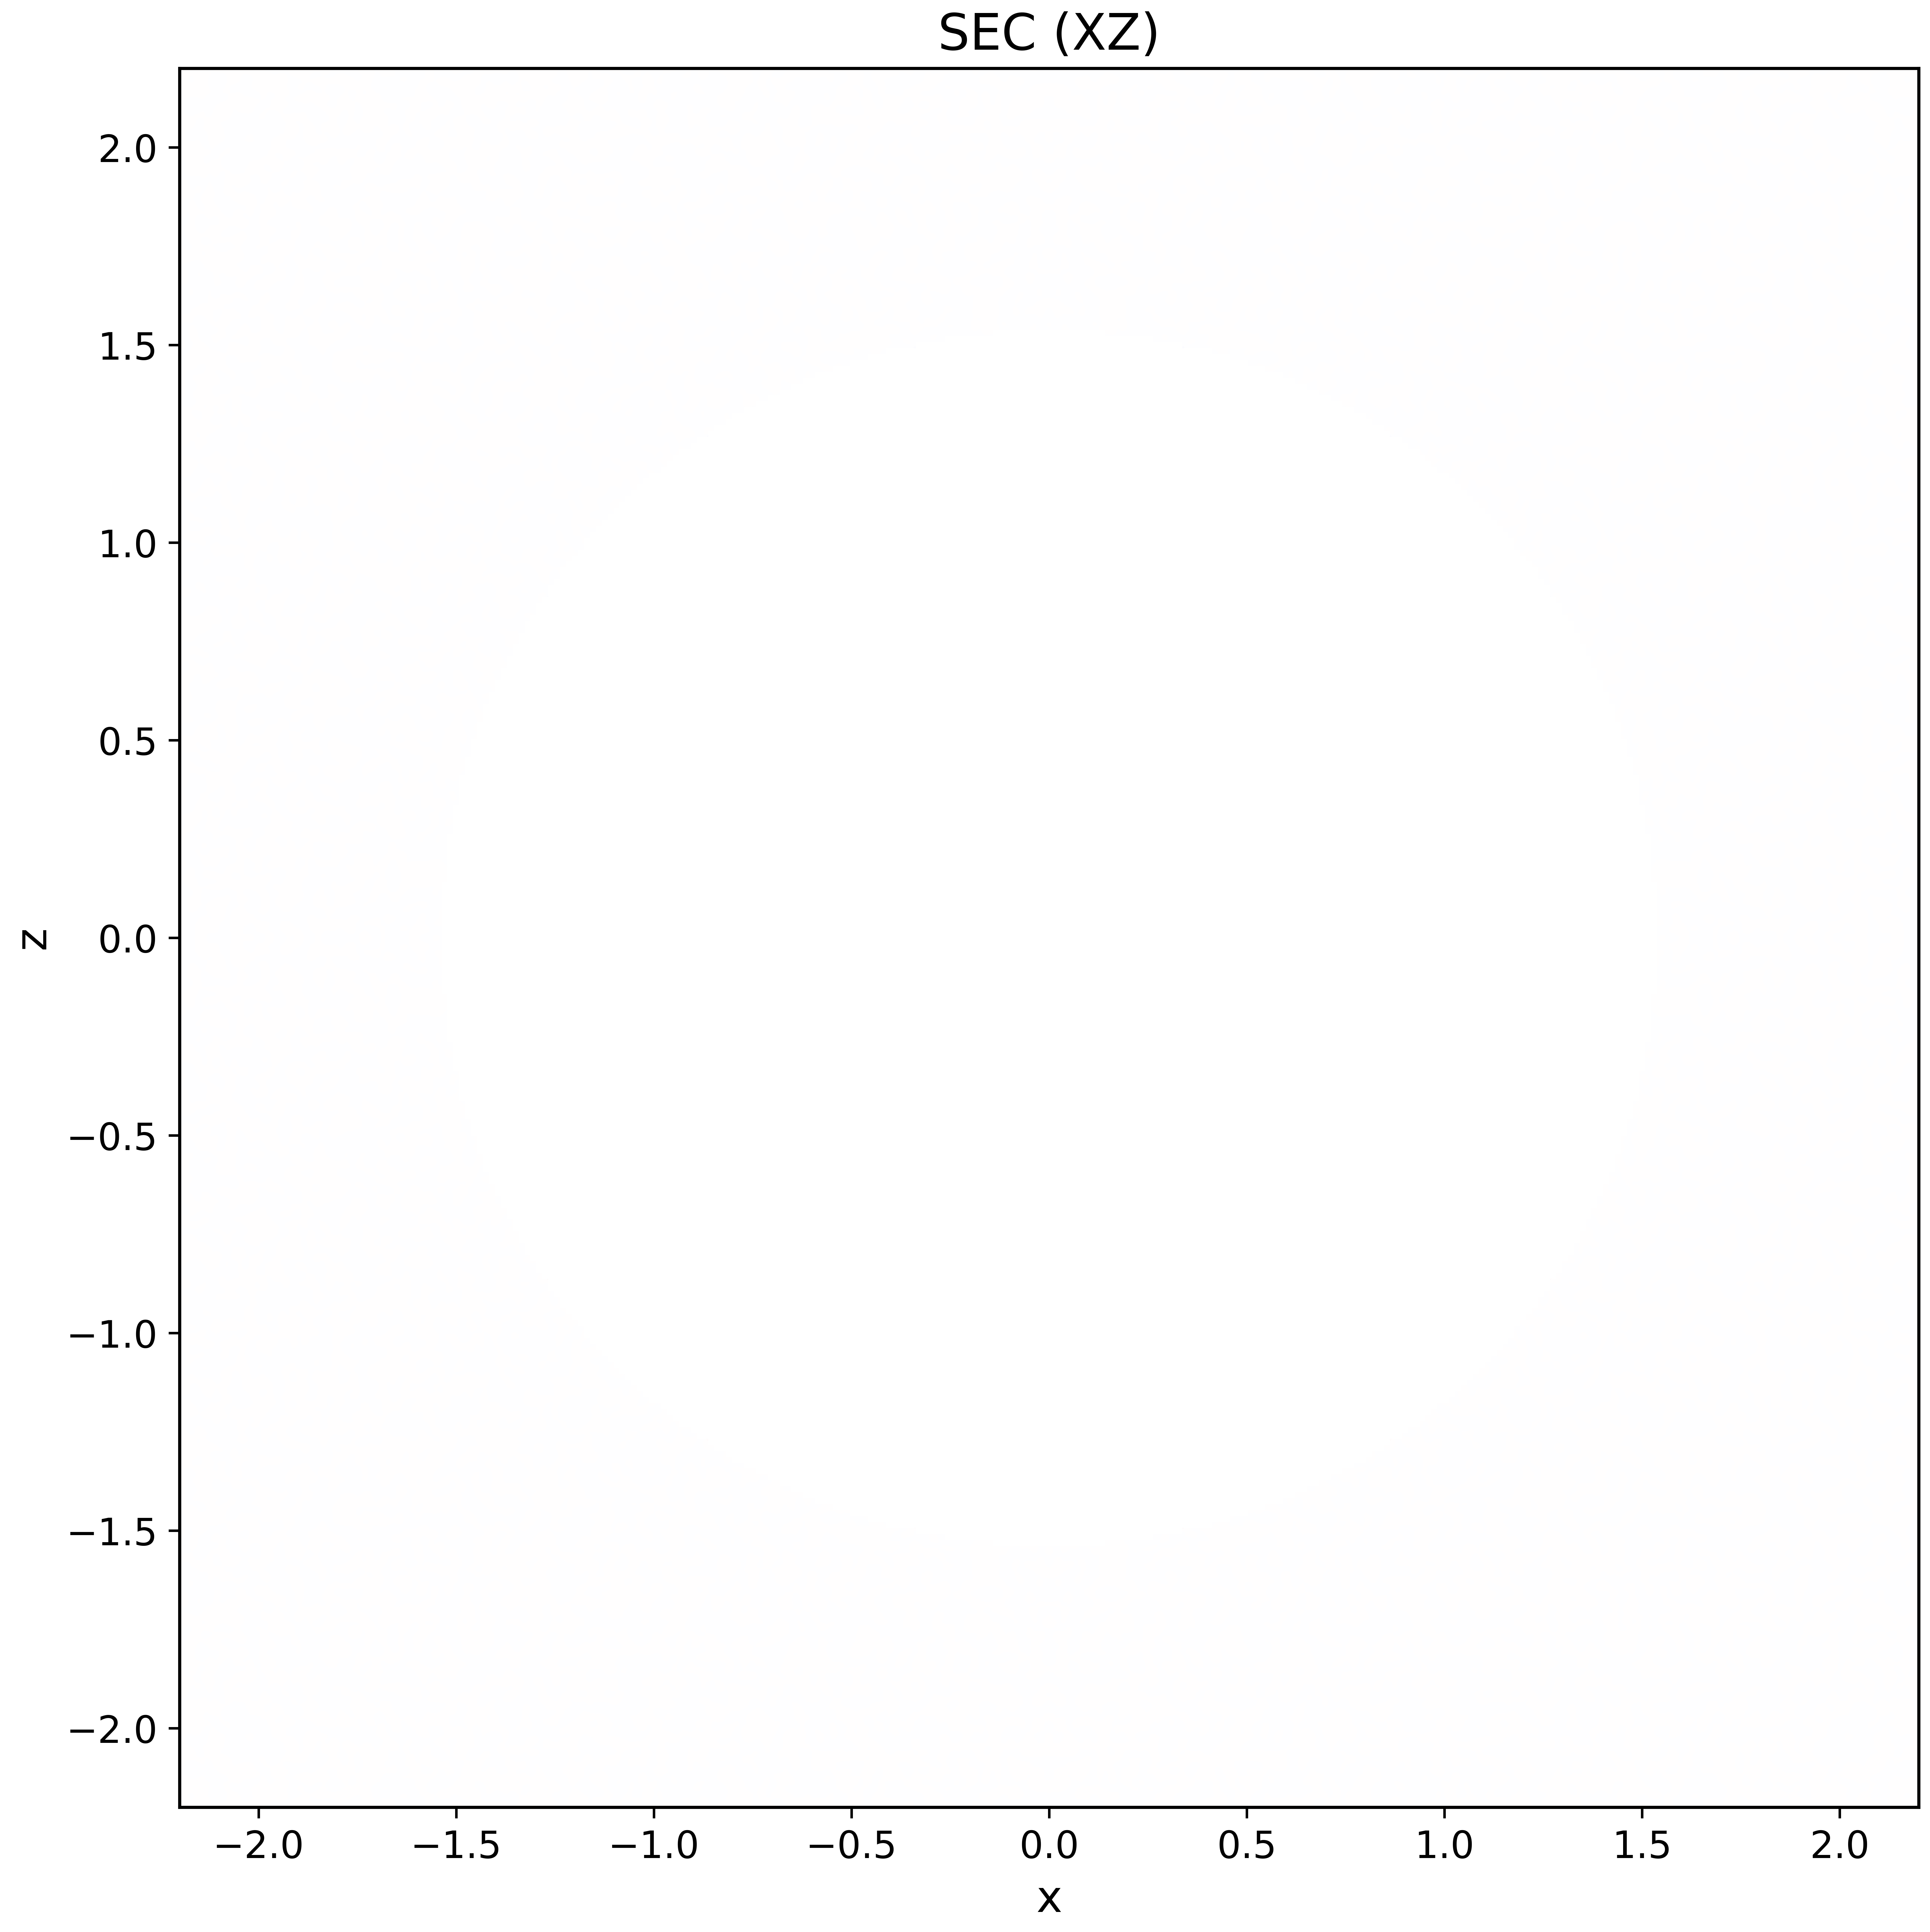
\includegraphics[width=\linewidth]{figures/domain_1_v_0p1_t_30p0_a0p970_b1p321_R00p000_XZ_SEC.png}
    \caption{\(\SEC\) on the meridional slice; the regenerated trace is mixed rather than uniformly positive, but its aggregate success fraction still exceeds the DEC success fraction.}
    \label{fig:d1-xz-sec}
  \end{subfigure}

  \caption{Single-shell configuration, meridional slice:
  \DEC\ and \SEC\ diagnostics revealing that residual stress anisotropies are tightly localized.}
  \label{fig:d1-xz-energy-B}
\end{figure}

%-----------------------------------------------------
% Double shell: Energy conditions, XY slice (3 panels)
%-----------------------------------------------------
\begin{figure}[htbp]
  \centering
  \begin{subfigure}[b]{0.46\textwidth}
    \centering
    
\includegraphics[width=\linewidth]{figures/domain_2_v_0p1_t_30p0_a1p848_b1p135_R01p292_XY_rho.png}
    \caption{Energy density \(\rho\) on the equatorial slice for the double-shell seed; the positive-energy region now spans a broader annulus.}
    \label{fig:d2-xy-rho}
  \end{subfigure}\hfill
  \begin{subfigure}[b]{0.46\textwidth}
    \centering
    
\includegraphics[width=\linewidth]{figures/domain_2_v_0p1_t_30p0_a1p848_b1p135_R01p292_XY_WECmin.png}
    \caption{\(\mathrm{WEC}_{\min}\), showing a central blue region and inner-interface band where the WEC is violated while the outer shell remains close to saturation.}
    \label{fig:d2-xy-wecmin}
  \end{subfigure}

  \vspace{1ex}

  \begin{subfigure}[b]{0.46\textwidth}
    \centering
    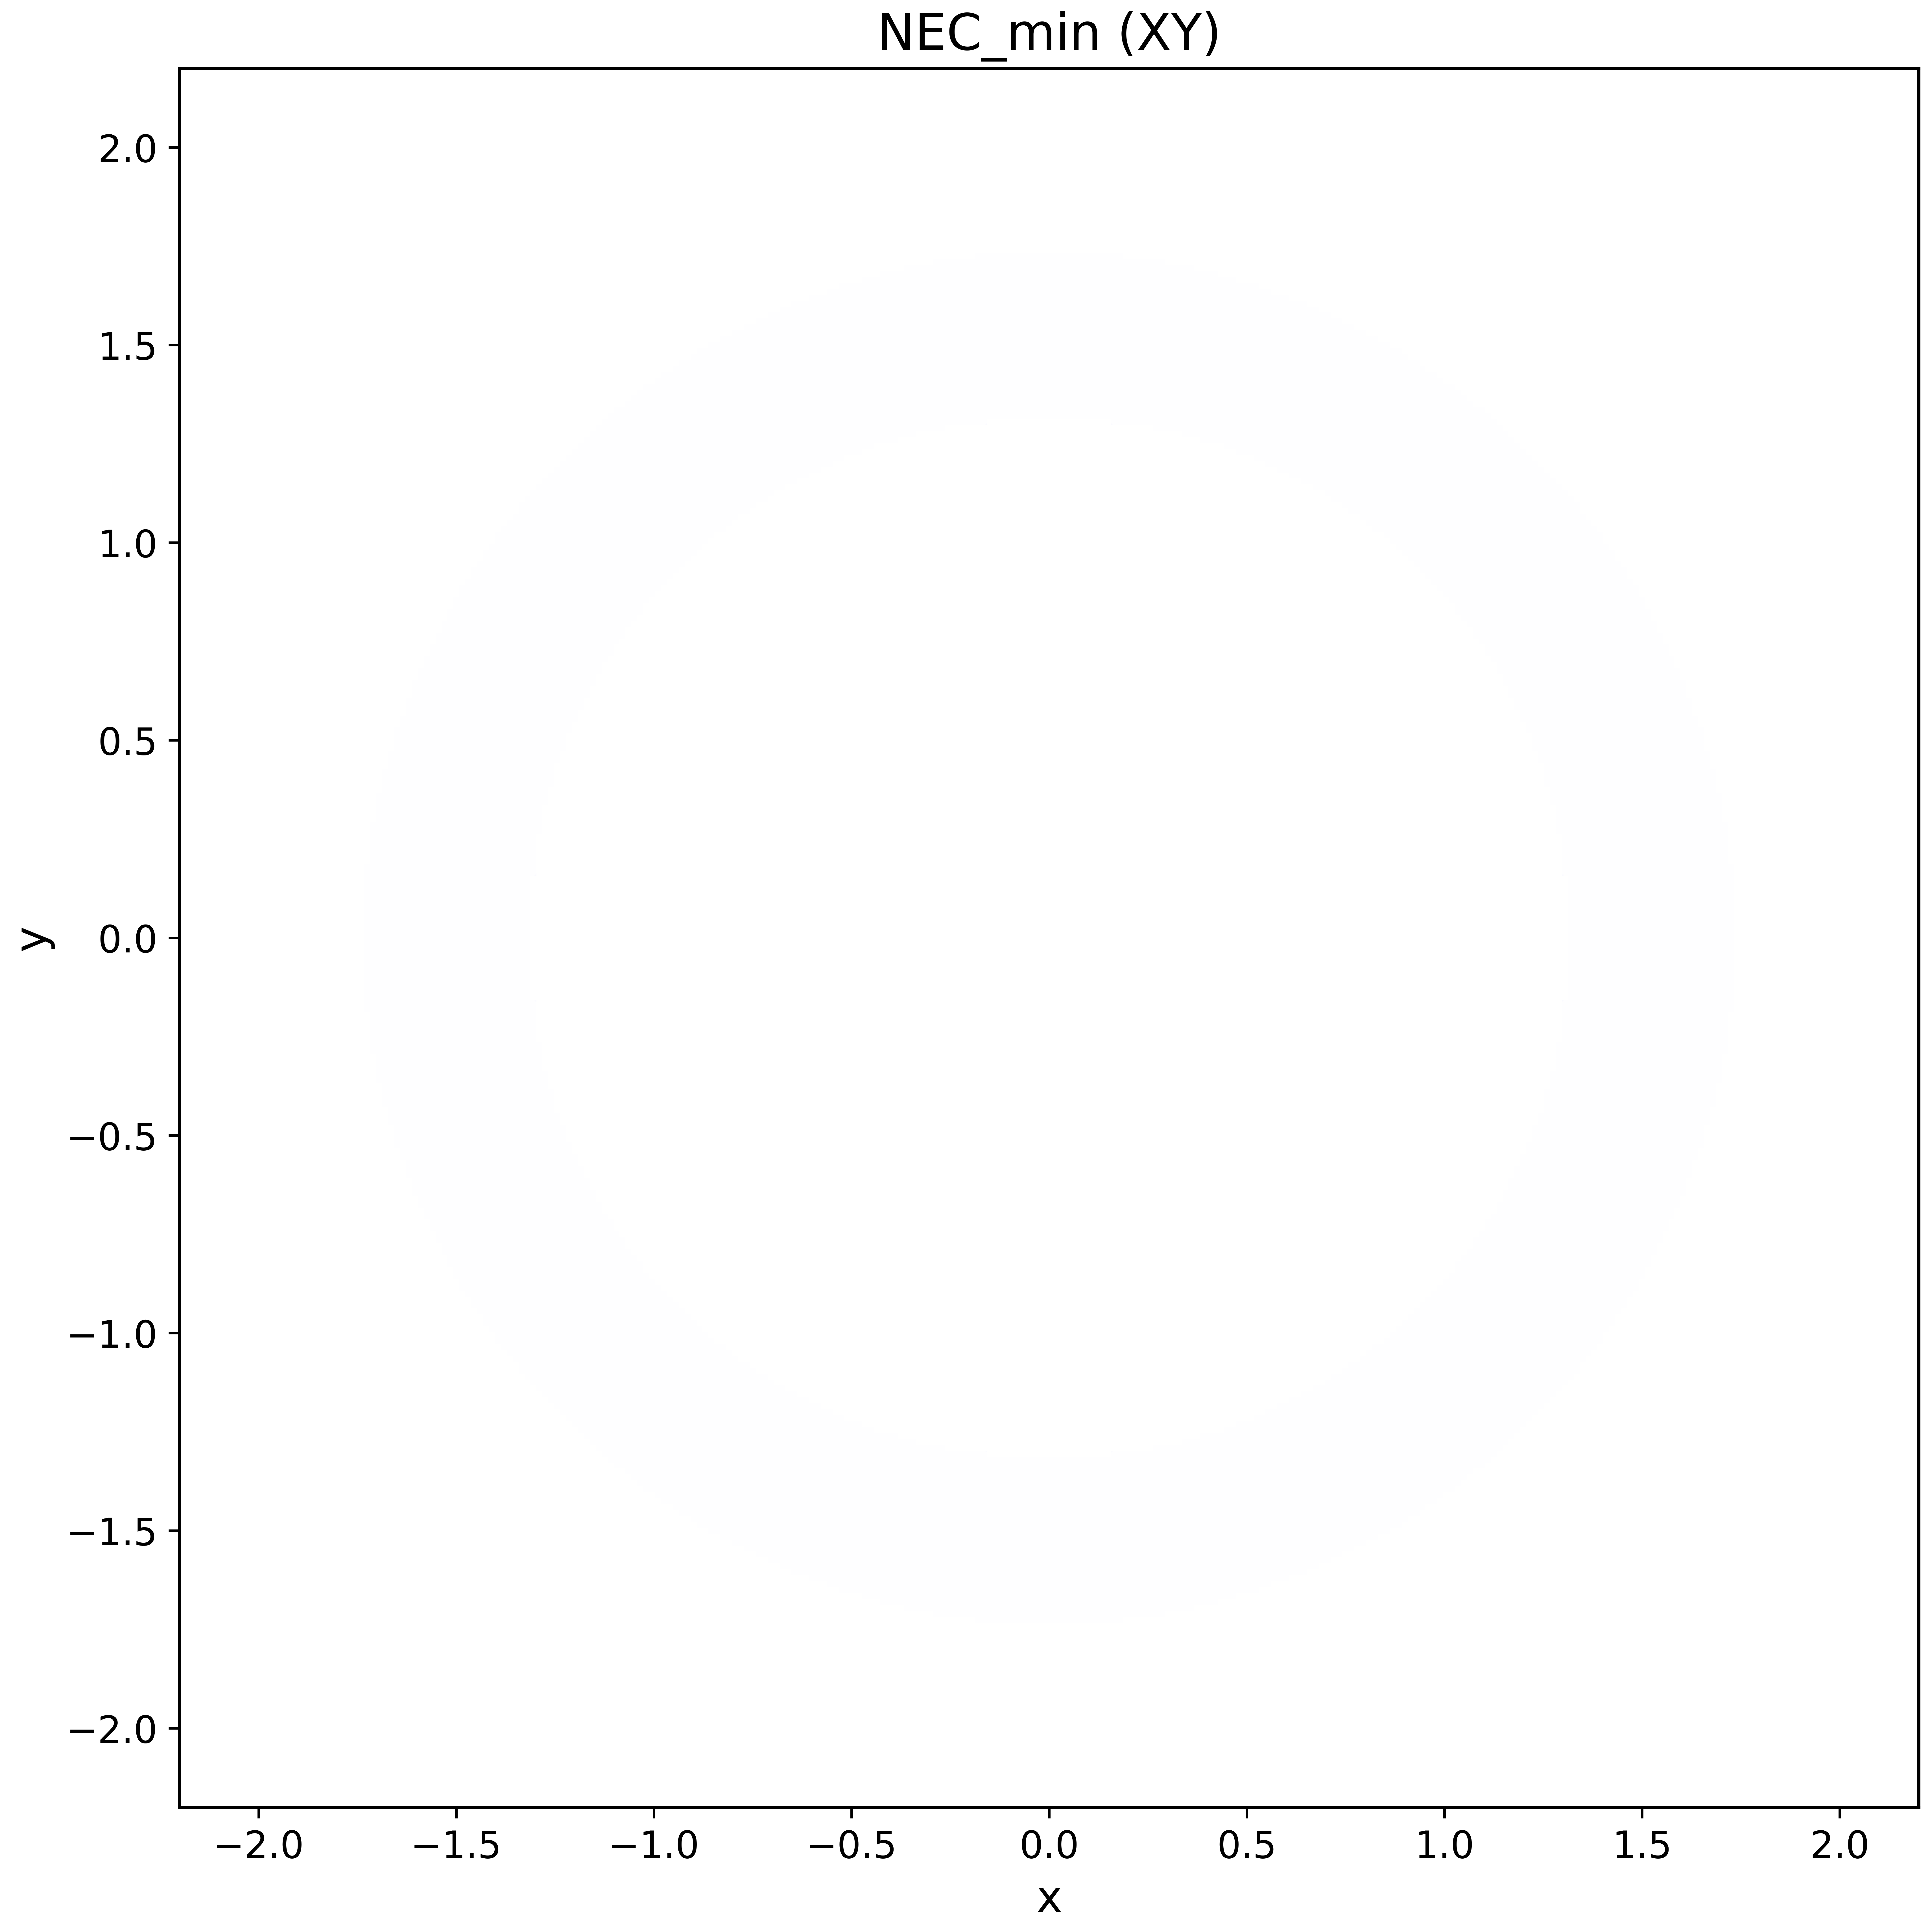
\includegraphics[width=\linewidth]{figures/domain_2_v_0p1_t_30p0_a1p848_b1p135_R01p292_XY_NECmin.png}
    \caption{\(\mathrm{NEC}_{\min}\), with a similar central deficit pattern, indicating that the inner vacuum interface is the main source of WEC/NEC violations.}
    \label{fig:d2-xy-necmin}
  \end{subfigure}

  \caption{Double-shell configuration, equatorial \(x\mbox{--}y\) slice:
  density and minimum \WEC/\NEC\ margins, illustrating how the extra interface changes where violations concentrate. See Table~\ref{tab:summary} for quantitative success fractions and minimum margins.}
  \label{fig:d2-xy-energy-A}
\end{figure}

%-----------------------------------------------------
% Double shell: Energy conditions, XY slice (2 panels)
%-----------------------------------------------------
\begin{figure}[htbp]
  \centering
  \begin{subfigure}[b]{0.46\textwidth}
    \centering
    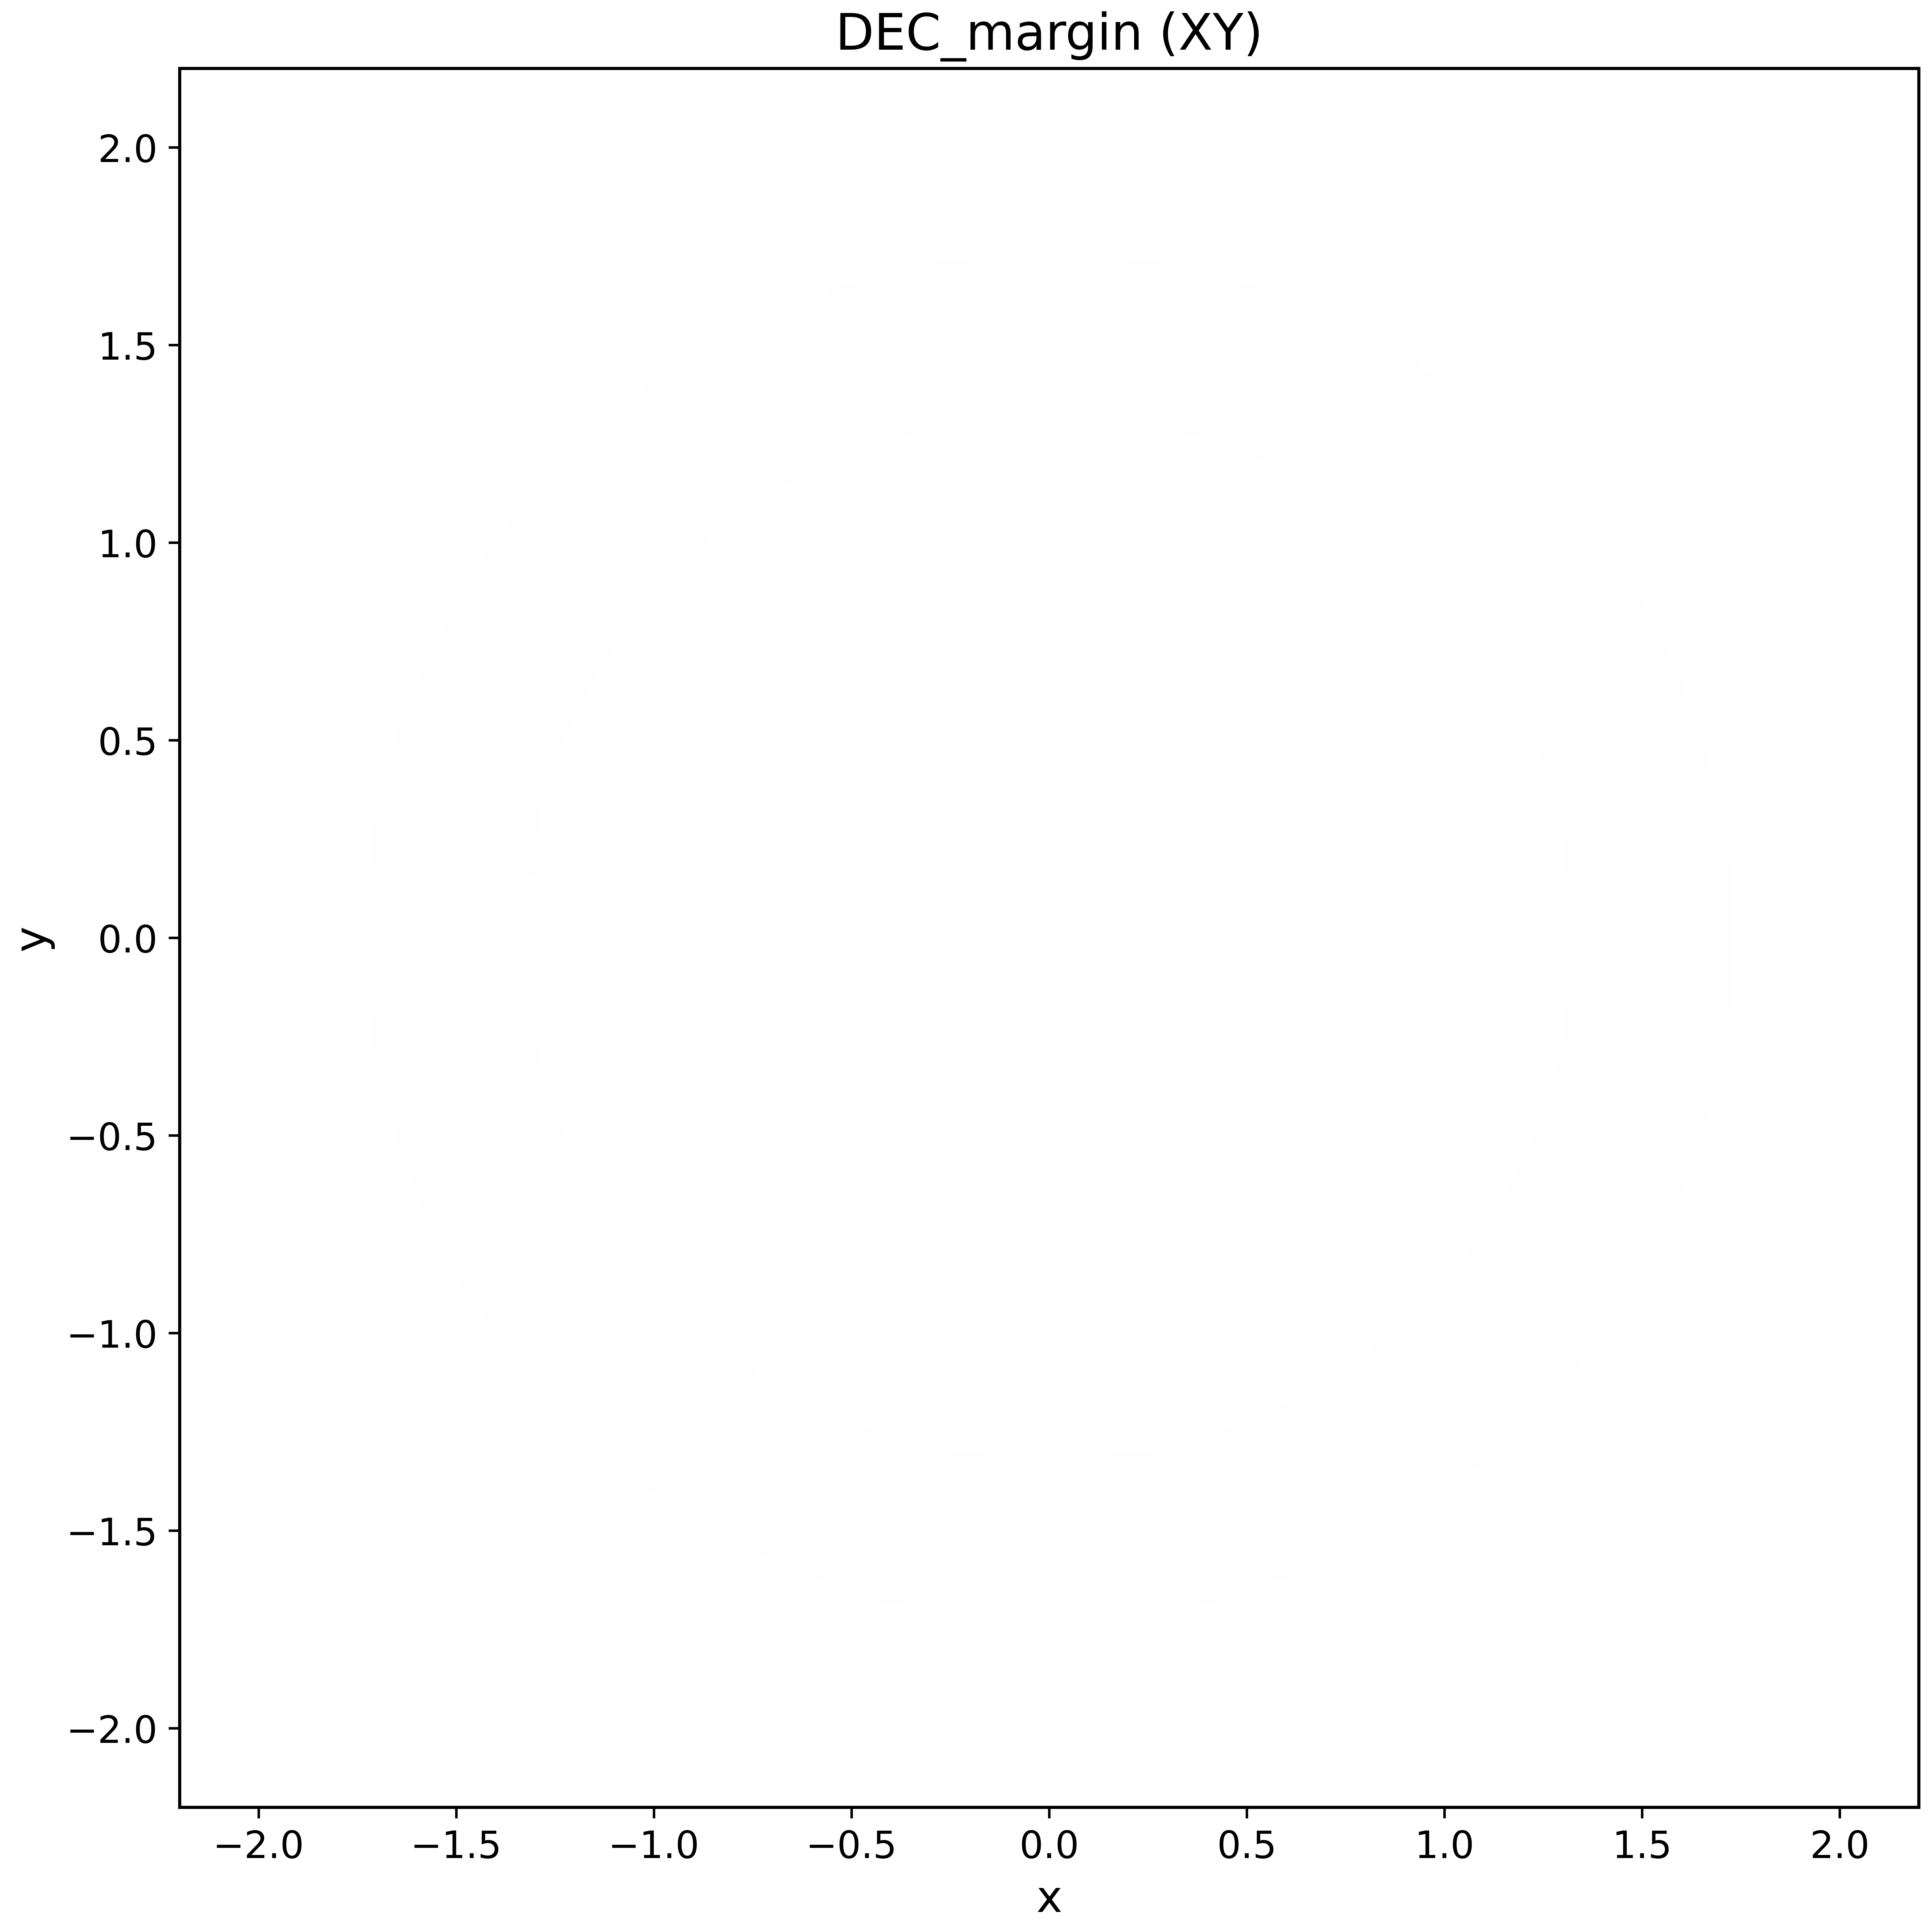
\includegraphics[width=\linewidth]{figures/domain_2_v_0p1_t_30p0_a1p848_b1p135_R01p292_XY_DECmargin.png}
    \caption{DEC margin, emphasising that the strongest violations are again tangential-stress dominated and most pronounced near the inner shell.}
    \label{fig:d2-xy-decmargin}
  \end{subfigure}\hfill
  \begin{subfigure}[b]{0.46\textwidth}
    \centering
    
\includegraphics[width=\linewidth]{figures/domain_2_v_0p1_t_30p0_a1p848_b1p135_R01p292_XY_SEC.png}
    \caption{\(\SEC\) on the equatorial slice; the trace is mixed rather than uniformly positive, but its deficits remain milder in aggregate than the corresponding DEC deficits.}
    \label{fig:d2-xy-sec}
  \end{subfigure}

  \caption{Double-shell configuration, equatorial slice:
  \DEC\ and \SEC\ diagnostics highlighting the trade-off between curvature redistribution and localized central deficits. See Table~\ref{tab:summary} and Sec.~\ref{sec:quantitative} for the corresponding quantitative summary.}
  \label{fig:d2-xy-energy-B}
\end{figure}

%-----------------------------------------------------
% Double shell: Energy conditions, XZ slice (3 panels)
%-----------------------------------------------------
\begin{figure}[htbp]
  \centering
  \begin{subfigure}[b]{0.46\textwidth}
    \centering
    
\includegraphics[width=\linewidth]{figures/domain_2_v_0p1_t_30p0_a1p848_b1p135_R01p292_XZ_rho.png}
    \caption{Energy density \(\rho\) on the meridional slice; the outer shell is clearly visible, while the inner cavity remains vacuum.}
    \label{fig:d2-xz-rho}
  \end{subfigure}\hfill
  \begin{subfigure}[b]{0.46\textwidth}
    \centering
    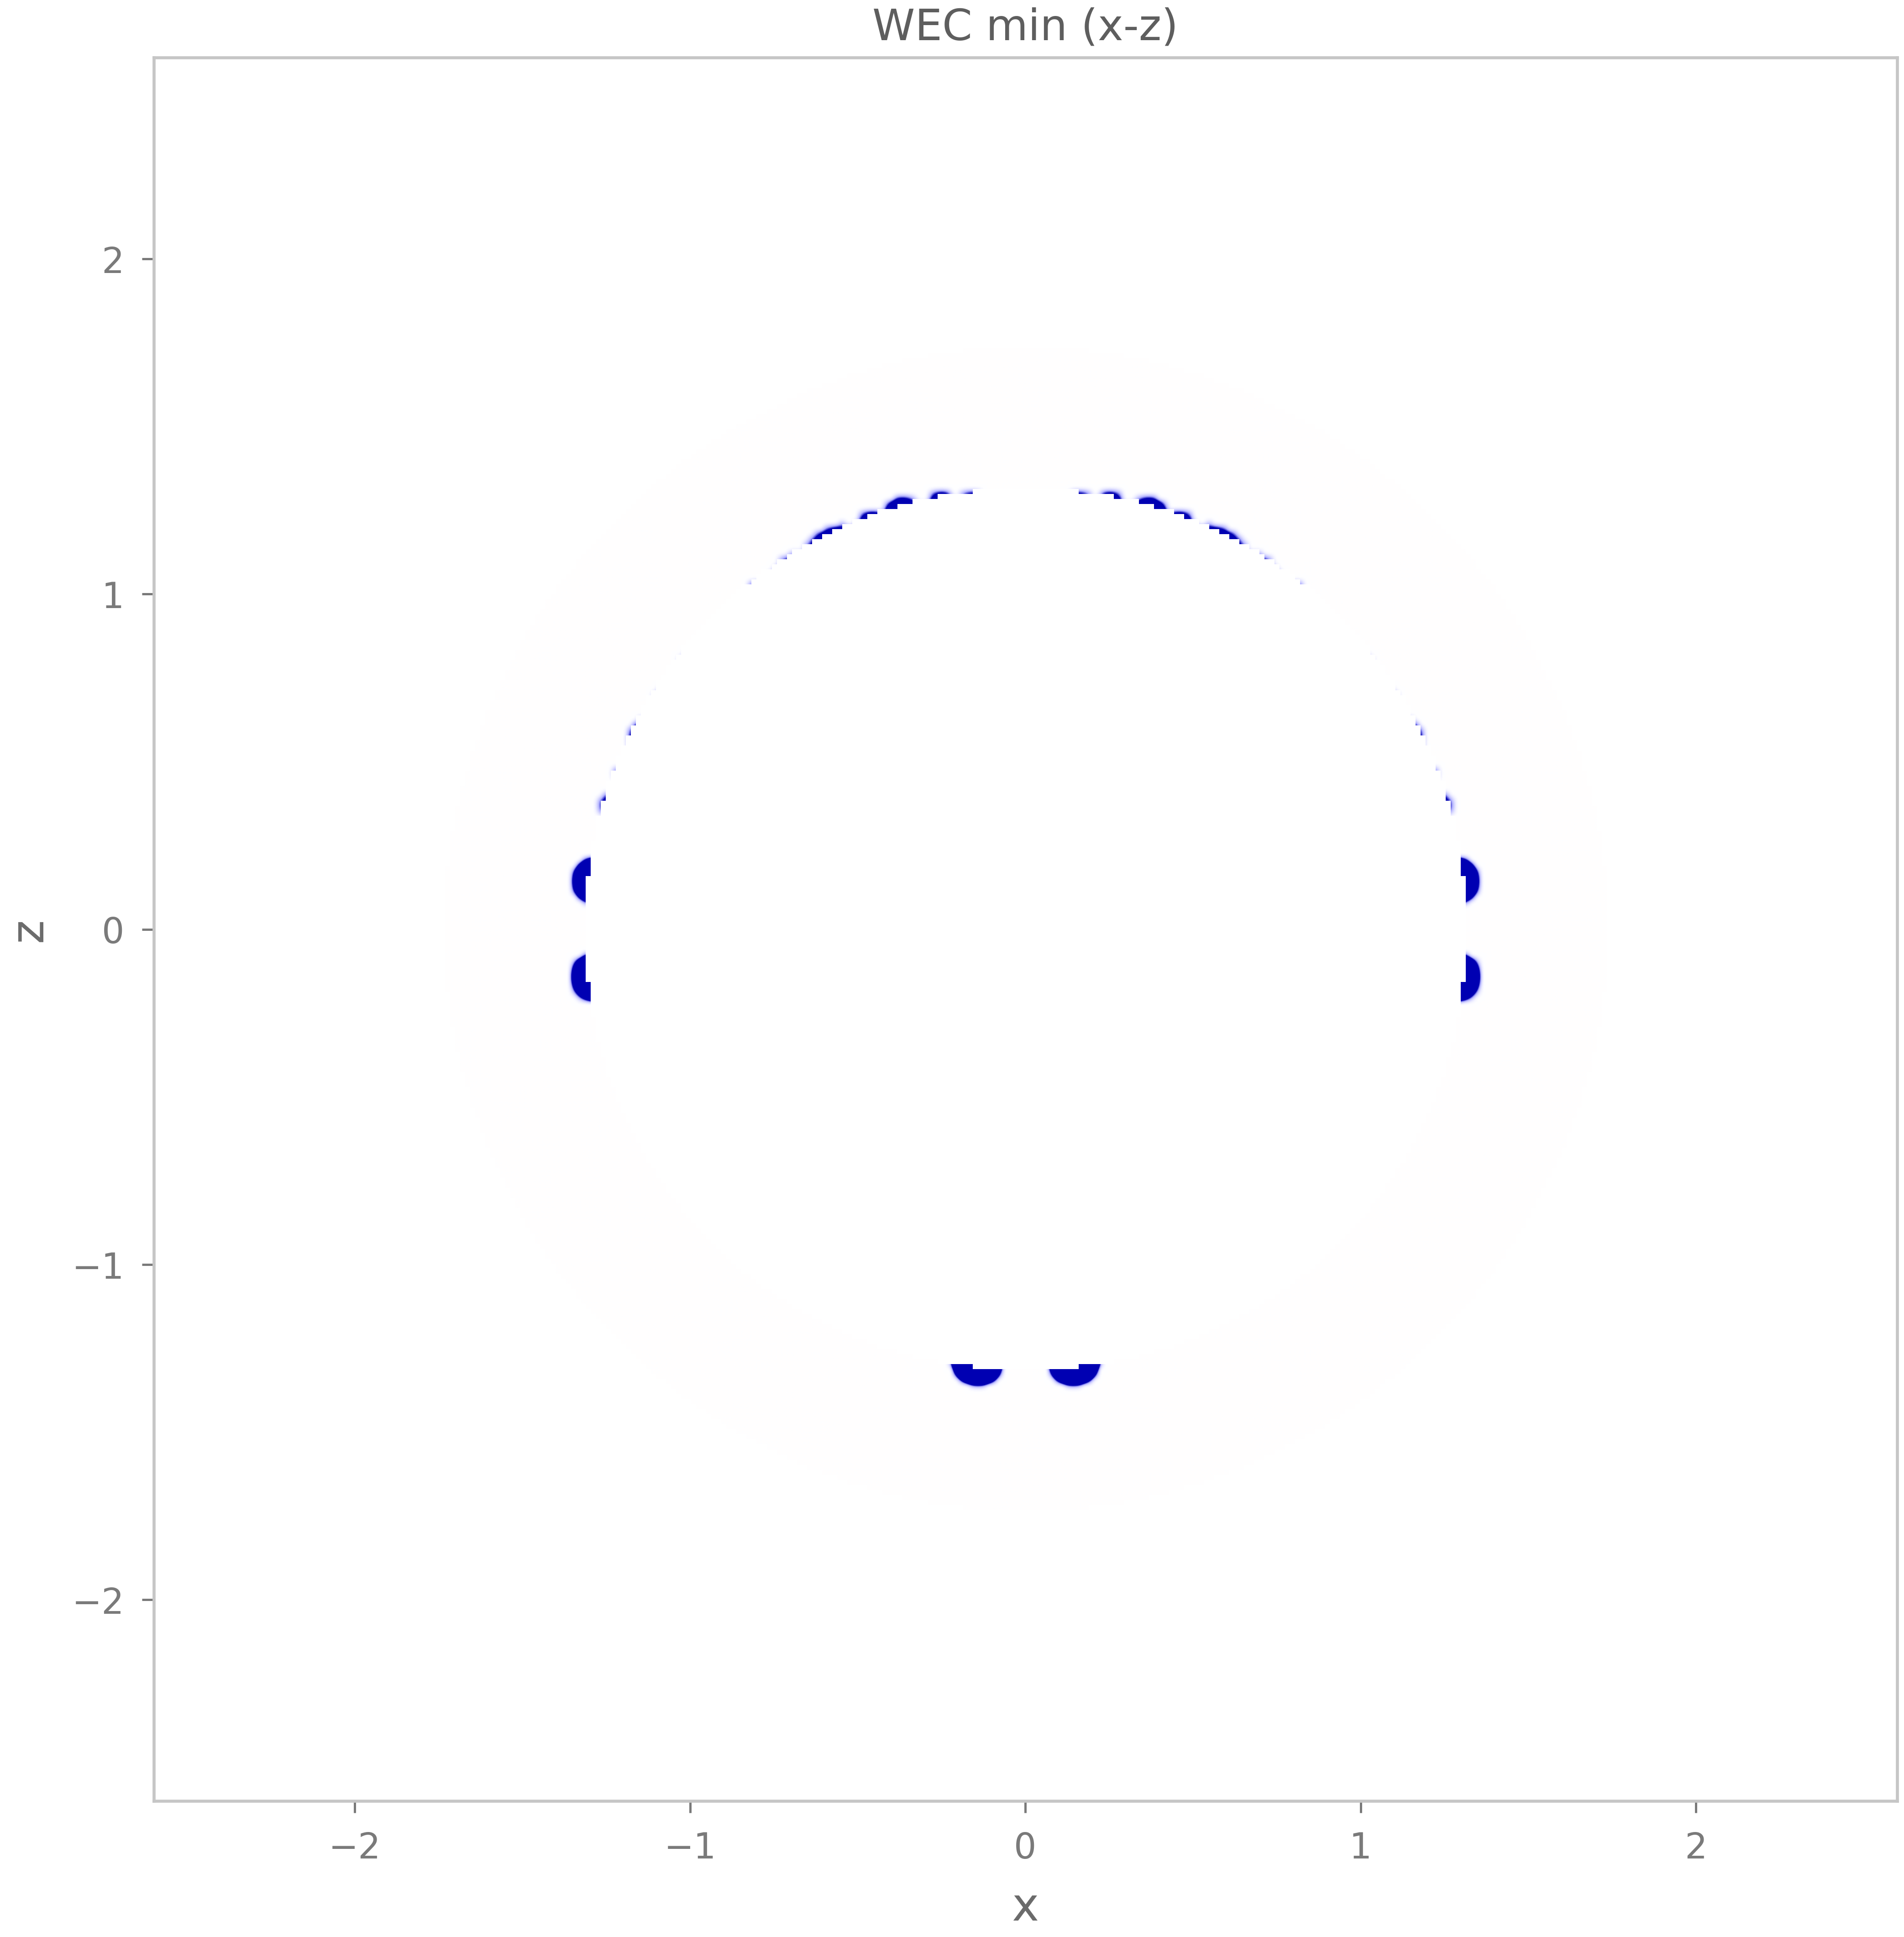
\includegraphics[width=\linewidth]{figures/domain_2_v_0p1_t_30p0_a1p848_b1p135_R01p292_XZ_WECmin.png}
    \caption{\(\mathrm{WEC}_{\min}\) along \(x\mbox{--}z\); violations are localized near the inner interface and slightly elongated along the direction of motion.}
    \label{fig:d2-xz-wecmin}
  \end{subfigure}

  \vspace{1ex}

  \begin{subfigure}[b]{0.46\textwidth}
    \centering
    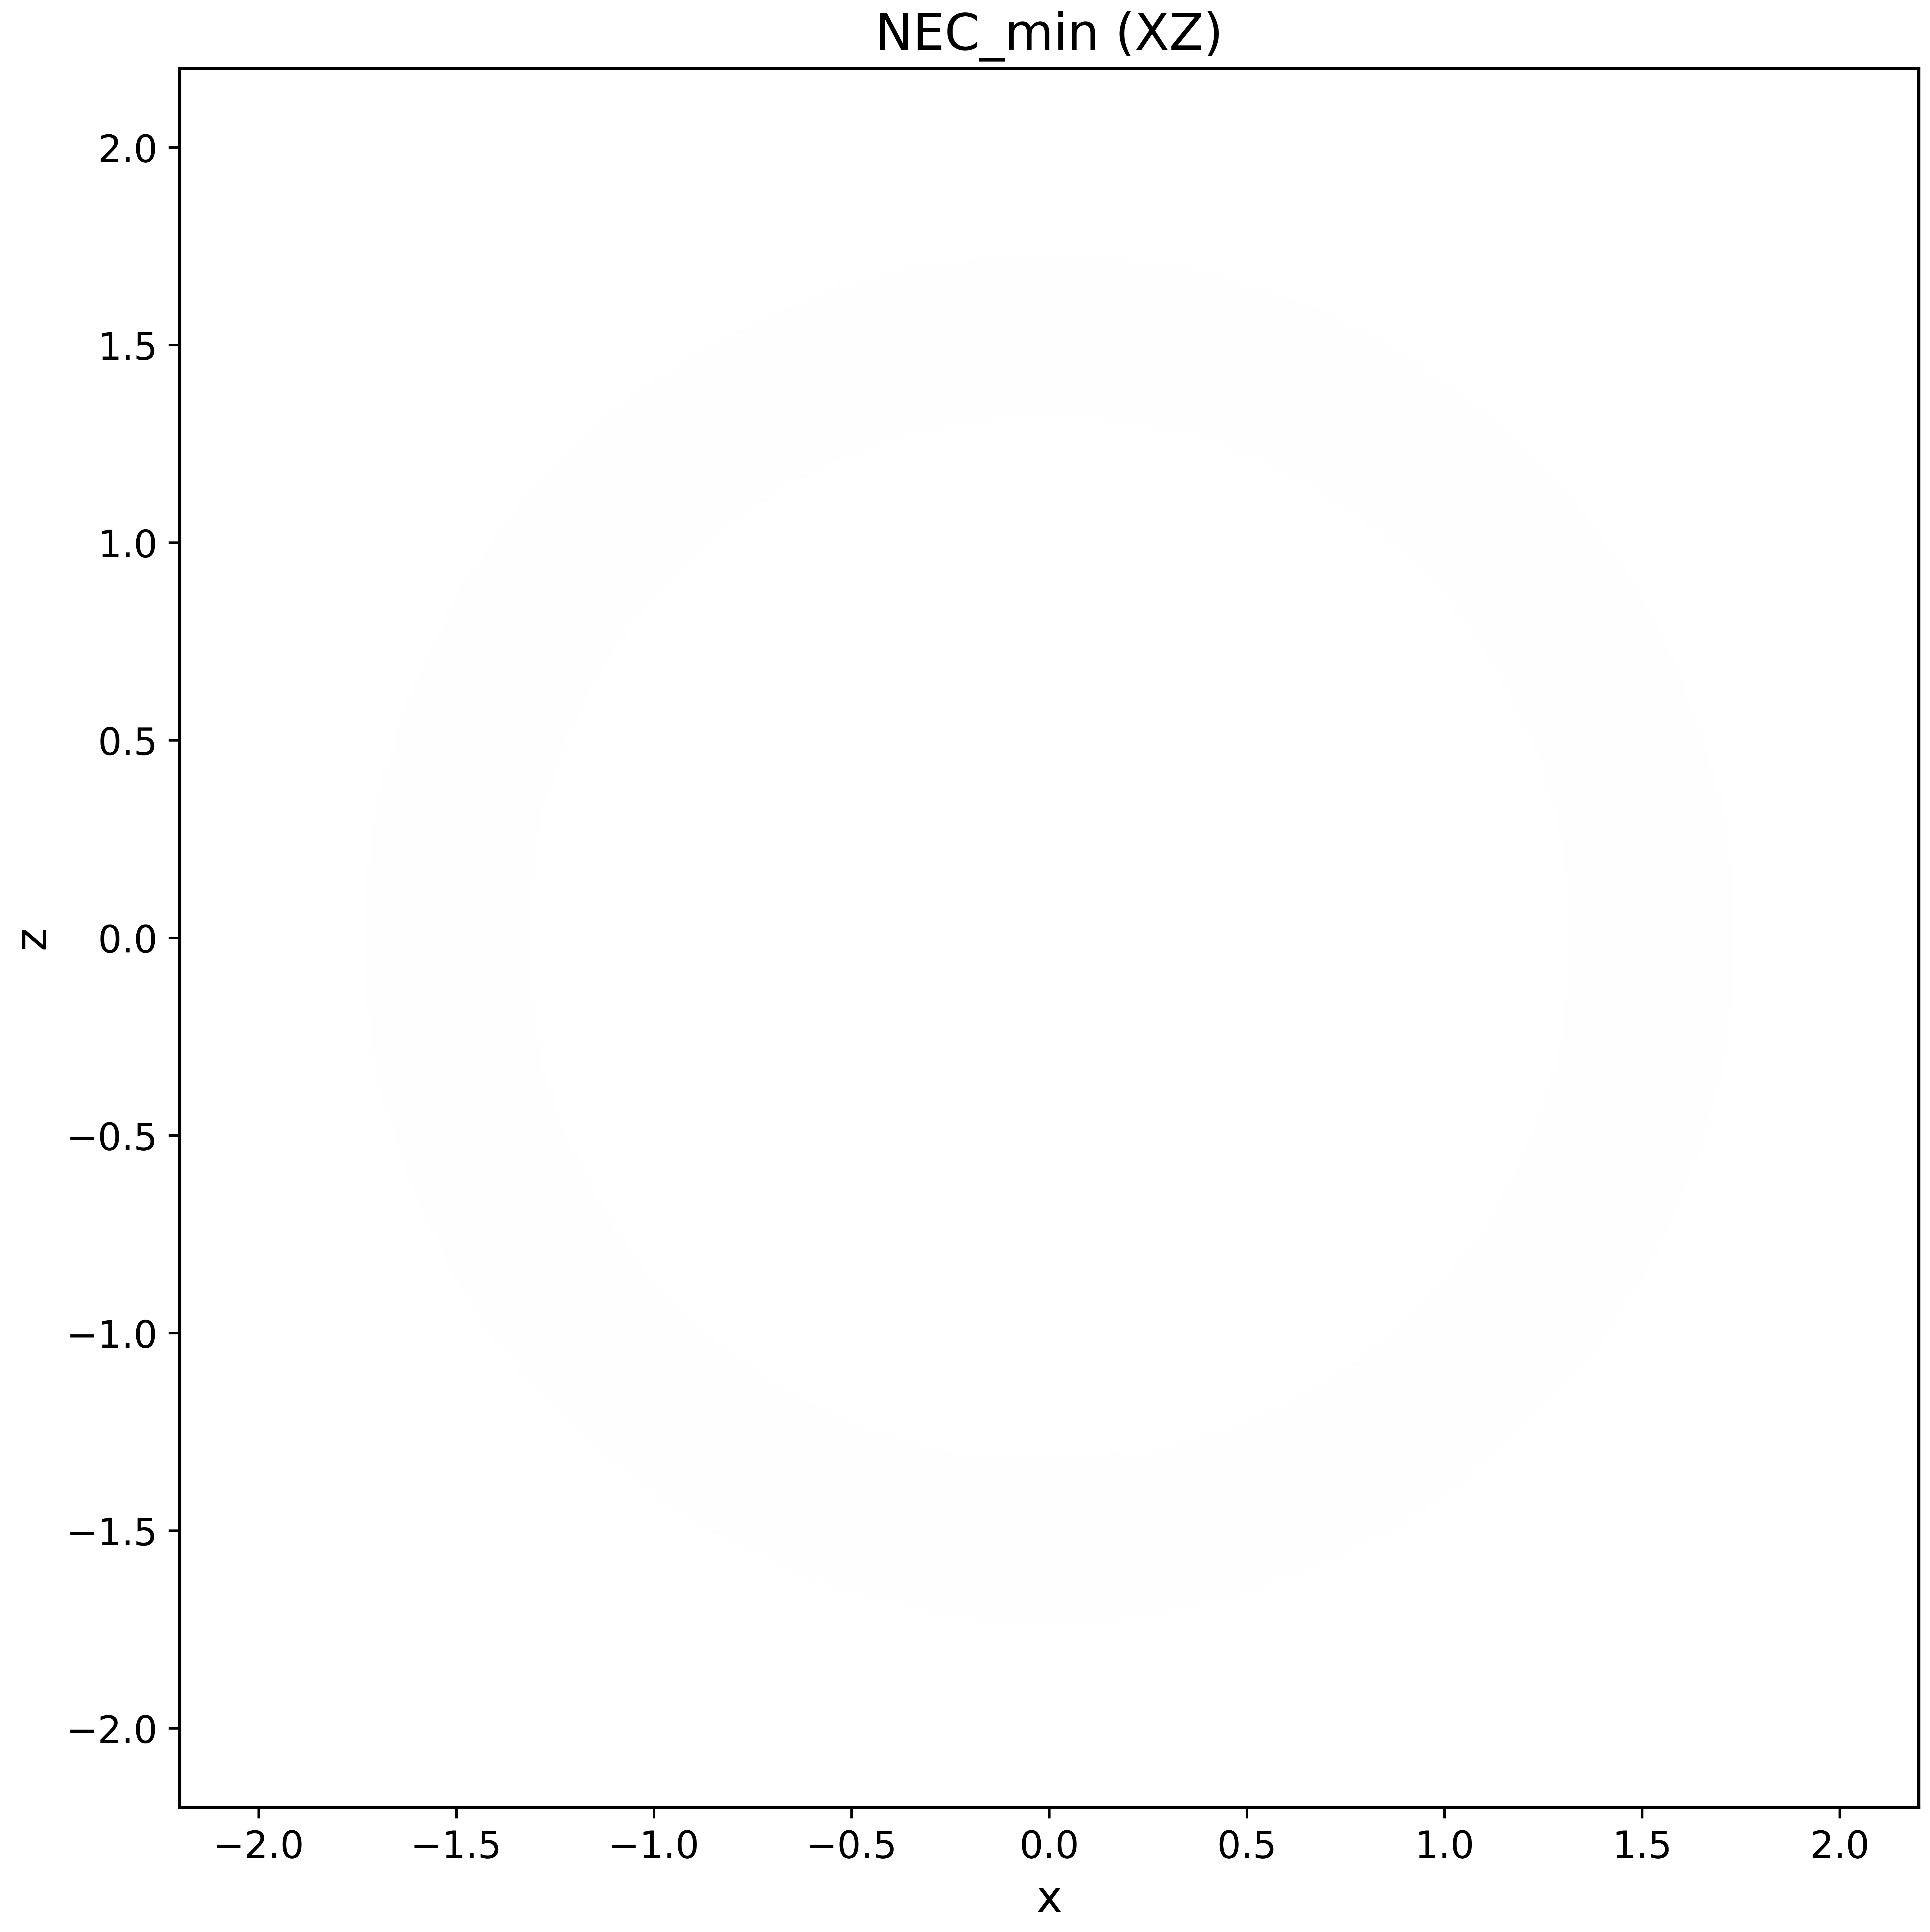
\includegraphics[width=\linewidth]{figures/domain_2_v_0p1_t_30p0_a1p848_b1p135_R01p292_XZ_NECmin.png}
    \caption{\(\mathrm{NEC}_{\min}\) with the same morphology, confirming that the central deficits seen in Fig.~\ref{fig:d2-xy-energy-A} are genuinely three-dimensional.}
    \label{fig:d2-xz-necmin}
  \end{subfigure}

  \caption{Double-shell configuration, meridional \(x\mbox{--}z\) slice:
  density and minimum \WEC/\NEC\ margins, providing the complementary view to Fig.~\ref{fig:d2-xy-energy-A}.}
  \label{fig:d2-xz-energy-A}
\end{figure}

%-----------------------------------------------------
% Double shell: Energy conditions, XZ slice (2 panels)
%-----------------------------------------------------
\begin{figure}[htbp]
  \centering
  \begin{subfigure}[b]{0.46\textwidth}
    \centering
    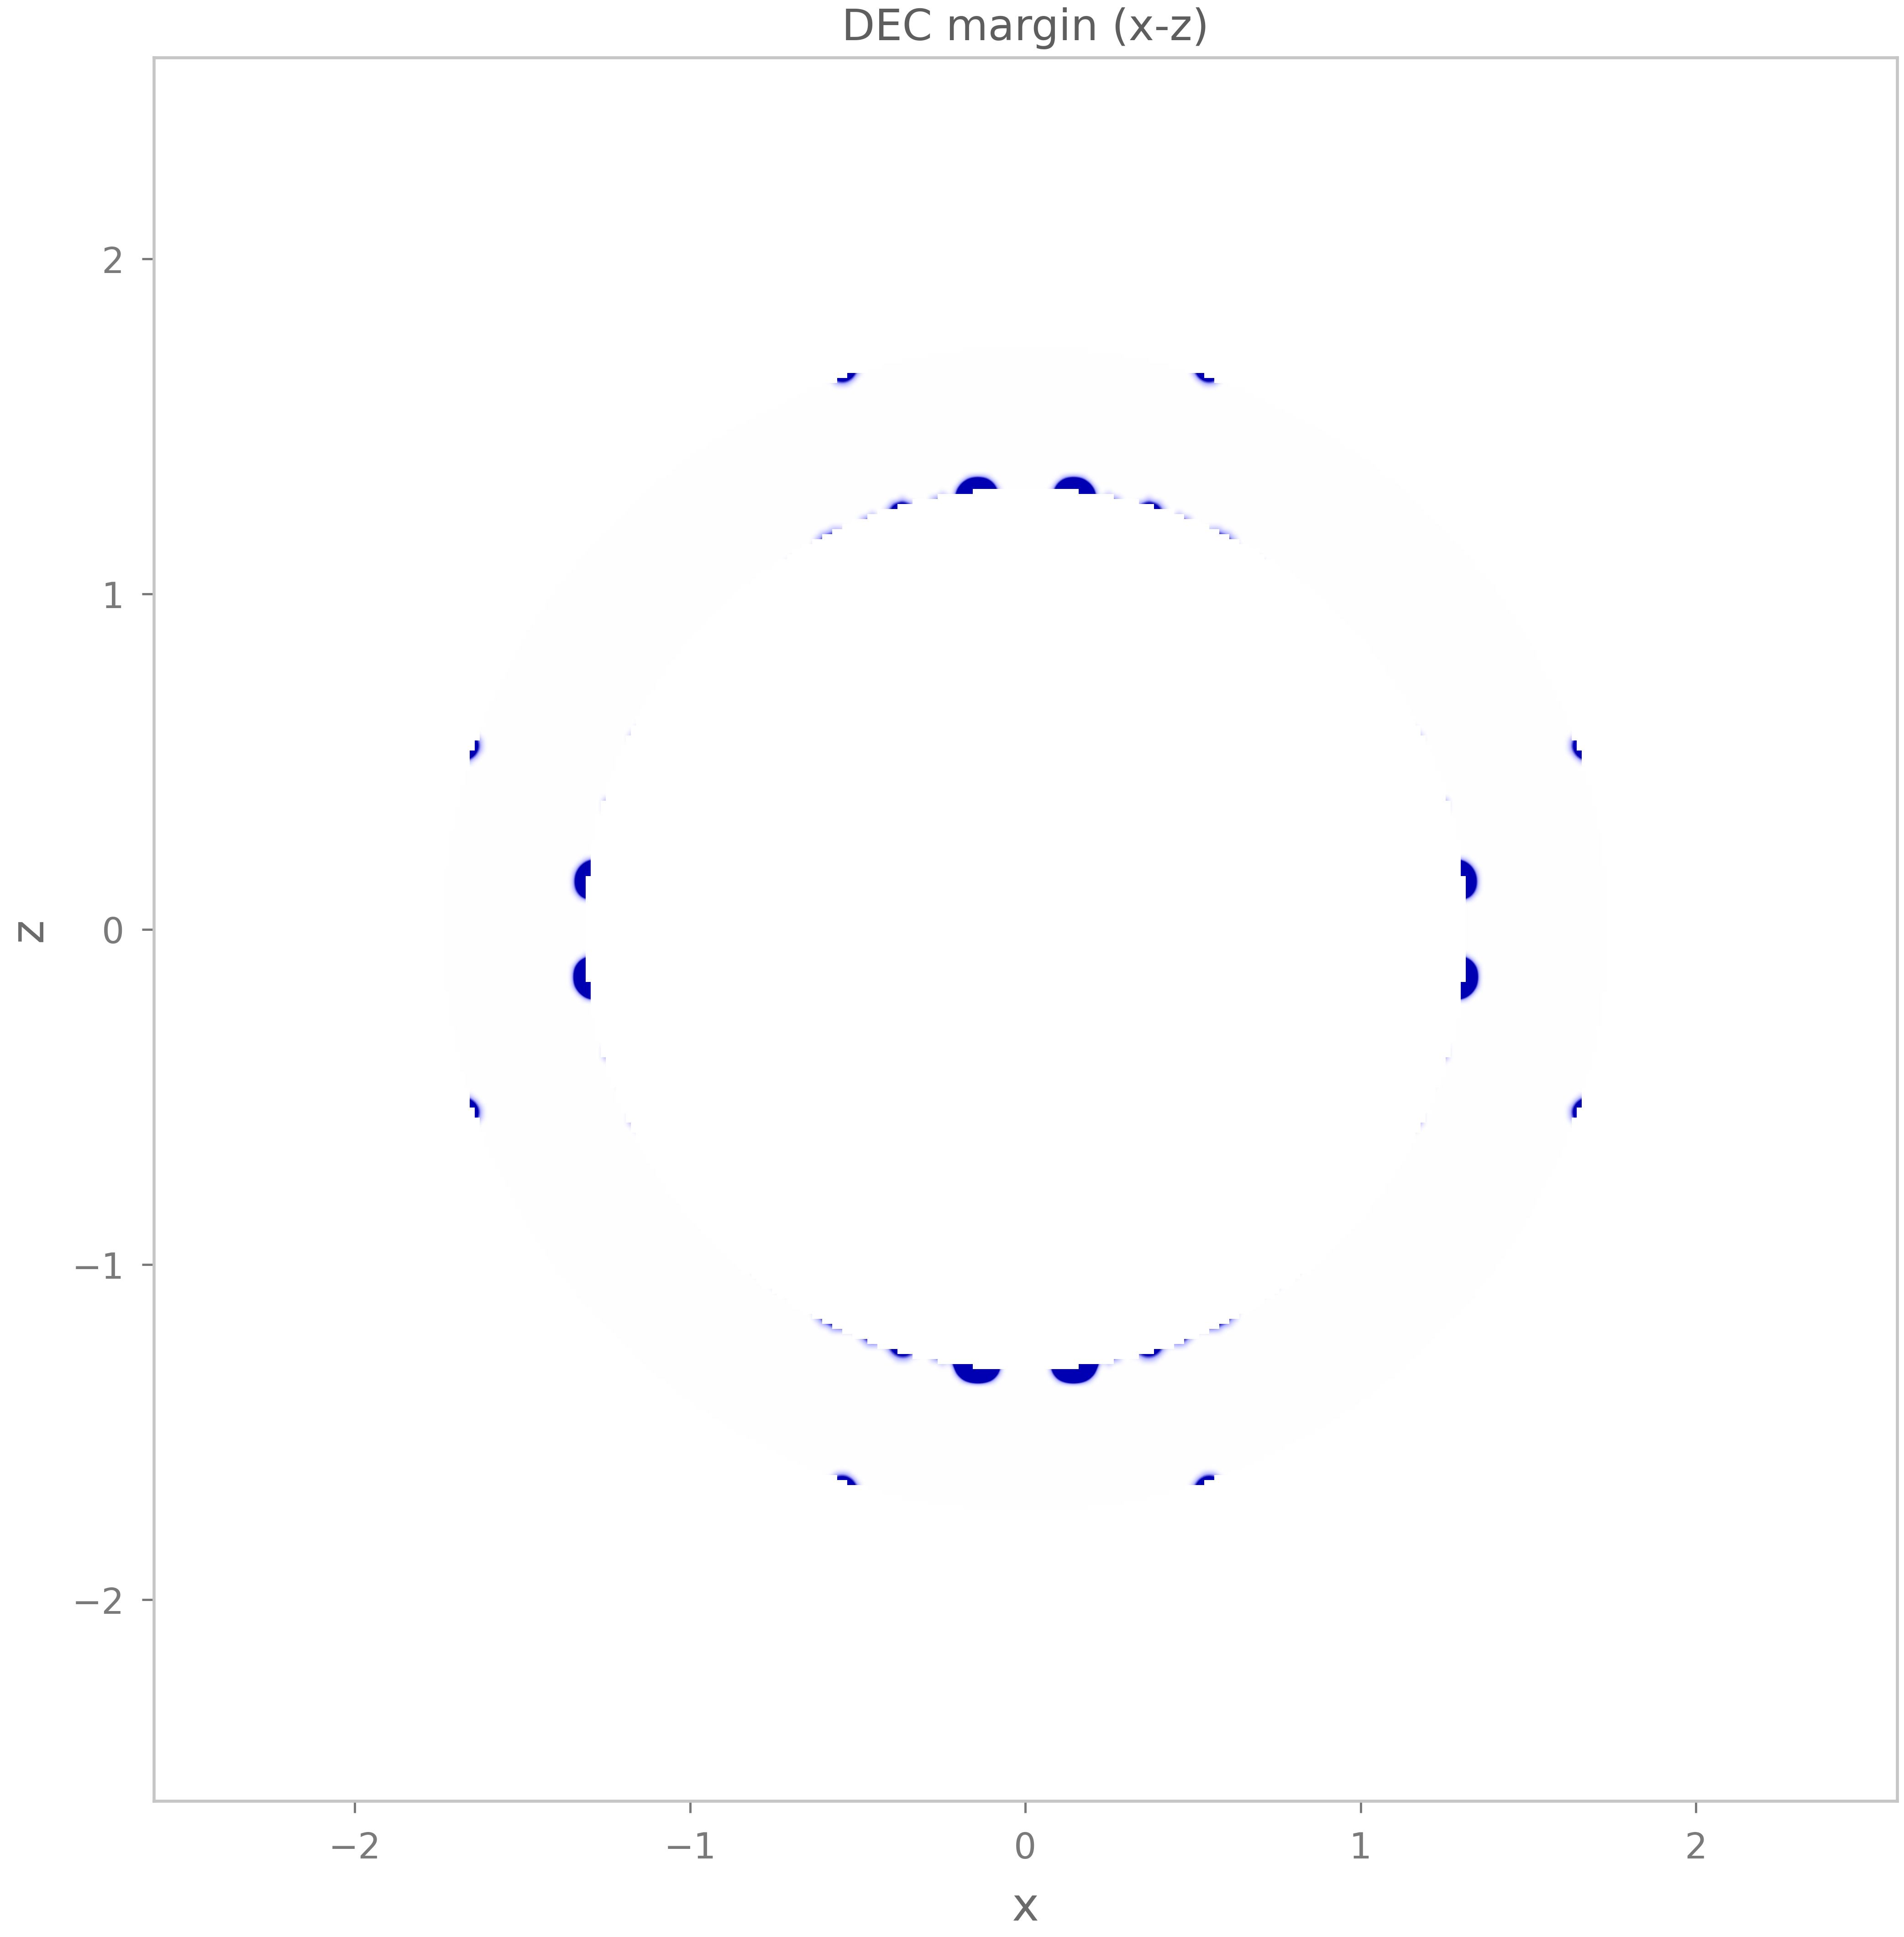
\includegraphics[width=\linewidth]{figures/domain_2_v_0p1_t_30p0_a1p848_b1p135_R01p292_XZ_DECmargin.png}
    \caption{DEC margin on the meridional slice, showing how tangential-stress excess spreads slightly along the equatorial plane but remains tied to the interfaces.}
    \label{fig:d2-xz-decmargin}
  \end{subfigure}\hfill
  \begin{subfigure}[b]{0.46\textwidth}
    \centering
    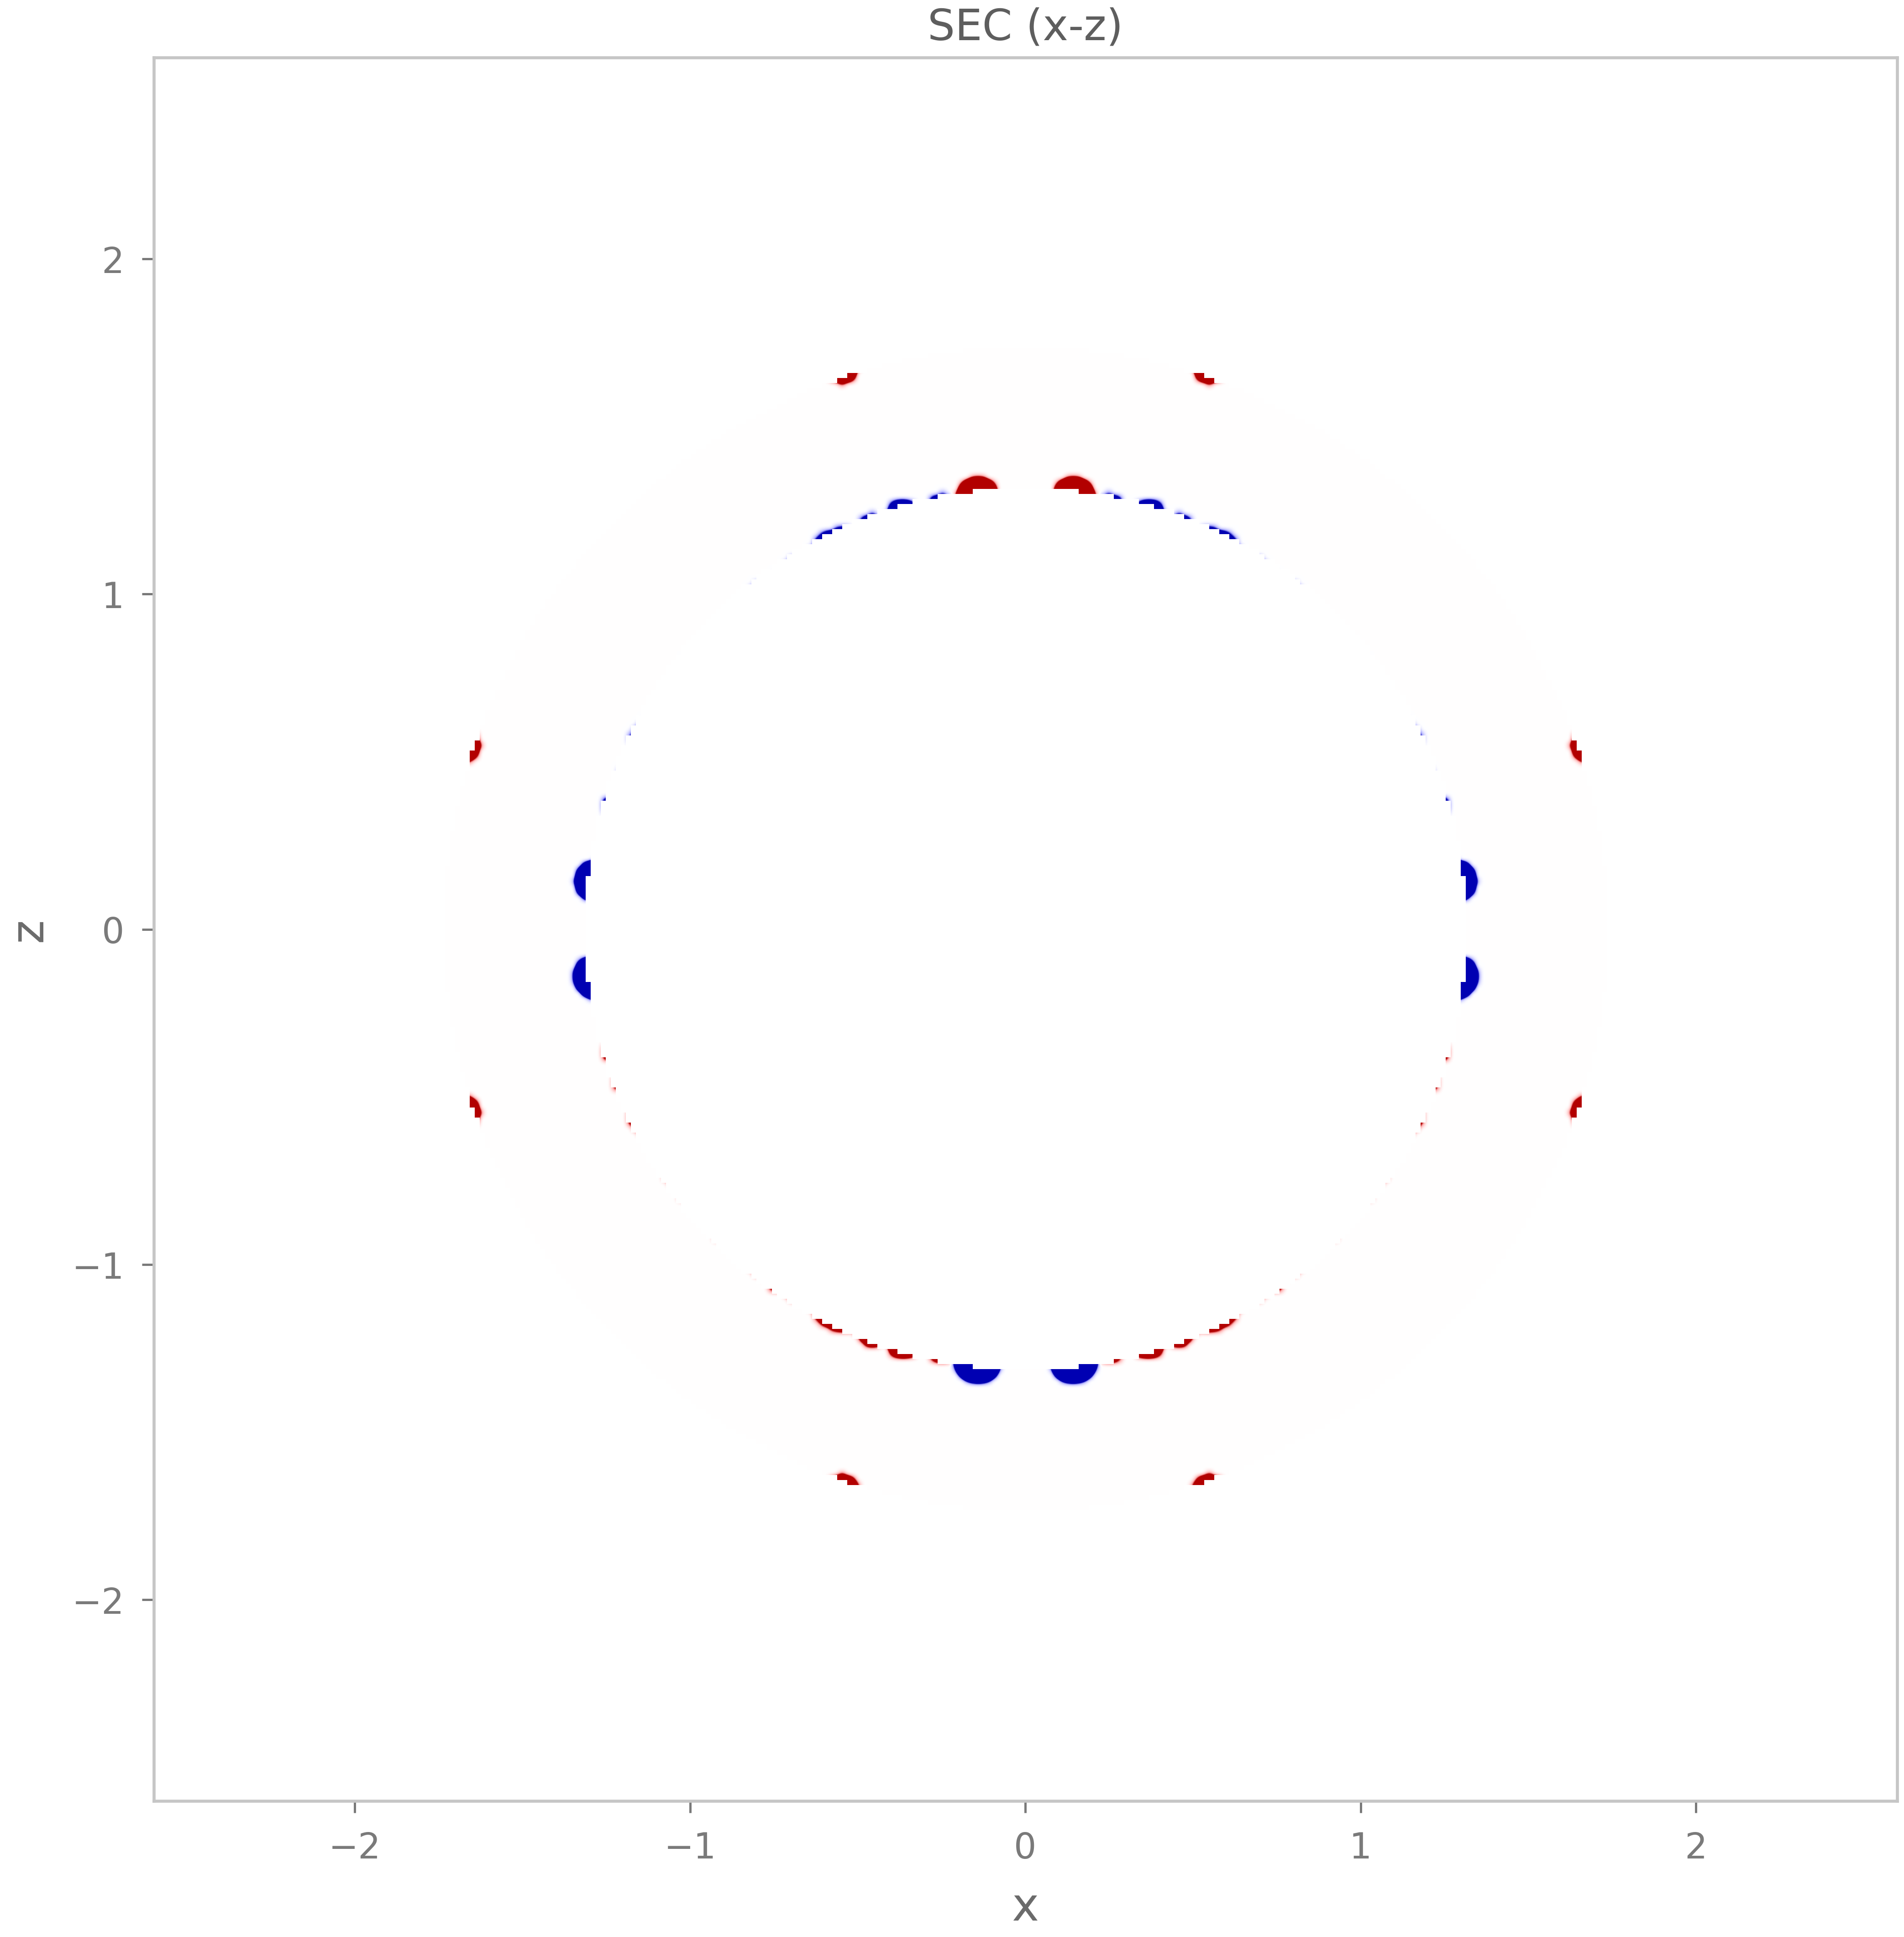
\includegraphics[width=\linewidth]{figures/domain_2_v_0p1_t_30p0_a1p848_b1p135_R01p292_XZ_SEC.png}
    \caption{\(\SEC\) on the same slice; the pattern is sign-changing but remains less restrictive in aggregate than the \DEC, consistent with the higher final SEC success fraction.}
    \label{fig:d2-xz-sec}
  \end{subfigure}

  \caption{Double-shell configuration, meridional slice:
  \DEC\ and \SEC\ diagnostics, completing the three-dimensional picture of stress localization.}
  \label{fig:d2-xz-energy-B}
\end{figure}

%-----------------------------------------------------
% Single shell: Optimization diagnostics
%-----------------------------------------------------
\begin{figure}[p]
  \centering

  \begin{subfigure}[t]{0.47\textwidth}
    \centering
    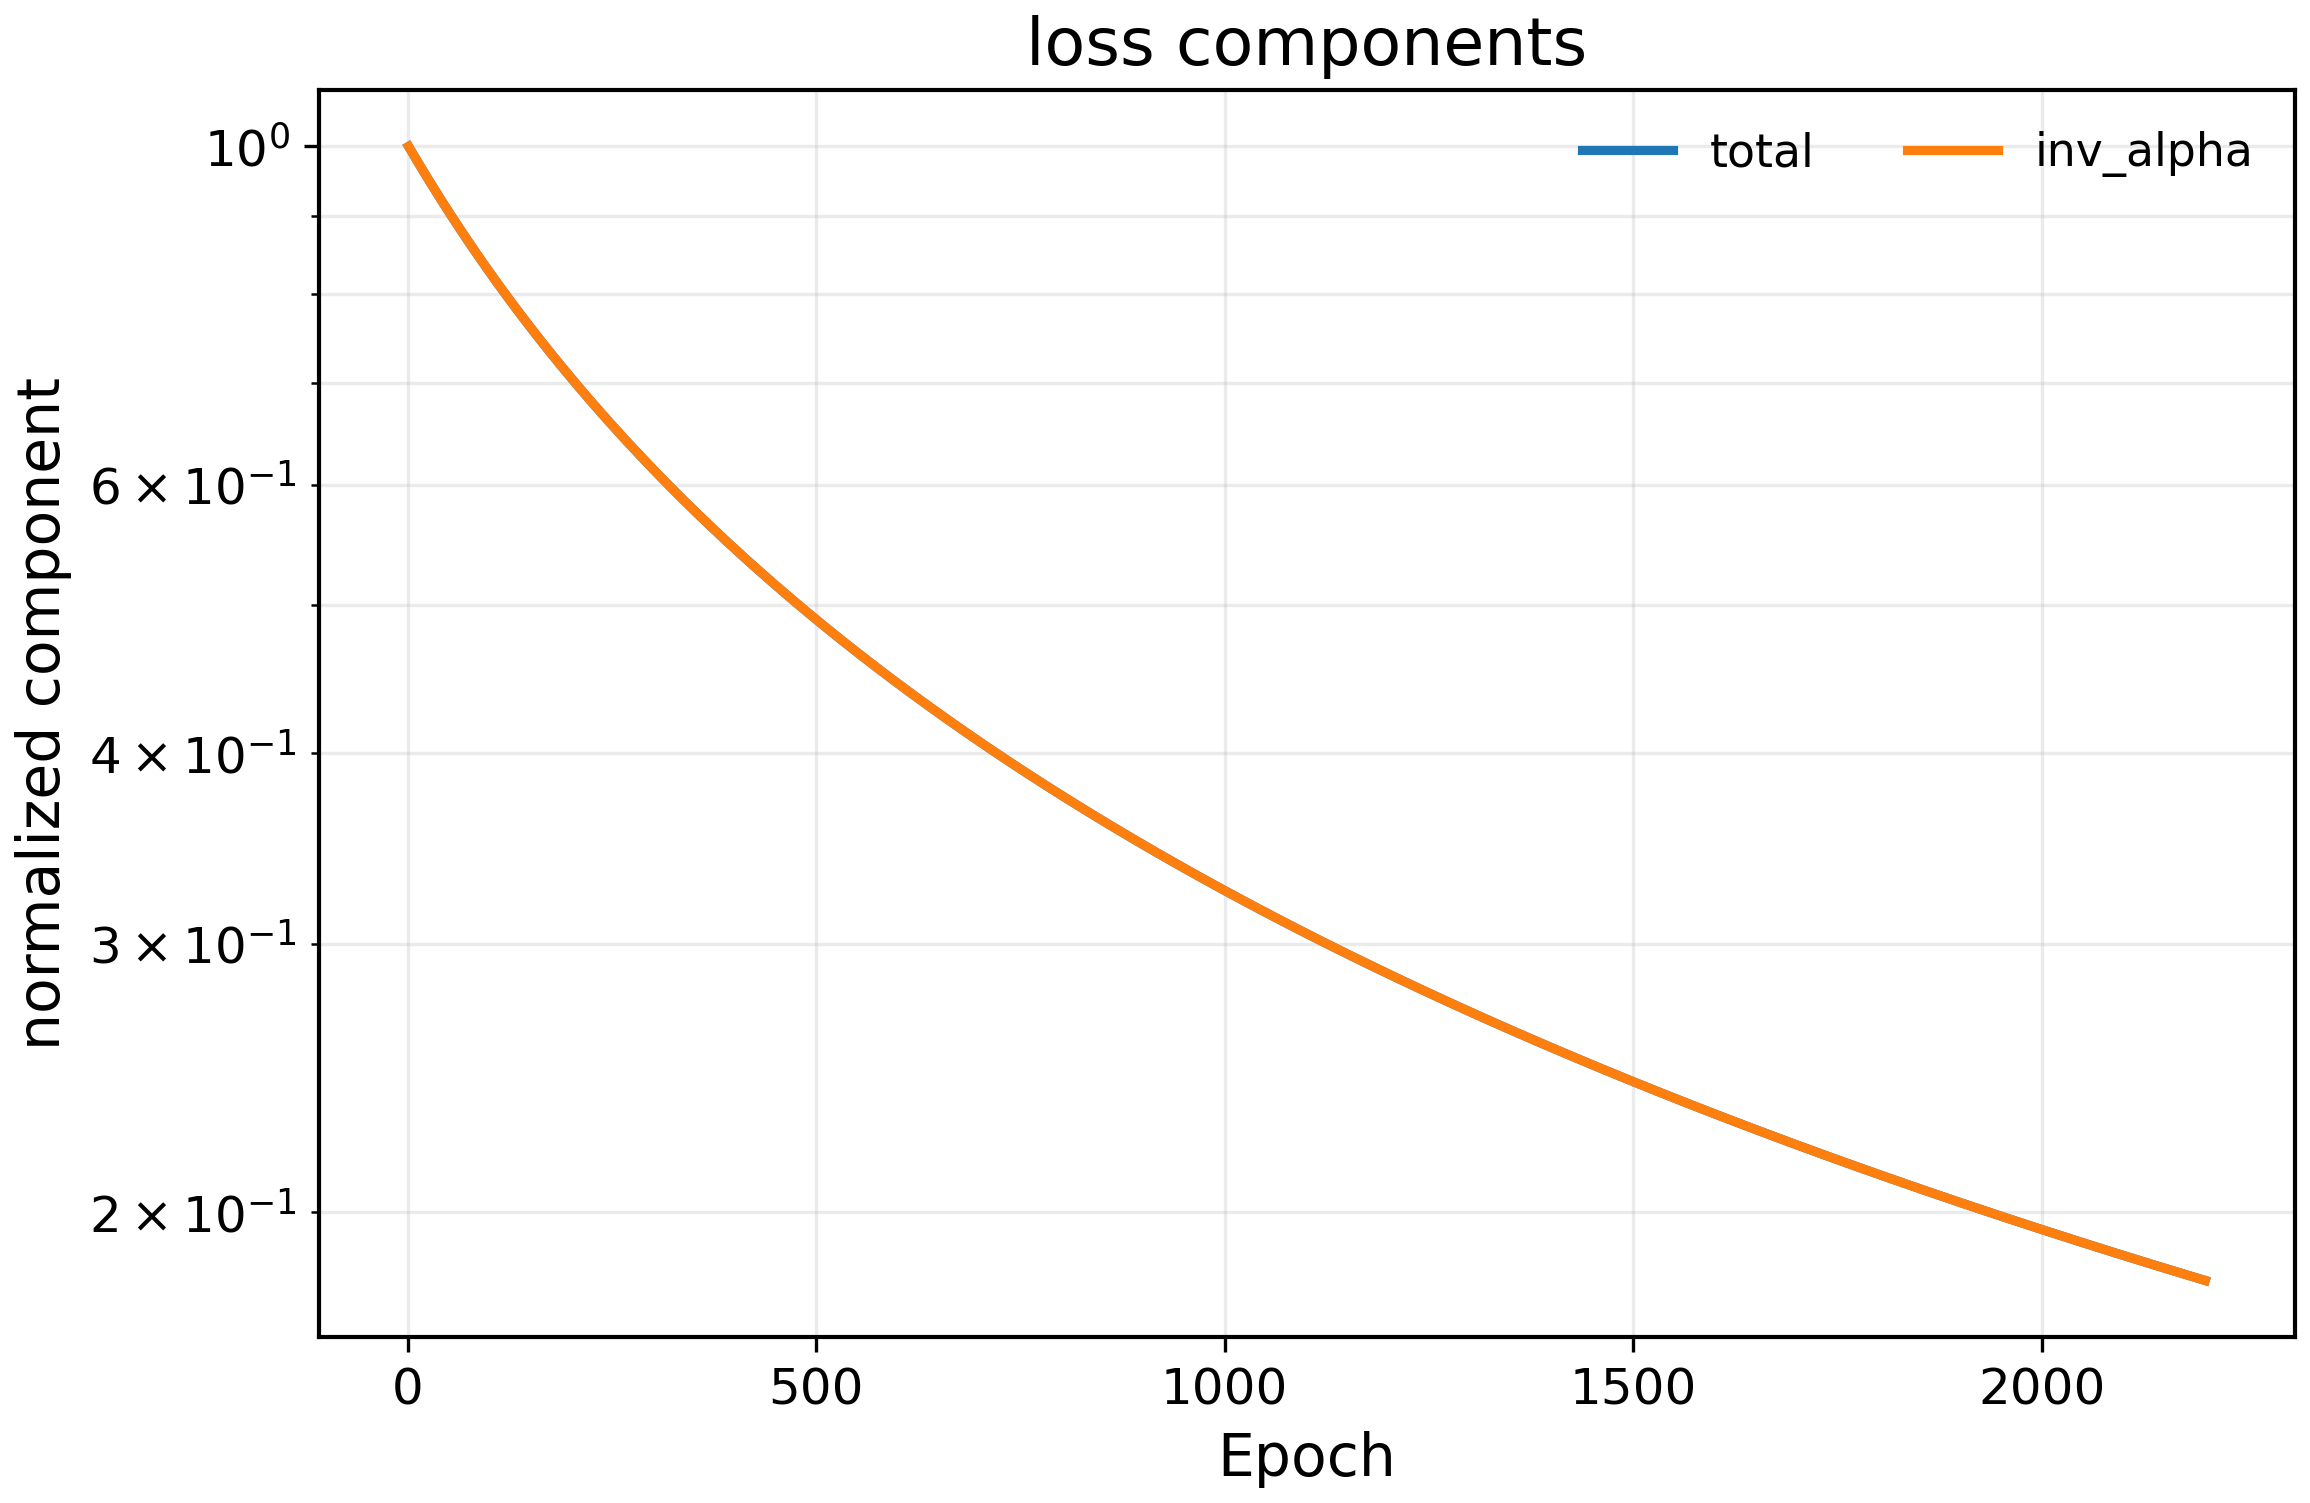
\includegraphics[width=\linewidth]{figures/domain_1_v_0p1_t_30p0_loss_components.png}
    \caption{Loss components across epochs.}
    \label{fig:d1-loss-components}
  \end{subfigure}\hfill
  \begin{subfigure}[t]{0.47\textwidth}
    \centering
    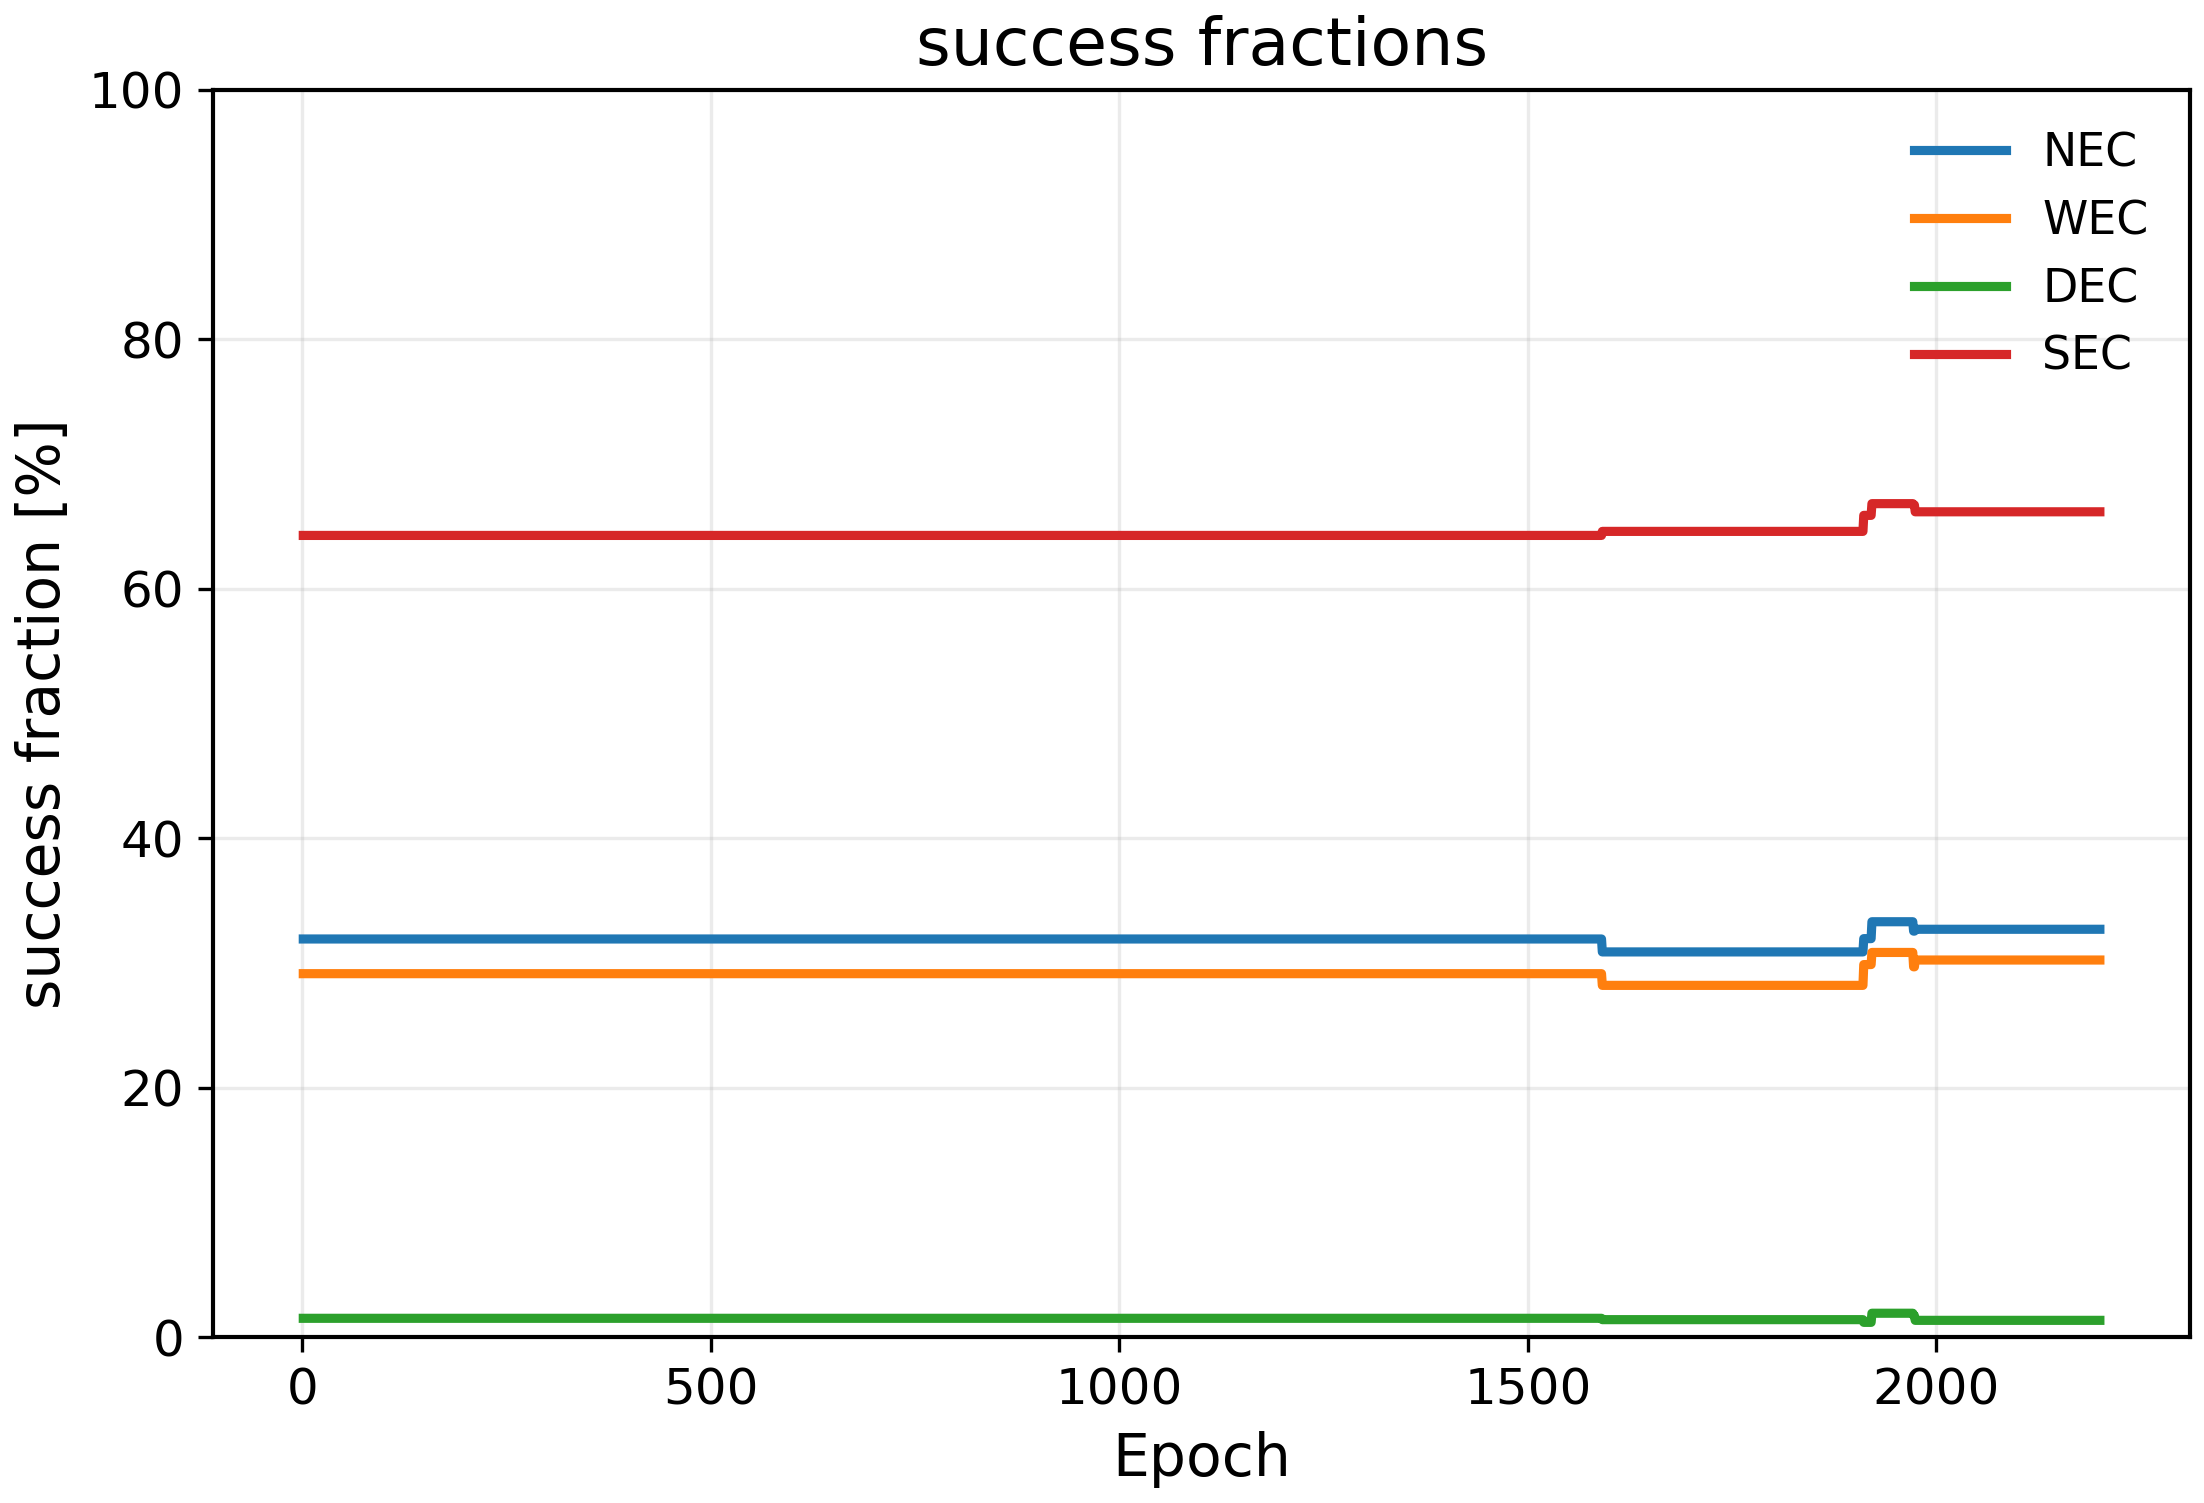
\includegraphics[width=\linewidth]{figures/domain_1_v_0p1_t_30p0_success_fractions.png}
    \caption{Success fractions for NEC/WEC/DEC/SEC.}
    \label{fig:d1-success}
  \end{subfigure}

  \vspace{1ex}

  \begin{subfigure}[t]{0.62\textwidth}
    \centering
    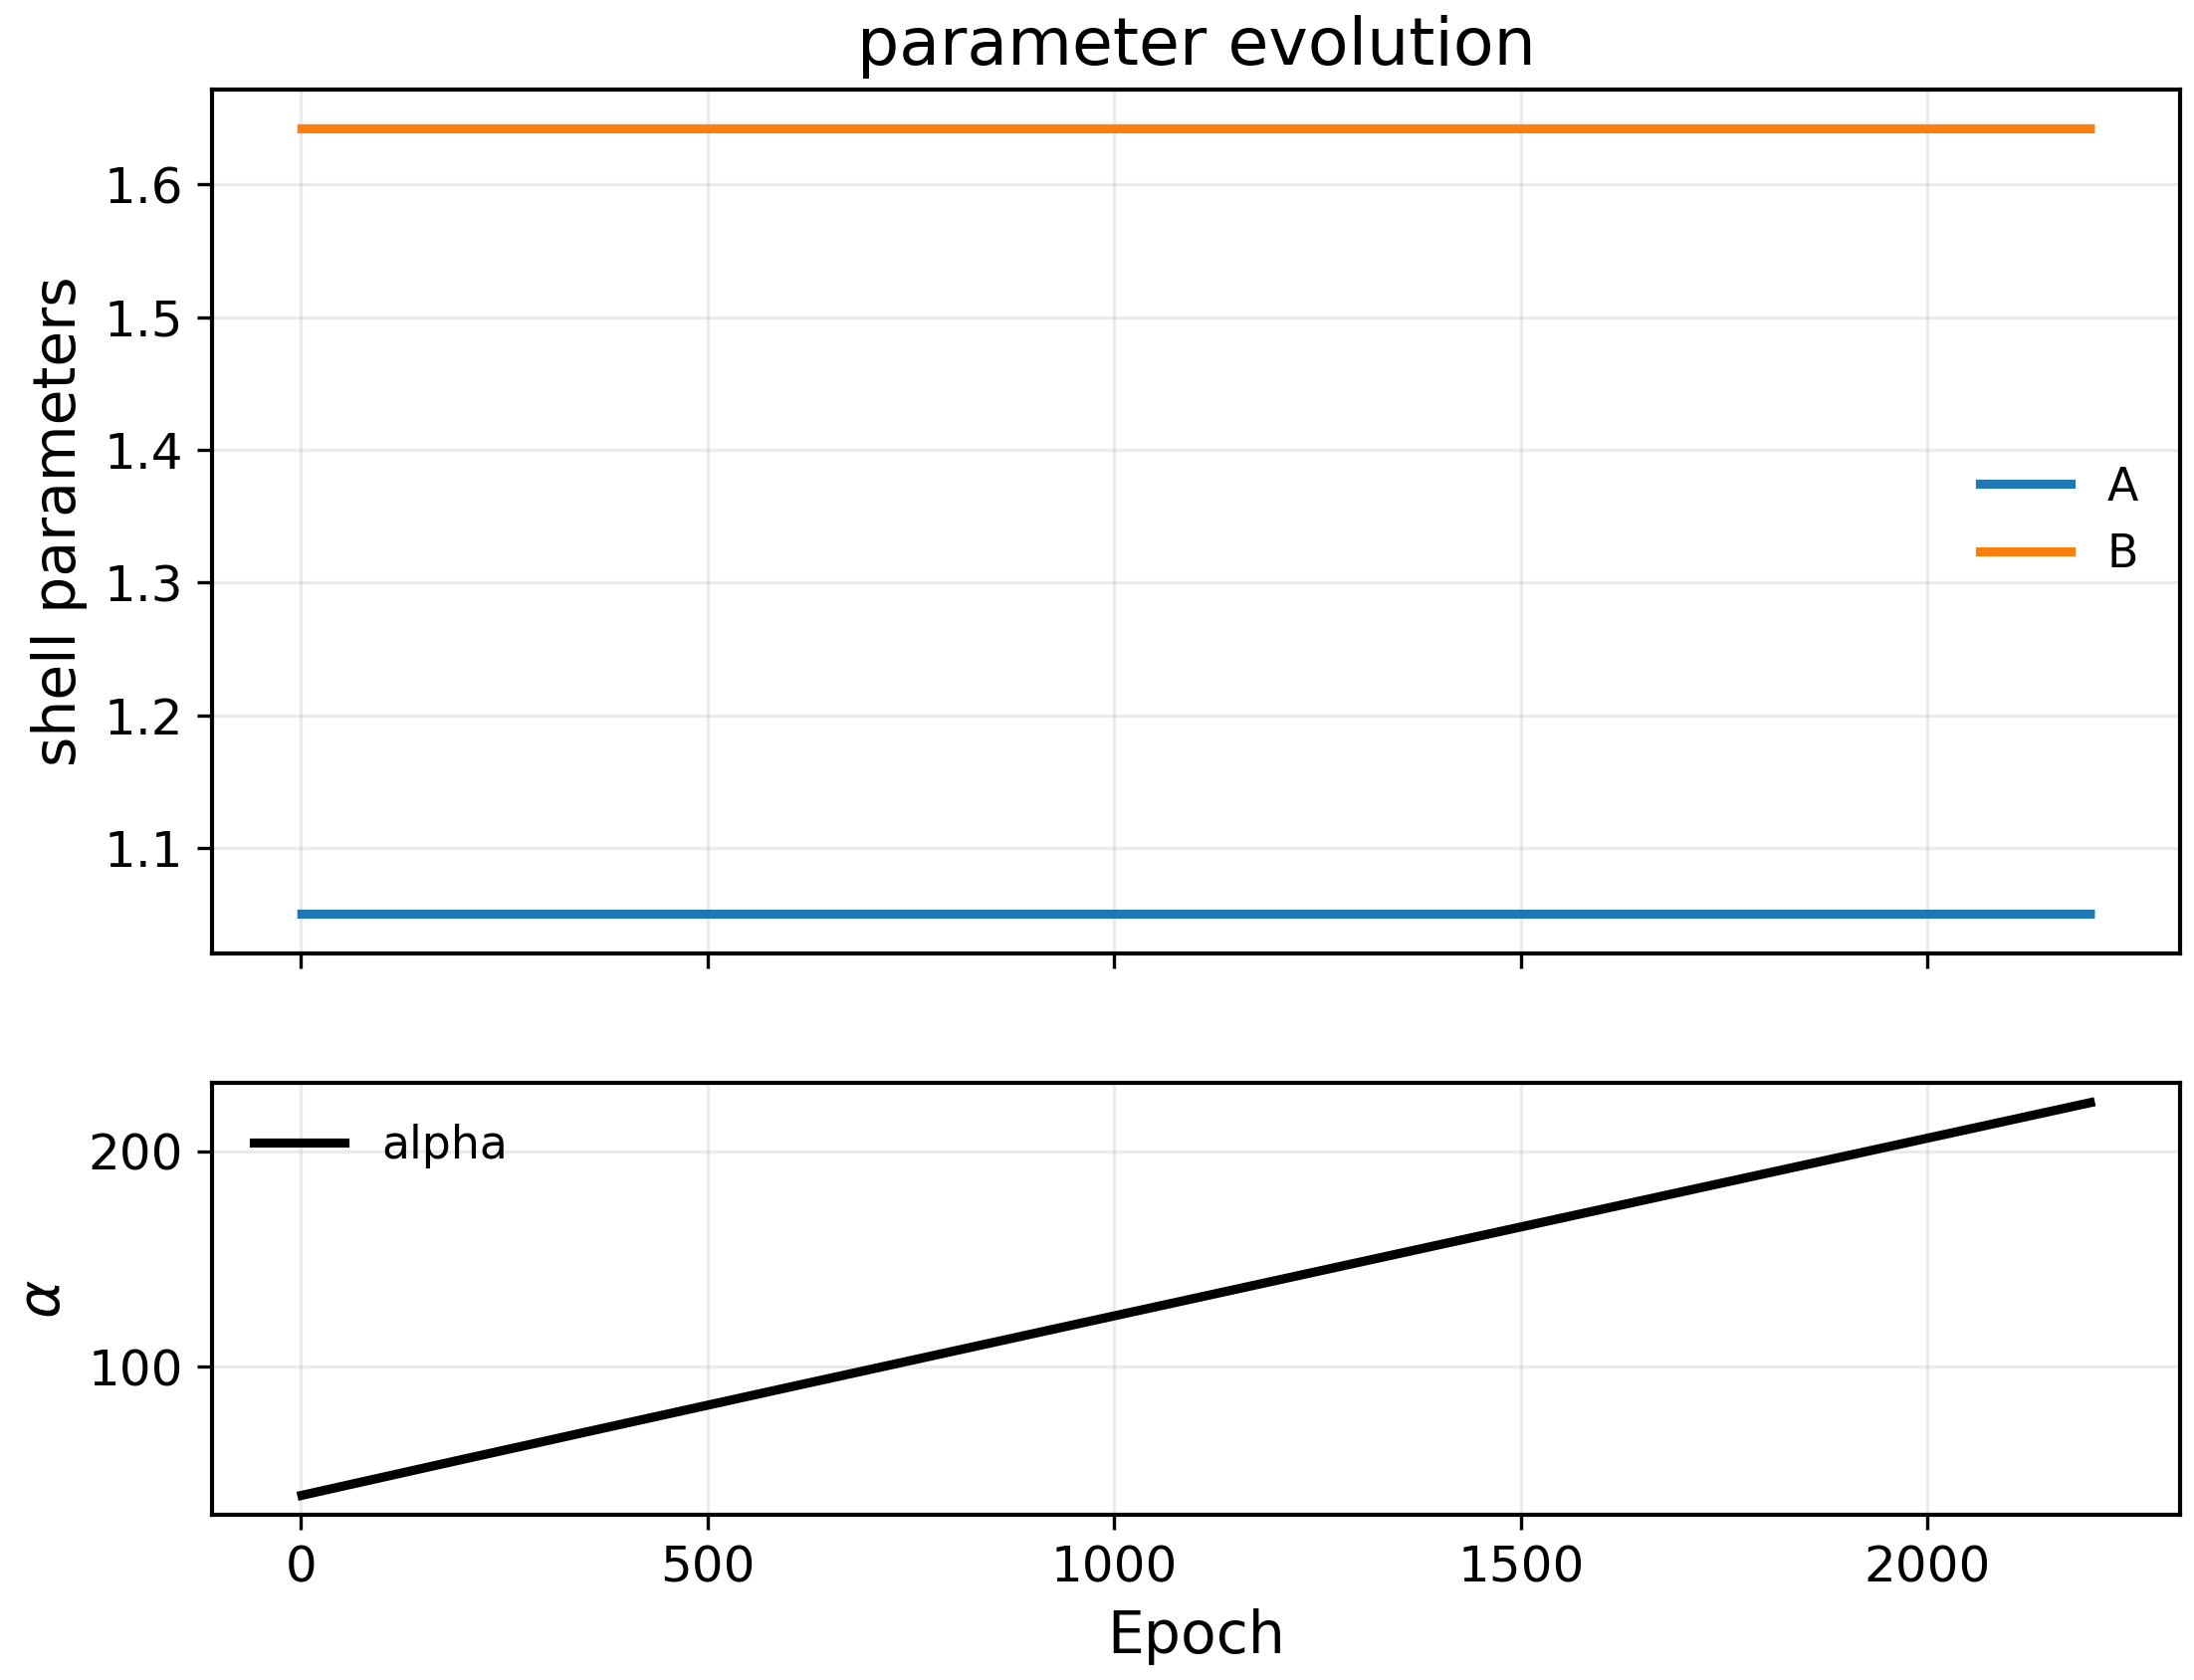
\includegraphics[width=\linewidth]{figures/domain_1_v_0p1_t_30p0_params.png}
    \caption{Seed parameters $A$ and $B$ across epochs.}
    \label{fig:d1-params-epoch}
  \end{subfigure}

  \caption{Optimization diagnostics for the single-shell configuration at $v=0.1$, $t=30$. Panel (a) shows the normalized loss terms \texttt{inv\_alpha}, \texttt{physics\_loss}, \texttt{reg\_breach}, and \texttt{total\_loss}. Panel (b) reports the fractions of grid points satisfying NEC/WEC/DEC/SEC; SEC remains the easiest condition to satisfy, DEC remains the tightest global constraint, and NEC/WEC settle at intermediate but still significantly constrained levels. Panel (c) shows that the main run remains almost stationary in $A$ and $B$, consistent with a pretraining stage that already selected a near-plateau configuration before the published optimization history begins.}

  \label{fig:d1-opt}
\end{figure}

%-----------------------------------------------------
% Double shell: Optimization diagnostics
%-----------------------------------------------------
\begin{figure}[p]
  \centering

  \begin{subfigure}[t]{0.47\textwidth}
    \centering
    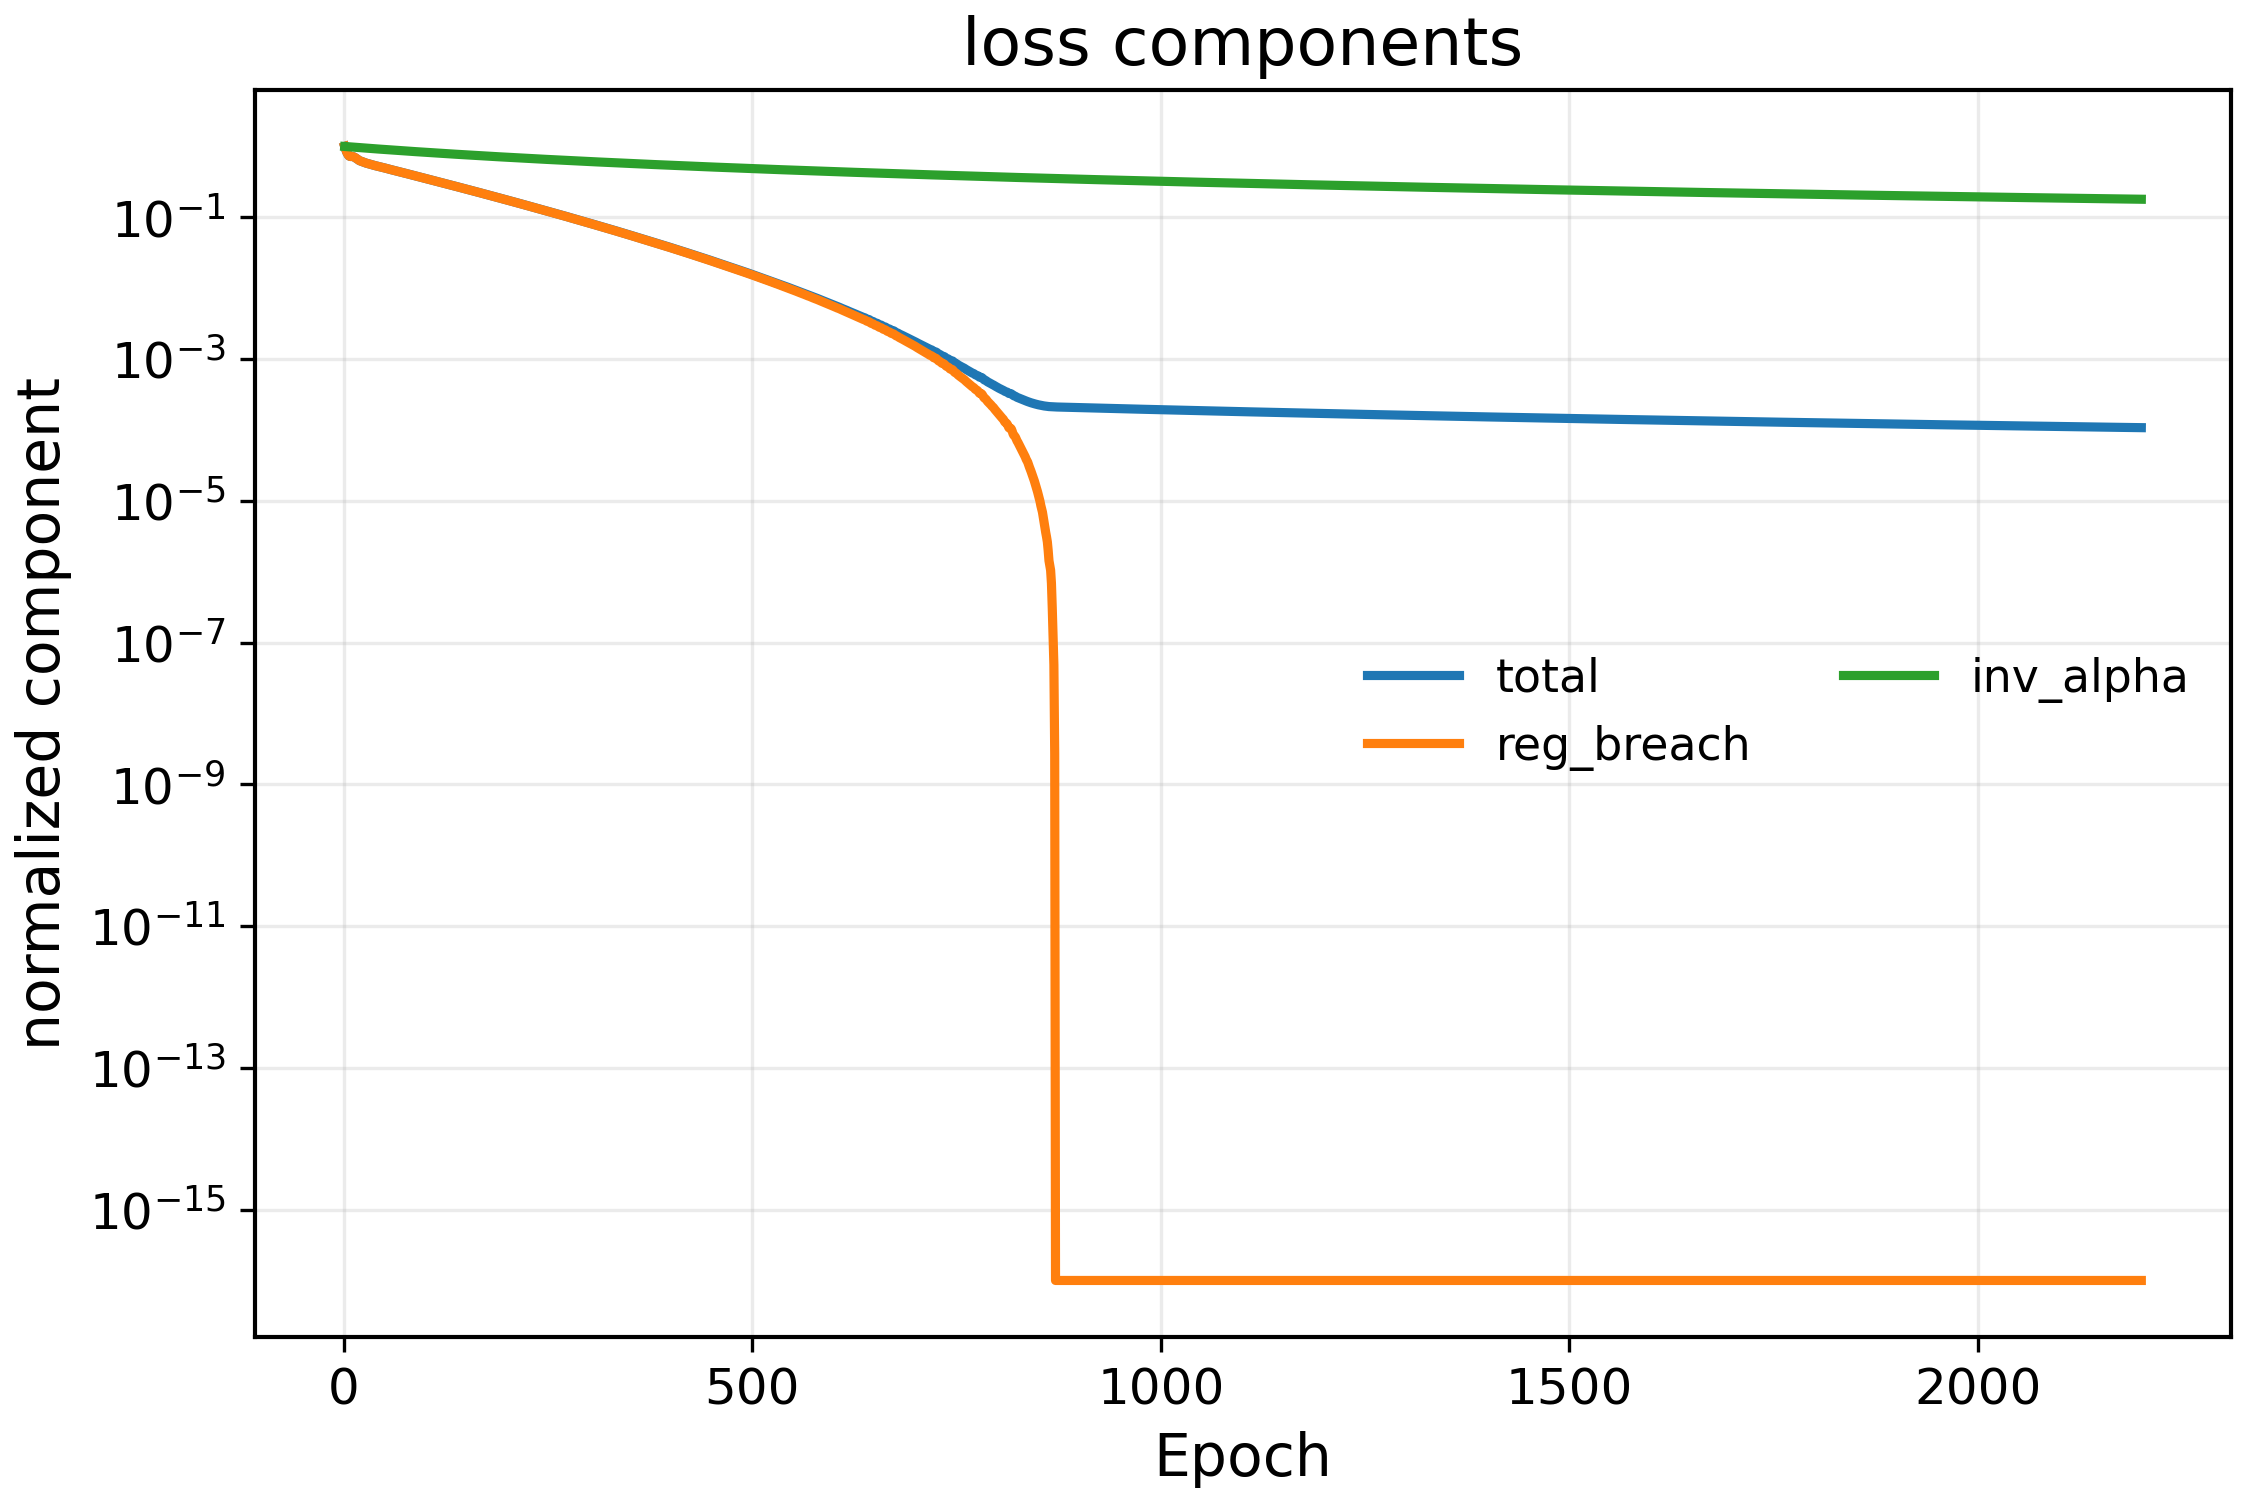
\includegraphics[width=\linewidth]{figures/domain_2_v_0p1_t_30p0_loss_components.png}
    \caption{Loss components across epochs.}
    \label{fig:d2-loss-components}
  \end{subfigure}\hfill
  \begin{subfigure}[t]{0.47\textwidth}
    \centering
    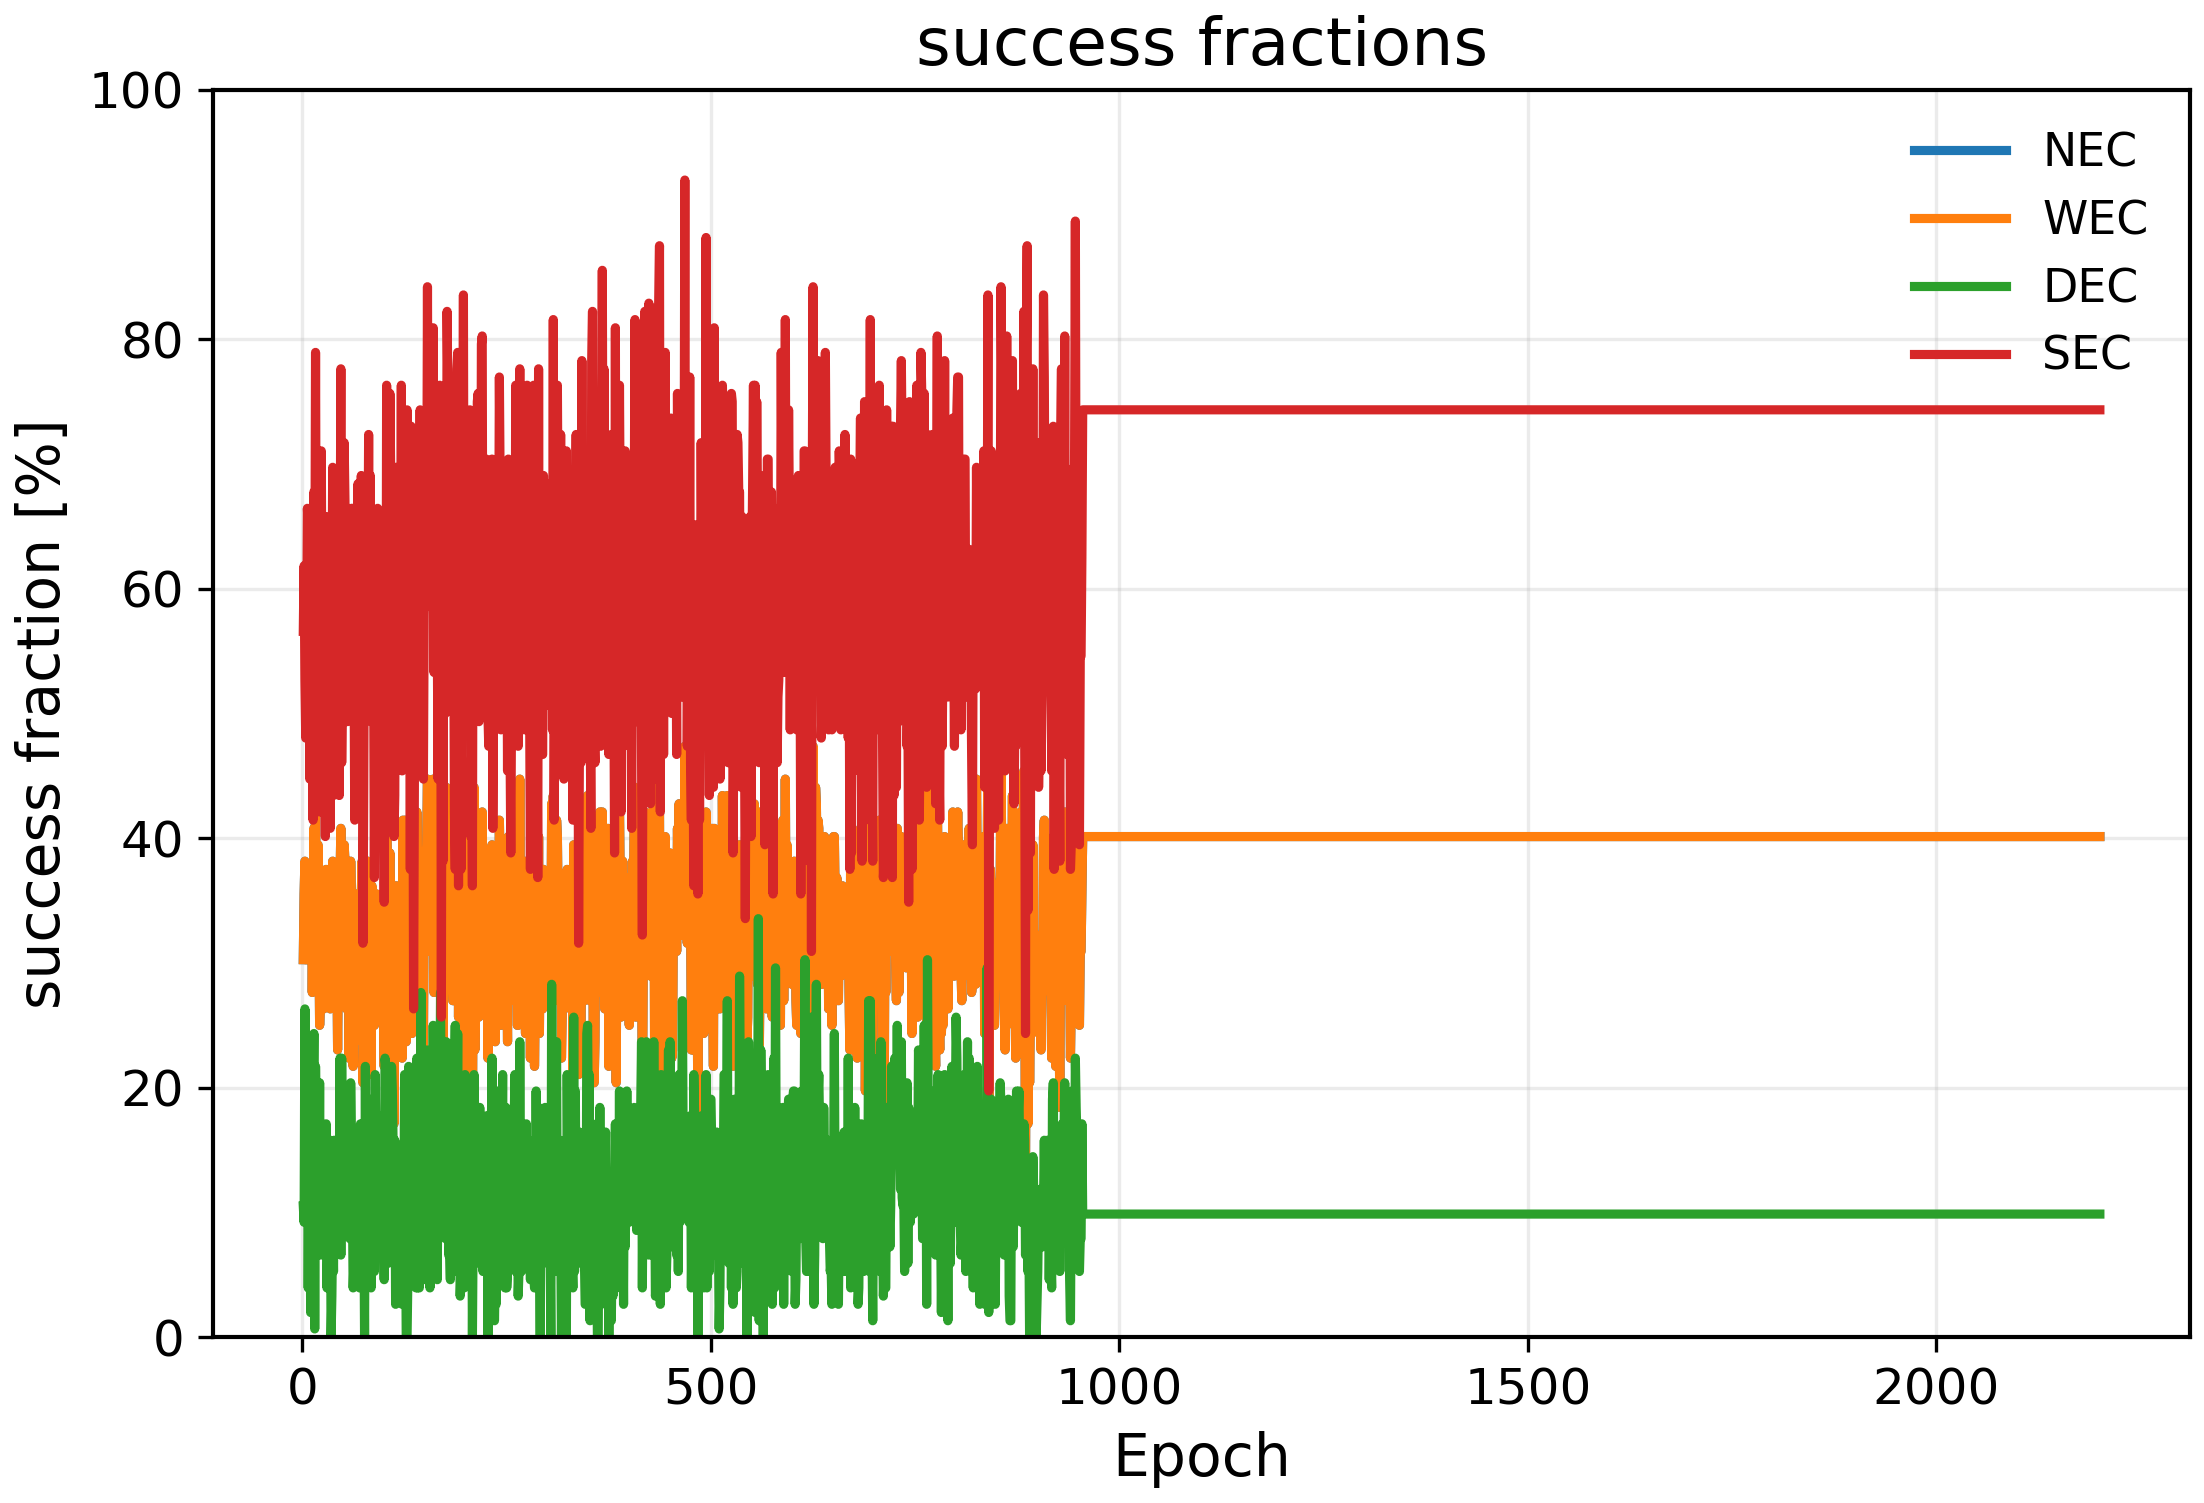
\includegraphics[width=\linewidth]{figures/domain_2_v_0p1_t_30p0_success_fractions.png}
    \caption{Success fractions for NEC/WEC/DEC/SEC.}
    \label{fig:d2-success}
  \end{subfigure}

  \vspace{1ex}

  \begin{subfigure}[t]{0.62\textwidth}
    \centering
    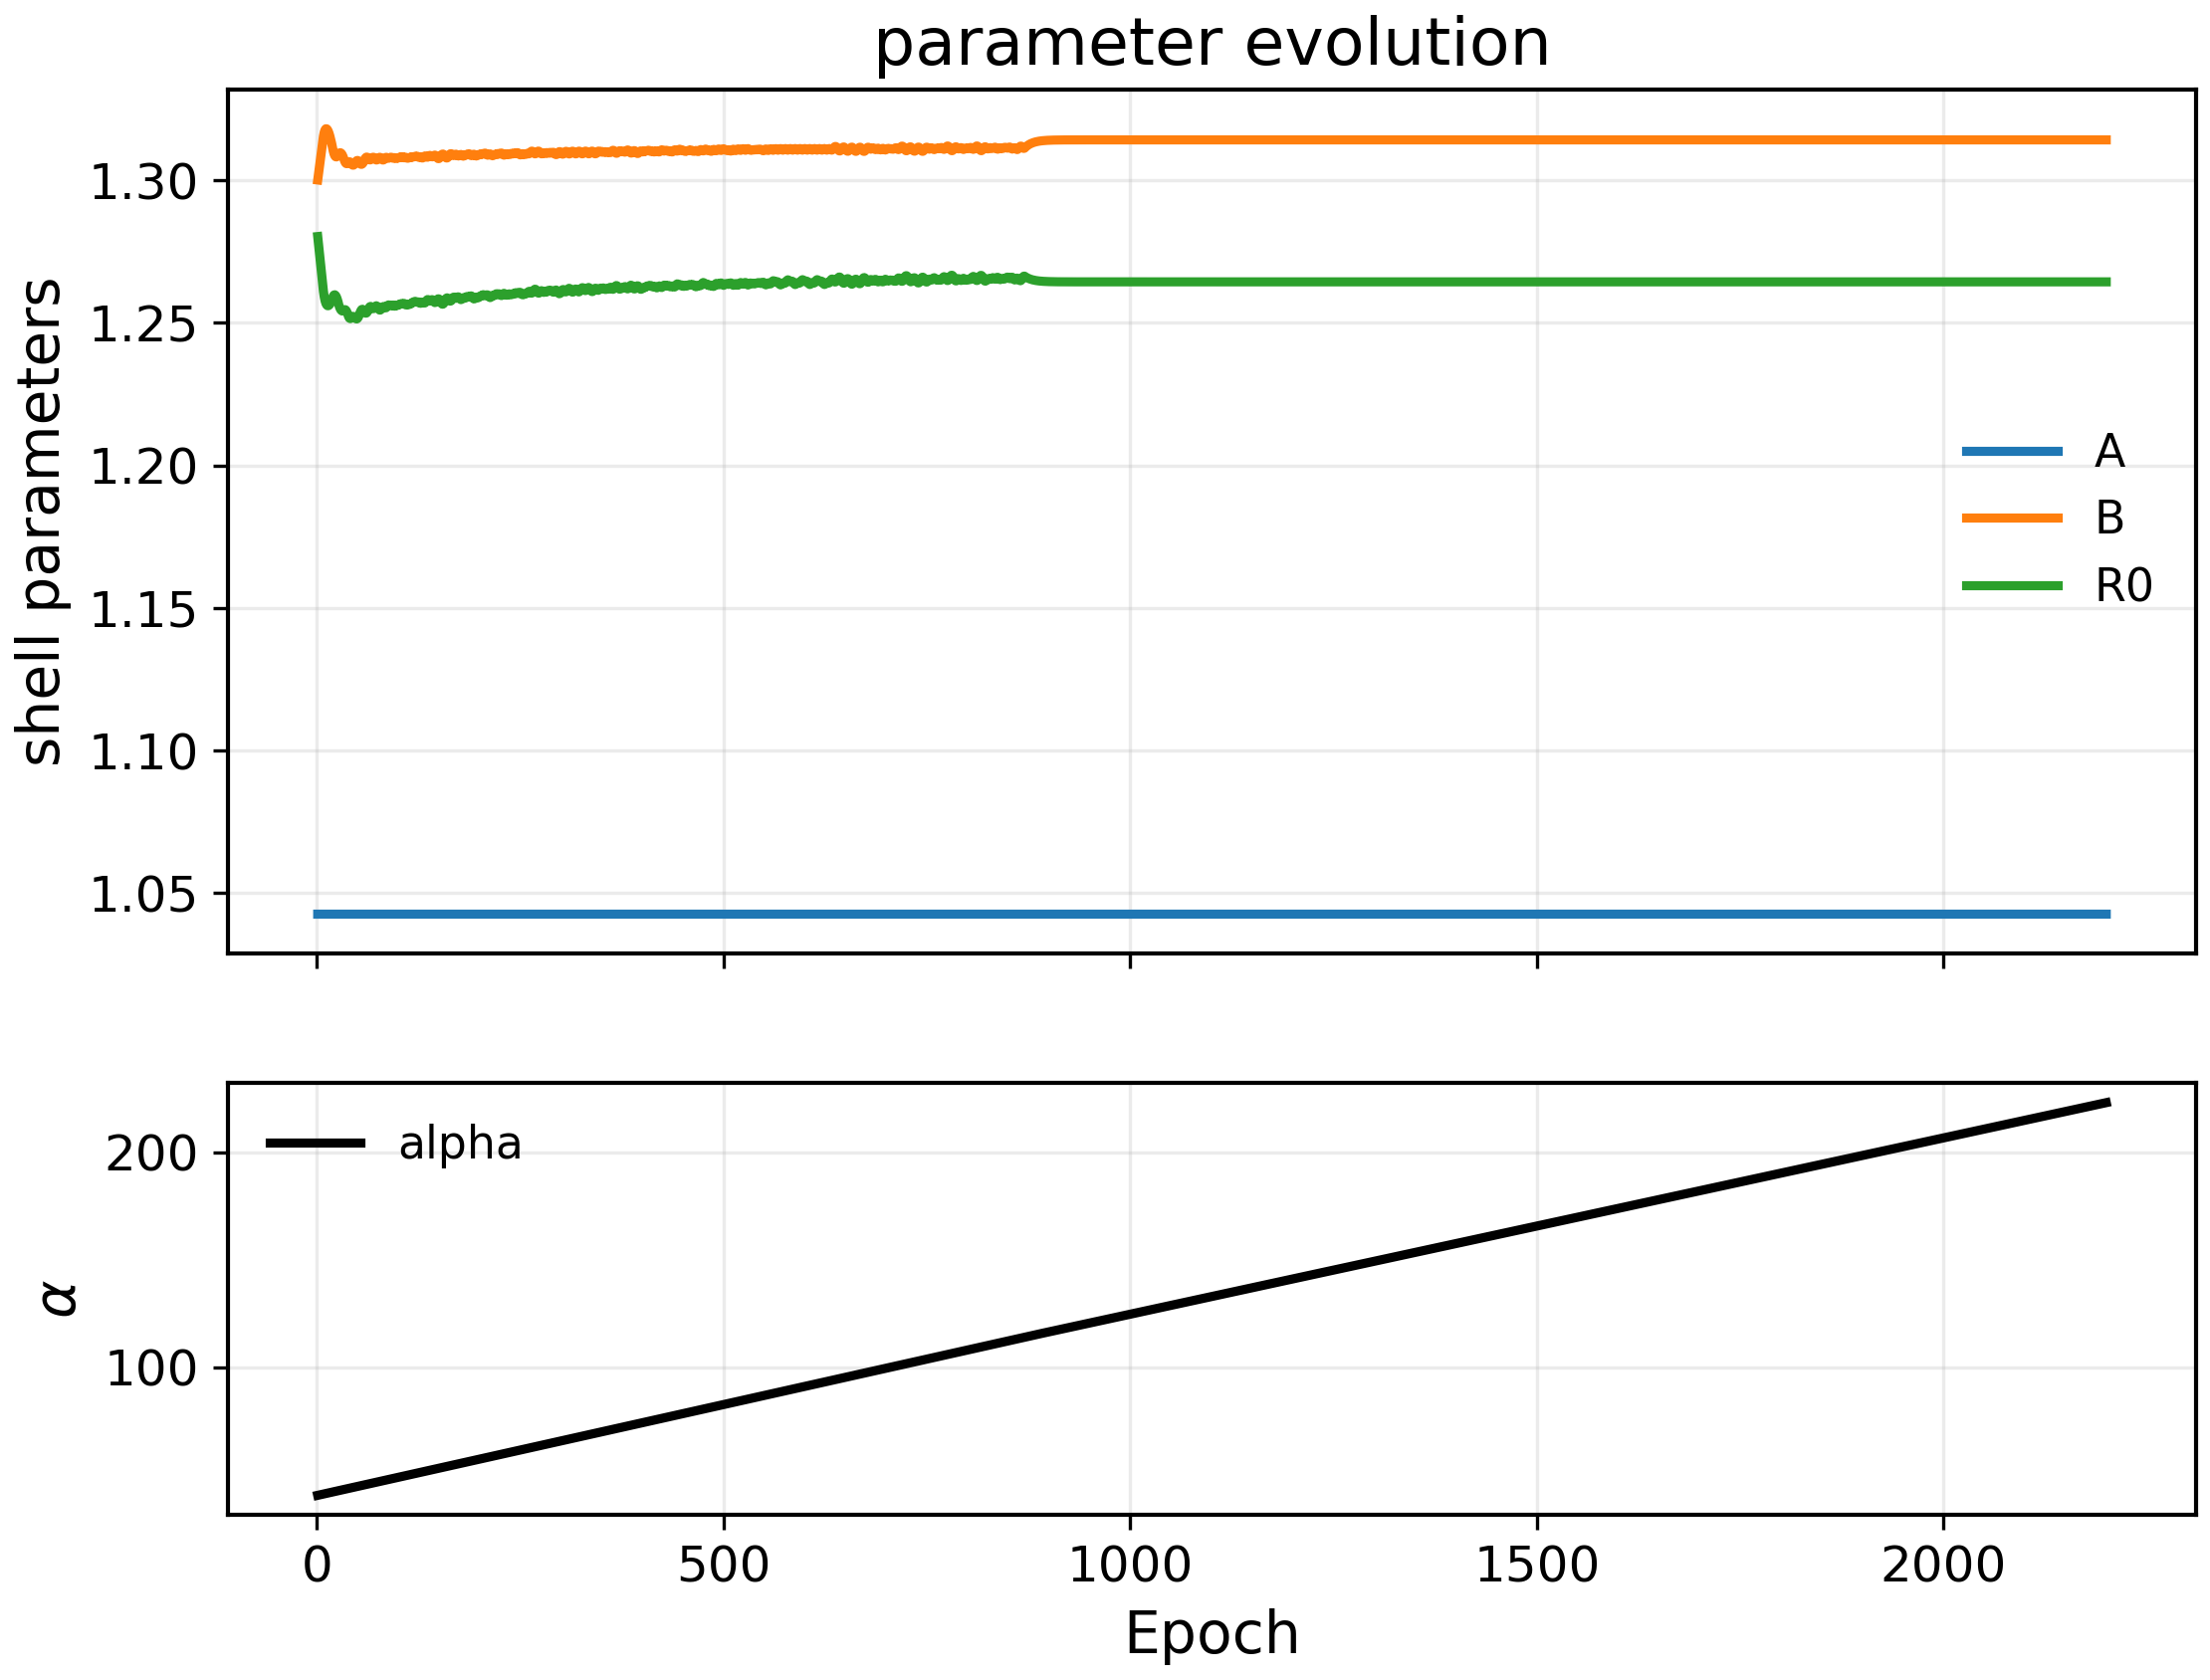
\includegraphics[width=\linewidth]{figures/domain_2_v_0p1_t_30p0_params.png}
    \caption{Seed parameters $A$, $B$, and $R_0$ across epochs.}
    \label{fig:d2-params-epoch}
  \end{subfigure}

  \caption{Optimization diagnostics for the double-shell configuration at $v=0.1$, $t=30$. Panel (a) shows the normalized loss terms \texttt{inv\_alpha}, \texttt{physics\_loss}, \texttt{reg\_breach}, and \texttt{total\_loss}. Panel (b) reports the fractions of grid points satisfying NEC/WEC/DEC/SEC; the double-shell case settles into a constrained regime in which SEC remains the easiest condition to satisfy, NEC/WEC stay above DEC, and DEC remains the tightest global constraint. Panel (c) shows that after a modest early adjustment the main run remains in a narrow band of $A$, $B$, and $R_0$, indicating a stable but more strongly constrained configuration within the adopted loss and diagnostic choices.}

  \label{fig:d2-opt}
\end{figure}


\FloatBarrier

\section*{Code and Data Availability}
The code and processed outputs used in this study are openly archived in the Zenodo software release~\citep{Bolivar_Abellan_Vasilev_2026_warp_optimization}. Following standard software-citation practice, we cite the exact version used for the manuscript. The cited release is version~v1.0.0, DOI: \url{https://doi.org/10.5281/zenodo.19243159}, and is distributed under the MIT License. The archive contains the optimization, diagnostics, plotting, and verification workflow, together with the regenerated single-shell and double-shell golden bundles and direct evaluations of the manuscript target parameters under the same diagnostics. These materials are sufficient to reproduce the reported bundle summaries and field-map figures.

%=================== APPENDICES ===================
\appendix

\section{Self-contained derivation of the translated Einstein tensor}
\label{app:translated-Gab}

This appendix provides the step-by-step derivation of the key structural result used in Sec.~\ref{sec:warp}: that a spatially uniform, time-independent centroid translation leaves $G_{00}$ and $G_{0i}$ unchanged while modifying only the spatial components $G_{ij}$. Rather than relying solely on the citations to Refs.~\cite{Santiago:2021aup,Schuster:2023ADMmass}, we present here a self-contained proof within the ADM formalism for the specific metric class considered in this paper.

\subsection{Setup and notation}
We work with the translated zero-vorticity line element in comoving Cartesian coordinates (Eq.~\eqref{eq:comoving-line-element}),
\begin{equation}
\label{eq:app-metric}
ds^2 = -dt^2 + \delta_{ij}\bigl(dx^i - \beta^i\,dt\bigr)\bigl(dx^j - \beta^j\,dt\bigr),
\end{equation}
where the total shift decomposes as
\begin{equation}
\label{eq:app-shift}
\beta^i(t,\vec x) = \beta(r)\,\hat r^i + v_*^i,
\end{equation}
with $r = \|\vec x\|$, $\hat r^i = x^i/r$, and $v_*^i = \text{const}$. The lapse is $N = 1$ (unit lapse) and the spatial metric is flat, $\gamma_{ij} = \delta_{ij}$.

\subsection{Extrinsic curvature}
For unit lapse and flat spatial slices, the extrinsic curvature of the constant-$t$ hypersurfaces is
\begin{equation}
K_{ij} = \frac{1}{2}\bigl(\partial_i \beta_j + \partial_j \beta_i\bigr).
\end{equation}
Since $v_*^i$ is spatially constant, $\partial_i v_*^j = 0$, and therefore
\begin{equation}
\label{eq:app-Kij-invariance}
K_{ij} = \frac{1}{2}\bigl(\partial_i [\beta(r)\hat r_j] + \partial_j [\beta(r)\hat r_i]\bigr),
\end{equation}
which depends only on $\beta(r)$ and is \emph{completely independent} of $v_*^i$. Explicitly, carrying out the spatial differentiation of $\beta(r)\hat r_i = \beta(r)\,x_i/r$,
\begin{equation}
\partial_j\bigl[\beta(r)\,\hat r_i\bigr] = \beta'(r)\,\hat r_j\,\hat r_i + \frac{\beta(r)}{r}\bigl(\delta_{ij} - \hat r_i \hat r_j\bigr),
\end{equation}
so
\begin{equation}
\label{eq:app-Kij-explicit}
K_{ij} = \frac{\beta(r)}{r}\,\delta_{ij} + \left[\beta'(r) - \frac{\beta(r)}{r}\right]\hat r_i\,\hat r_j.
\end{equation}
Its trace is
\begin{equation}
\label{eq:app-K-trace}
K \equiv K^i{}_i = \frac{2\beta(r)}{r} + \beta'(r).
\end{equation}
Both $K_{ij}$ and $K$ are functions of $r$ alone, with no dependence on the boost velocity.

\subsection{ADM constraint equations}

In the ADM decomposition with $N=1$ and $\gamma_{ij}=\delta_{ij}$, the Einstein tensor components in the orthonormal frame split into:

\paragraph{Hamiltonian constraint (energy density).}
\begin{equation}
\label{eq:app-G00}
G_{00} = \frac{1}{2}\bigl(K^2 - K_{ij}K^{ij}\bigr),
\end{equation}
where we have used ${}^{(3)}\!R = 0$ for flat spatial slices. Substituting Eqs.~\eqref{eq:app-Kij-explicit} and~\eqref{eq:app-K-trace},
\begin{equation}
K_{ij}K^{ij} = \frac{3\beta^2}{r^2} + \Bigl(\beta' - \frac{\beta}{r}\Bigr)^2 + \frac{2\beta}{r}\Bigl(\beta' - \frac{\beta}{r}\Bigr) = \frac{\beta^2}{r^2} + \frac{2\beta\beta'}{r} + (\beta')^2 - \frac{2\beta^2}{r^2} + \frac{3\beta^2}{r^2},
\end{equation}
which after simplification yields
\begin{equation}
G_{00} = \frac{\beta}{r^2}\bigl(2r\beta' + \beta\bigr),
\end{equation}
reproducing Eq.~(7) of the main text. Since $K_{ij}$ is independent of $v_*^i$, so is $G_{00}$.

\paragraph{Momentum constraint (energy flux).}
\begin{equation}
\label{eq:app-G0i}
G_{0i} = D_j\bigl(K^j{}_i - K\,\delta^j{}_i\bigr) = \partial_j K^j{}_i - \partial_i K,
\end{equation}
where $D_j = \partial_j$ for flat $\gamma_{ij}$. Since $K^j{}_i$ and $K$ depend only on $r$ and are independent of $v_*^i$, so is $G_{0i}$. We now show that $G_{0i}$ vanishes identically by explicit computation in Appendix~\ref{app:qi-vanishes}.

\paragraph{Spatial components (stresses).}
For unit lapse, the spatial components of the Einstein tensor involve $K_{ij}$, the time derivative $\dot K_{ij} = \partial_t K_{ij}$, and curvature terms. For a time-independent shift in comoving coordinates the full expression is
\begin{equation}
G_{ij} = (G_0)_{ij} + v_*^k\,\partial_k\bigl[K_{ij} - K\,\delta_{ij}\bigr],
\end{equation}
where $(G_0)_{ij}$ denotes the spatial Einstein-tensor components of the static seed. This additional term arises from the Lie transport of $K_{ij}$ along the boost direction and is the only place where $v_*^i$ enters the Einstein tensor.

\subsection{Summary}
Collecting these results, the Einstein tensor for the translated metric takes the form
\begin{align}
G_{00} &= (G_0)_{00}, \\
G_{0i} &= (G_0)_{0i} = 0, \\
G_{ij} &= (G_0)_{ij} + v_*^k\,\partial_k\bigl[K_{ij} - K\,\delta_{ij}\bigr],
\end{align}
confirming Eq.~(28) of the main text. The stress-energy tensor inherits the same structure via $T_{ab} = G_{ab}/(8\pi)$.


\section{Hawking--Ellis Type~I classification and all-observer energy conditions}
\label{app:type1}
\label{app:qi-vanishes}

A central concern raised in the evaluation of the present construction is whether the principal-stress energy-condition diagnostics, which are formulated in the orthonormal comoving frame, extend to \emph{all} timelike and null observers. This appendix proves that they do, by establishing the Hawking--Ellis Type~I classification~\cite{HawkingEllis1973} of the stress-energy tensor for the metric class considered in this paper.

\subsection{Vanishing of the momentum density \texorpdfstring{$q_i$}{qi}}

In the orthonormal comoving frame defined in Sec.~\ref{sec:warp}, the stress-energy tensor has the general form
\begin{equation}
T^a{}_b = \begin{pmatrix} -\rho & q_j \\ -q_i & P^i{}_j \end{pmatrix},
\end{equation}
where $\rho$ is the energy density, $q_i$ the energy flux (momentum density), and $P^i{}_j$ the spatial pressure tensor. We now prove that $q_i \equiv 0$ for the translated zero-vorticity ansatz with uniform centroid velocity.

From the ADM momentum constraint (Eq.~\eqref{eq:app-G0i}),
\begin{equation}
8\pi\,q_i = G_{0i} = \partial_j K^j{}_i - \partial_i K.
\end{equation}
Using the decomposition $K^j{}_i = A(r)\,\delta^j{}_i + B(r)\,\hat r^j\,\hat r_i$ with
\begin{equation}
A(r) \equiv \frac{\beta(r)}{r}, \qquad B(r) \equiv \beta'(r) - \frac{\beta(r)}{r},
\end{equation}
we compute each term. For the divergence of $K^j{}_i$:
\begin{align}
\partial_j K^j{}_i &= \partial_i A + \partial_j\bigl(B\,\hat r^j\,\hat r_i\bigr) \notag\\
&= A'\,\hat r_i + B'\,\hat r_i + B\,\hat r_i\,\underbrace{\partial_j \hat r^j}_{= 2/r} + B\,\hat r^j\,\underbrace{\partial_j \hat r_i}_{= (\delta_{ij} - \hat r_i \hat r_j)/r}\,\hat r^j \notag\\
&= A'\,\hat r_i + B'\,\hat r_i + \frac{2B}{r}\,\hat r_i,
\end{align}
where in the last step we used $\hat r^j \partial_j \hat r_i = 0$ (the radial derivative of the unit radial vector vanishes). For the gradient of the trace:
\begin{equation}
\partial_i K = K'\,\hat r_i = \left(\frac{2B}{r} + \beta''\right)\hat r_i,
\end{equation}
where we used $K = 3A + B = 2\beta/r + \beta'$ and computed
\begin{equation}
K' = \frac{d}{dr}\!\left(\frac{2\beta}{r} + \beta'\right) = \frac{2(\beta'r - \beta)}{r^2} + \beta'' = \frac{2B}{r} + \beta''.
\end{equation}
Substituting the radial derivatives $A' = B/r$ and $B' = \beta'' - B/r$ and combining:
\begin{align}
8\pi\,q_i &= \left(A' + B' + \frac{2B}{r}\right)\hat r_i - \left(\frac{2B}{r} + \beta''\right)\hat r_i \notag\\
&= \left(\frac{B}{r} + \beta'' - \frac{B}{r} + \frac{2B}{r} - \frac{2B}{r} - \beta''\right)\hat r_i \notag\\
&= 0.
\end{align}
This cancellation is \emph{exact and algebraic}: it holds for any smooth $\beta(r)$, at every spatial point, and independently of the boost velocity $v_*^i$. The energy flux vanishes identically in the orthonormal comoving frame.

\subsection{Block-diagonal structure implies Type~I}

With $q_i = 0$ established, the stress-energy tensor in the orthonormal frame is block-diagonal:
\begin{equation}
\label{eq:Tab-block}
T^a{}_b = \mathrm{diag}(-\rho,\; P^i{}_j).
\end{equation}
The spatial block $P^i{}_j$ is a real symmetric $3\times 3$ matrix (with respect to the flat spatial metric $\delta_{ij}$), so it is always diagonalizable with real eigenvalues $\lambda_1 \le \lambda_2 \le \lambda_3$. In the principal-pressure frame,
\begin{equation}
T^a{}_b = \mathrm{diag}(-\rho,\;\lambda_1,\;\lambda_2,\;\lambda_3).
\end{equation}
This is the canonical form of a Hawking--Ellis Type~I stress-energy tensor~\cite{HawkingEllis1973,Maeda:2022vld}: one timelike eigenvector (with eigenvalue $-\rho$) and three spacelike eigenvectors (with eigenvalues $\lambda_i$). The classification is valid at every point where the eigenvalues are well-defined, which for our smooth $\beta(r)$ is the entire computational domain excluding $r=0$ (where the coordinate system degenerates).

\subsection{Reduction of energy conditions to algebraic inequalities}

For a Type~I stress-energy tensor, the standard pointwise energy conditions are \emph{necessary and sufficient} conditions on the eigenvalues $\{-\rho, \lambda_1, \lambda_2, \lambda_3\}$~\cite{HawkingEllis1973,MartinMoruno:2017exc}. Specifically:

\begin{proposition}[All-observer energy conditions for Type~I]
\label{prop:type1-ec}
Let $T^a{}_b$ be Hawking--Ellis Type~I with timelike eigenvalue $-\rho$ and spatial eigenvalues $\lambda_1,\lambda_2,\lambda_3$. Then the pointwise energy conditions for \emph{all} timelike or null observers are equivalent to:
\begin{align}
\NEC &\iff \rho + \lambda_i \ge 0 \quad \text{for all } i \in \{1,2,3\}, \label{eq:nec-type1}\\
\WEC &\iff \rho \ge 0 \;\;\text{and}\;\; \rho + \lambda_i \ge 0 \quad \text{for all } i, \label{eq:wec-type1}\\
\DEC &\iff \rho \ge 0 \;\;\text{and}\;\; \rho \ge |\lambda_i| \quad \text{for all } i, \label{eq:dec-type1}\\
\SEC &\iff \rho + \lambda_i \ge 0 \;\;\text{for all } i \;\;\text{and}\;\; \rho + \textstyle\sum_i \lambda_i \ge 0. \label{eq:sec-type1}
\end{align}
\end{proposition}

\noindent The proof is standard (see e.g.\ \cite{HawkingEllis1973}, Ch.~4.3; \cite{MartinMoruno:2017exc}, Sec.~II). We sketch it for completeness. For the \WEC, one must show $T_{ab}u^a u^b \ge 0$ for all future-directed timelike $u^a$. Decomposing $u^a = \gamma(e_0^a + v^i e_i^a)$ with $\gamma = (1-\delta_{ij}v^iv^j)^{-1/2}$ and $|v|<1$, one finds
\begin{equation}
T_{ab}\,u^a u^b = \gamma^2\!\left(\rho + \sum_i \lambda_i (v^i)^2\right),
\end{equation}
where we used the principal frame so that $P_{ij} = \mathrm{diag}(\lambda_1,\lambda_2,\lambda_3)$. For this to be non-negative for all $|v|<1$, it is necessary and sufficient that $\rho \ge 0$ (taking $v\to 0$) and $\rho + \lambda_i \ge 0$ (taking $v^i \to 1$ along each axis). The null case (\NEC) follows by the limiting procedure $|v|\to 1$. The \DEC\ and \SEC\ conditions follow by analogous algebraic arguments.

\subsection{Implications for the present construction}

The combination of the results in this appendix establishes the following:

\begin{enumerate}
\item The energy flux $q_i$ vanishes identically for the translated zero-vorticity ansatz with uniform $v_*^i$, so $T^a{}_b$ is block-diagonal in the orthonormal comoving frame.
\item The spatial pressure tensor $P_{ij}$ is real and symmetric, so $T^a{}_b$ is Hawking--Ellis Type~I at every regular grid point.
\item By Proposition~\ref{prop:type1-ec}, the principal-stress margins
\begin{equation}
m_\NEC = \rho + \lambda_{\min},\quad m_\WEC = \rho + \min(\lambda_{\min},0),\quad m_\DEC = \rho - |\lambda|_{\max},\quad m_\SEC = \rho + \textstyle\sum_i\lambda_i
\end{equation}
are \emph{necessary and sufficient} for the corresponding energy conditions to hold for \emph{all} timelike and null observers, not merely for the comoving observer.
\end{enumerate}

This upgrades the diagnostic status of the numerical pipeline: the margins reported in Sec.~\ref{sec:numerics} and shown in Figs.~\ref{fig:d1-xy-energy-A}--\ref{fig:d2-xz-energy-B} are all-observer energy-condition tests within the Type~I regime, not just preferred-frame checks. The Type~I classification is verified numerically at every grid point as part of the diagnostic workflow (see Code and Data Availability).


\bibliographystyle{unsrtnat}
\bibliography{warpdrive1,warpdrive_zenodo}

\end{document}







